\documentclass[11pt,]{article}
\usepackage{lmodern}
\usepackage{amssymb,amsmath}
\usepackage{ifxetex,ifluatex}
\usepackage{fixltx2e} % provides \textsubscript
\ifnum 0\ifxetex 1\fi\ifluatex 1\fi=0 % if pdftex
  \usepackage[T1]{fontenc}
  \usepackage[utf8]{inputenc}
\else % if luatex or xelatex
  \ifxetex
    \usepackage{mathspec}
  \else
    \usepackage{fontspec}
  \fi
  \defaultfontfeatures{Ligatures=TeX,Scale=MatchLowercase}
\fi
% use upquote if available, for straight quotes in verbatim environments
\IfFileExists{upquote.sty}{\usepackage{upquote}}{}
% use microtype if available
\IfFileExists{microtype.sty}{%
\usepackage{microtype}
\UseMicrotypeSet[protrusion]{basicmath} % disable protrusion for tt fonts
}{}
\usepackage[margin=1.0in]{geometry}
\usepackage{hyperref}
\hypersetup{unicode=true,
            pdftitle={Who are ASM Journals? A Gender-based Analysis},
            pdfborder={0 0 0},
            breaklinks=true}
\urlstyle{same}  % don't use monospace font for urls
\usepackage{graphicx,grffile}
\makeatletter
\def\maxwidth{\ifdim\Gin@nat@width>\linewidth\linewidth\else\Gin@nat@width\fi}
\def\maxheight{\ifdim\Gin@nat@height>\textheight\textheight\else\Gin@nat@height\fi}
\makeatother
% Scale images if necessary, so that they will not overflow the page
% margins by default, and it is still possible to overwrite the defaults
% using explicit options in \includegraphics[width, height, ...]{}
\setkeys{Gin}{width=\maxwidth,height=\maxheight,keepaspectratio}
\IfFileExists{parskip.sty}{%
\usepackage{parskip}
}{% else
\setlength{\parindent}{0pt}
\setlength{\parskip}{6pt plus 2pt minus 1pt}
}
\setlength{\emergencystretch}{3em}  % prevent overfull lines
\providecommand{\tightlist}{%
  \setlength{\itemsep}{0pt}\setlength{\parskip}{0pt}}
\setcounter{secnumdepth}{0}
% Redefines (sub)paragraphs to behave more like sections
\ifx\paragraph\undefined\else
\let\oldparagraph\paragraph
\renewcommand{\paragraph}[1]{\oldparagraph{#1}\mbox{}}
\fi
\ifx\subparagraph\undefined\else
\let\oldsubparagraph\subparagraph
\renewcommand{\subparagraph}[1]{\oldsubparagraph{#1}\mbox{}}
\fi

%%% Use protect on footnotes to avoid problems with footnotes in titles
\let\rmarkdownfootnote\footnote%
\def\footnote{\protect\rmarkdownfootnote}

%%% Change title format to be more compact
\usepackage{titling}

% Create subtitle command for use in maketitle
\newcommand{\subtitle}[1]{
  \posttitle{
    \begin{center}\large#1\end{center}
    }
}

\setlength{\droptitle}{-2em}

  \title{\textbf{Who are ASM Journals? A Gender-based Analysis}}
    \pretitle{\vspace{\droptitle}\centering\huge}
  \posttitle{\par}
    \author{}
    \preauthor{}\postauthor{}
    \date{}
    \predate{}\postdate{}
  
\usepackage{booktabs}
\usepackage{longtable}
\usepackage{array}
\usepackage{multirow}
\usepackage[table]{xcolor}
\usepackage{wrapfig}
\usepackage{float}
\usepackage{colortbl}
\usepackage{pdflscape}
\usepackage{tabu}
\usepackage{threeparttable}
\usepackage{threeparttablex}
\usepackage[normalem]{ulem}
\usepackage{makecell}
\usepackage{caption}

\usepackage{helvet} % Helvetica font
\renewcommand*\familydefault{\sfdefault} % Use the sans serif version of the font
\usepackage[T1]{fontenc}

\usepackage[none]{hyphenat}

\usepackage{setspace}
\doublespacing
\setlength{\parskip}{1em}

\usepackage{lineno}

\usepackage{pdfpages}
\floatplacement{figure}{H} % Keep the figure up top of the page
\usepackage{booktabs}
\usepackage{longtable}
\usepackage{array}
\usepackage{multirow}
\usepackage{wrapfig}
\usepackage{float}
\usepackage{colortbl}
\usepackage{pdflscape}
\usepackage{tabu}
\usepackage{threeparttable}
\usepackage{threeparttablex}
\usepackage[normalem]{ulem}
\usepackage{makecell}
\usepackage{xcolor}

\begin{document}
\maketitle

\vspace{35mm}

Running title: A gender-based analysis of ASM journals

\vspace{35mm}

Ada K. Hagan\({^1}\), Begüm D. Topçuoğlu\({^1}\), Hazel Barton\({^2}\),
Patrick D. Schloss\textsuperscript{1\(\dagger\)}

\vspace{40mm}

\(\dagger\) To whom correspondence should be addressed:
\href{mailto:pschloss@umich.edu}{\nolinkurl{pschloss@umich.edu}}

1. Department of Microbiology and Immunology, University of Michigan,
Ann Arbor, MI 48109

2. Department of Biology, University of Akron, Akron, OH

\newpage

\linenumbers

\subsection{Abstract}\label{abstract}

Evidence has accumulated over the decades that academic research has a
representation problem. While at least 50\% of biology Ph.D.~graduates
are women, the number of women in postdoctoral positions and
tenure-track positions are below 40\% and 30\%, respectively. Recently,
scientific societies and publishers have begun examining internal
submissions data to evaluate representation of, or bias against, women
in their peer review processes; however, representation and attitudes
differ by scientific field and no studies to-date seem to have
investigated academic publishing in the field of microbiology. Using
manuscripts submitted between January 2012 and August 2018 to 13
journals published by the American Society for Microbiology (ASM), we
describe the representation of women at ASM journals and the outcomes of
their manuscripts. We find that senior women authors at ASM journals are
underrepresented compared to global and society estimates of
microbiology researchers. Additionally, manuscripts submitted by
corresponding authors that were women, received more negative outcomes
(e.g., editorial rejections, reviewer recommendations, and decisions
after review), than those submitted by men. These negative outcomes were
somewhat mediated by whether or not the corresponding author was based
in the US or not, and by the institution for US-based authors.
Nonetheless, the pattern for women corresponding authors to receive more
negative outcomes for their submitted manuscripts indicates a pattern of
gender-influenced editorial decisions. We conclude with suggestions to
improve the representation of, and decrease bias against, women at ASM
journals.

\subsection{Importance}\label{importance}

Women are underrepresented as senior scientists at ASM journals. This is
due to a combination of both low submissions from senior women authors
and increased rejection rates for women compared to men.

\subsection{Introduction}\label{introduction}

Evidence has accumulated over the decades that academic research has a
representation problem. While at least 50\% of biology Ph.D.~graduates
are women, the number of women in postdoctoral positions and
tenure-track positions are less than 40 and 30\%, respectively (1).
Studies examining other metrics such as race and ethnicity found that in
2011, less than 27\% of all science and engineering doctorates were
awarded to underrepresented minorities, and less than 25\% of associate
professors identified as non-white (2, 3). Predictably, the disparities
increase with academic rank (4). There have been many proposed reasons
for these disparities, particularly with regards to women, which include
biases in training and hiring, the impact of children on career
trajectories, a lack of support for primary caregivers, a lack of
recognition, lower perceived competency, and less productivity as
measured by research publications (1, 5--9). These issues do not act
independent of each other, instead they are cumulative over time for
both individuals and the community, much as advantages accumulate (10,
11). Accordingly, addressing these issues necessitates multi-level
approaches from all institutions and members of the scientific
community.

Scientific societies play an integral role in the formation and
maintenance of scientific communities. They host conferences that
provide a forum for knowledge exchange, networking, and opportunities
for increased visibility as a researcher. Scientific societies also
frequently publish the most reputable journals in their field,
facilitating the peer review process to vet new research submissions.
Recently, scientific societies and publishers have begun examining
internal submissions data to evaluate representation of, and bias
against, women in their peer review processes. The American Geological
Union found that while the acceptance rate of women-authored
publications was greater than publications authored by men, women
submitted fewer manuscripts than men and were used as reviewers only
20\% of the time (12), a factor influenced by the gender of the editor
(13). Several other studies have concluded that there is no significant
bias against papers authored by women (13--17). Two recent studies---one
of the peer review process at eLife, a broad scope biology journal, and
the other of outcomes at six ecology and evolution journals---found that
women-authored papers are less likely to have positive peer reviews and
outcomes (18, 19).

The representation of women scientists and gender attitudes differ by
scientific field, and no studies to-date seem to have investigated
academic publishing in the field of microbiology. The American Society
for Microbiology (ASM) is one of the largest life science societies,
with an average membership of 41,000 since 1990. In its mission
statement, the ASM notes that it is ``an inclusive organization,
engaging with and responding to the needs of its diverse
constituencies'' and pledges to ``address all members' needs through
development and assessment of programs and services.'' One of these
services is the publication of microbiology research through a suite of
research and review journals. Between January 2012 and August 2018, ASM
published 15 different journals: \emph{Antimicrobial Agents and
Chemotherapy} (AAC), \emph{Applied and Environmental Microbiology}
(AEM), \emph{Clinical and Vaccine Immunology} (CVI), \emph{Clinical
Microbiology Reviews} (CMR), \emph{Eukaryotic Cell} (EC),
\emph{Infection and Immunity} (IAI), \emph{Journal of Bacteriology}
(JB), \emph{Journal of Clinical Microbiology} (JCM), \emph{Journal of
Virology} (JV), \emph{mBio}, \emph{Microbiology and Molecular Biology
Reviews} (MMBR), \emph{Genome Announcements} (GA, now \emph{Microbiology
Resource Annoucements}), \emph{Molecular and Cellular Biology} (MCB),
\emph{mSphere}, and \emph{mSystems}. The goal of this research study is
to describe the population of ASM journals through the representation of
authors, reviewers, and editors by gender and the associated peer review
outcomes of their manuscripts.

\subsection{Results}\label{results}

Over 100,000 manuscript records were obtained for the period between
January 2012 and August 2018 (Fig. 1). Many papers are immediately
rejected by editors instead of being sent to peer review, often due to
issues of scope or perceived quality. These were defined as editorial
rejections and identified as manuscripts rejected without record of
review. Alternately, editors could send papers out for review by two or
three experts in the field selected from a list of potential reviewers
in the manuscript records (whether they were author- or editor-suggested
is unknown). The reviewers make suggestions to the editor who decides
whether the manuscript in question should be accepted, rejected, or sent
back for revision. At ASM journals, manuscripts with suggested revisions
that are expected to take more than 30 days are rejected, but generally
encouraged to resubmit. If resubmitted, the authors are asked to note
the previous (related) manuscript and the re-submission is assigned a
new manuscript number. Multiple related manuscripts were tracked
together by generating a unique grouped manuscript number based on the
recorded related manuscript numbers. This grouped manuscript number
served dual purposes of tracking a single manuscript through multiple
rejections and avoiding duplicate counts of authors for a single
manuscript. After eliminating non-primary research articles and linking
records for resubmitted articles, there were 81,897 unique manuscripts
processed (Fig. 1).

We attempted to assign genders to both peer review gatekeepers (e.g.,
editor-in-chief, editors, reviewers) and authors on the original
research manuscripts evaluated during this time period. We recognize
that biological sex (male/female) is not always equivalent to the gender
that an individual presents as (man/woman), which is also distinct from
the gender(s) that an individual may self-identify as. For the purposes
of this manuscript, we choose to focus on the presenting gender
(man/woman/unknown) based on their first names (and appearance for
editors). Author genders were assigned using a social media-informed
predictive algorithm with stringent criteria and validation process (see
methods). This method of gender assignment resulted in a category of
individuals whose gender could not be reliably predicted. In the
interest of transparency, we include those individuals whose names don't
allow a high degree of confidence for gender assignment in the
``unknown'' category of our analysis, which is shown in many of the
plots depicting representation of the population, but are not included
in the comparison of manuscript outcomes.

\textbf{Men dominate as gatekeepers and senior authors.} We first
evaluated the representation of men and women who were gatekeepers at
ASM during the study period. Each journal is led by an editor-in-chief
(EIC) who manages journal scope and quality standards through a board of
editors with field expertise that handle the peer review process. In
total, there were 17 EICs, 17.65\% of which were women. Two journals, EC
and CVI were retired during the period under study. Four years before
retirement, the leadership of CVI transferred from a man EIC, to a woman
while JVI has had a woman as EIC since 2012. The total number of editors
at all ASM journals combined over the duration of our study (senior
editors and editors pooled) was 1016, 28.74\% of which were women.

Over 40\% of both men and women editors were from US-based R1
institutions, defined as doctoral universities with very high research
activity, with non-US institutions, and U.S. medical schools or research
institutions supplying the next largest proportions of editors (Fig.
2A). Since the start of our study, there has been a slow trend toward
equivalent gender representation among editors (Fig. 2B). The trends for
each journal studied vary considerably, though most have slow trends
toward parity (Fig. S1). CVI and \emph{mSphere} were the only ASM
journals to have accomplished equivalent representation of both genders,
with CVI having a greater proportion of women editors than men before it
was retired. EC is the only journal with an increasing parity gap.

Altogether, editors recruited a total of 30704 reviewers, 24.61\% of
which were women, to act as manuscript reviewers. The greatest
proportion of reviewers (over 50\% of both men and women) come from
non-US institutions, while R1 institutions supply the next largest
cohort of reviewers (Fig. 2C). Over the time period studied, the
proportions of each gender have held steady among reviewers at ASM
journals (Fig. 2D) and is representative of both the listed potential
reviewers at all journals combined, and the actual reviewer proportions
at most journals (Fig. S2).

\textbf{Editorial workloads were not proportionate} Across all journals,
men handle a slightly greater proportion of manuscripts (blue) than
women (orange), relative to their respective editorial representations
(Fig. 3A). This trend continues across most journals with varying
degrees of difference between workload and representation (Fig. S1). For
instance, at \emph{mSphere}, workload and proportions were identical;
however, CVI, \emph{mBio}, and JVI, each have points at which the
workload for women editors is much higher than their representation,
with corresponding decreases in the workload of men. In the years
preceding its retirement, the representation of women at CVI increased,
which acted to decrease the gap in editorial workload. However,
representations and relative workloads for men and women editors at JVI
have held steady over time, while the proportionate workload for women
at \emph{mBio} has increased.

Between 2012 and 2018, the median number of manuscripts reviewed by
individuals in each gender group is equivalent, at 2. Half of those in
men, women, or unknown gender groups reviewed between one and 5, 4, or 3
manuscripts each, respectively (Fig. 3B). Conversely, 43.35\% of men,
38.97\% of women, and 47.45\% of unknown gendered reviewers have
reviewed only one manuscript. Reviewers of all genders accepted fewer
requests to review from women editors (average of 47.91\%) than from men
(average of 53.4\%) and were less likely to respond to women editors
than men (no response rate averages of 25.04 and 19.91\%, respectively)
(Fig. 3C). Editors of both genders contacted reviewers from all three
gender groups at equivalent proportions, though women editors contact an
average of 76.29\% of potential reviewers, while men contact 73.92\% on
average (Fig. 3D).

\textbf{Women were underrepresented as authors} Globally, microbiology
researchers are 60\% men and 40\% women (20). At ASM in September 2018,
38.37\% of members who reported their gender were women. We wanted to
determine if these proportions were similar for authors at ASM journals
and to understand the distribution of each gender among submitted and
published manuscripts. We began by describing author institutions by
gender. Over 60\% of submitting authors were from non-US institutions,
followed by 20\% from R1 institutions (Fig. 4A). The proportions of men
and women authors at ASM have decreased over time at equivalent rates,
with a ratio of men to women authors of 4:3 since 2012 (or, 57\% men)
(Fig. 4B). The decrease in gendered authors corresponds with an increase
in the proportion of unknown gendered authors.

In the field of microbiology, order of authorship on manuscripts signal
the type and magnitude of contributions to the finished product with
first and last authorship being the most prestigious. First authors are
generally trainees (e.g., students or post-docs) or early career
research responsible for the bulk of the project, while last authors are
lead investigators, supplying conceptual guidance and resources to
complete the project. Middle authors are generally responsible for
technical analyses and methods. Any author can also be a corresponding
author, which we identified as the individual responsible for
communicating with publishing staff during peer review (as opposed to an
author to whom readers direct questions).

The proportion of papers submitted with men and women first authors have
remained constant with averages of 29.64 and 31.08 percent, respectively
(Fig. 4C, dashed). Their respective proportions of average published
manuscripts were nearly identical at 33.16\% for men and 33.85\% for
women. The proportion of submitted papers with men corresponding authors
has remained steady at an average of 42.45\% while the proportion with
women corresponding authors was at 23.56\% (Fig. 4D, dashed). Both men
and women corresponding authors have a greater proportion of manuscripts
published than were submitted, the difference where men were
corresponding authors is 7.4, and 0.79 for women corresponding authors.
This trend is similar for middle and last authors (Fig. S3).

Of 39168 manuscripts submitted by men corresponding authors, 23.52\% had
zero women authors (single author papers excluded). 7403 (36.45\%) of
papers submitted by women corresponding authors had at least 51\% of the
authors as women, exceeding those submitted by men corresponding authors
in both the number (3305) and percent (8.44) of submissions.
Additionally, the proportion of women authors decreases as the number of
authors increases (Fig. S4).

We hypothesized that we would be able to predict the gender of the
corresponding author from the manuscript metadata. We trained a logistic
regression model to predict the gender of the corresponding author using
whether or not the corresponding author's institution was in the U.S.,
the total number of authors, the proportion of authors that were women,
whether or not the article was published, the gender of senior editors
and editors, the number of revisions, and whether or not the manuscript
was editorially rejected as variables to train our model. If there is no
bias in collaborations, the model should not perform better than random
(0.5) at assigning gender to submissions, as measured by the area under
the receiver operating characteristic curve (AUROC). The AUROC value is
a predictive performance metric that ranges from 1.0, where the model
perfectly distinguishes between outcomes, to 0.0, where the model's
predictions completely wrong. The median AUROC value of our model to
predict corresponding author gender was 0.7. The variable with the
largest weight (i.e., the most predictive value), in our model was the
proportion of women authors. These results indicate that manuscript
submission data is capable of predicting the gender of the corresponding
author, but that prediction is primarily driven by what percentage of
authors are women.

To better visualize the 7.52\% decrease from the proportion of women who
were first authors, to those who were corresponding authors (Fig. 4CD),
we asked the proportions at which women have been retained through the
peer review system at ASM journals. During the period of time under
study, there were 76215 women who participated as junior authors
(first/middle) at ASM journals. Of those junior authors who were women,
8.25\% also participated as senior authors (last/corresponding), and
8.91\% were listed as potential reviewers. 5.39\% of the women junior
authors later participated as reviewers and 0.25\% were an editor. For
men, there were a total of 84482 junior authors, where 13.59\% were also
senior authors, 16.72\% considered as reviewers, and 11.11\% actually
reviewed. 0.66 of men junior authors were also editors at ASM journals.
Overall, women are half as likely to move to more prestigious (e.g.,
senior author, gatekeeper) roles in peer review than men are.

\textbf{Papers submitted by women have more negative outcomes than those
submitted by men.} To better understand the differences between
published and submitted proportions for men and women authors (Fig. 4CD,
Fig. S3), we compared the rejection rates of men and women at each
author stage (first, middle, corresponding, and last). Middle authors
were rejected at similar rates for men and women, a 0.01 percentage
point difference across all journals combined; however, manuscripts with
senior women authors were rejected more frequently than those authored
by men with -1.6 and -0.92 percentage point differences for
corresponding and last authors, respectively (Fig. 5A, vertical line).
There were several instances where the overall trend is repeated or even
amplified at the journal level (e.g., AAC, IAI, JB, \emph{mBio}, MCB).
The greatest effect was observed when comparing the outcome of
corresponding authors by gender, so we used this sub-population to
further examine the difference in manuscript acceptance and rejection
rates between men and women.

We next compared the rejection rates for men and women corresponding
authors after two bottlenecks, initial review by the editor and the
first peer review. Papers authored by women were editorially rejected as
much as 12 percentage points more often than those authored by men (Fig.
5B). The percentage point difference at all ASM journals combined is
-3.87 (vertical line), and two journals, MCB and \emph{mBio}, have more
extreme percentage point differences. Papers authored by men and women
were equally likely to be accepted after the first round of review (Fig.
5C, right panel). However, women-authored papers were rejected more
often (left panel) while men-authored papers were more often given
revision decisions (center panel). Three journals, JB, AAC, and MCB,
have percentage point differences more extreme than for all ASM journals
combined in both rejection and revision decisions, (-5.49 and 5.45
respectively; Fig. 5C vertical lines). Percentage point differences were
not correlated with journal prestige as measured by impact factors
(R\({^2}\) = -0.022).

In addition to manuscript decisions, other disparate outcomes may occur
during the peer review process (21). To determine whether accepted
women-authored manuscripts spent more time between being submitted and
being ready for publication, we compared the number of revisions, days
spent in the ASM peer review system, and the number of days from
submission to being ready for publication to those authored by men.
Papers authored by women take slightly longer (from submission to ready
for publication) than men at some journals (\emph{mSphere}, \emph{mBio},
\emph{mSystems}, CVI, JB, JCM, AEM) despite spending similar amounts of
time in the ASM journal peer review system, and having equivalent median
number of revisions prior to acceptance (Fig. S5).

To understand how gatekeeper (editor/reviewer) genders influence
decisions (e.g., Fig. 5C), we grouped editor decisions and reviewer
suggestions according to the gatekeeper gender. Both men and women
editors rejected proportionally more women-authored papers, with men
editors making revise decisions on papers authored by men more often
than those authored by women (Fig. 6A). Reviewers were more likely to
suggest rejection for women-authored manuscripts as compared to men,
though no difference in revise suggestions were observed (Fig. 6B). Both
men and women reviewers recommended rejection more often for
women-authored manuscripts though only men recommended acceptance more
often for men-authored manuscripts (Fig. 6C). Women reviewers suggested
revision on women-authored papers more often than men-authored
manuscripts.

To evaluate if gender played a role in manuscript editorial decisions,
we trained a L2-regularized logistic regression model to predict whether
or not a manuscript was reviewed (i.e.~editorially rejected or not). We
used the genders of senior editor, editor, and corresponding author, as
well as the proportion of authors that were women as variables to train
the model. The median AUROC value was 0.62, which indicated that
editorial decisions were not completely random. However, the AUROC value
is relatively low indicating that there are factors other than the
variables we included in our model that influence editorial decisions.

\textbf{Country and institute of origin contribute to overperformance by
men.} The issue of non-random, gender-based manuscript decisions could
be attributed to gender bias by journal gatekeepers, however, there are
other types of bias that may contribute to, or obscure, overt gender
bias; for instance, a recent evaluation of peer-review outcomes at
\emph{eLife} found evidence of geographic homophily. That is, reviewers
exhibited preference for research submitted by authors from their own
country or region (18). Other studies have documented prestige bias,
where men are over-represented in more prestigious (i.e., more respected
and competent) programs (22). It is therefore possible, that what seems
to be gender bias could be geographic or prestige bias interacting with
the increased proportion of women submitting from outside the US or at
lower prestige institutions (e.g., low research institutions) (Fig. 4A).

To try to separate how these factors affect manuscript decisions, we
next looked at the outcome of papers submitted only by corresponding
authors at US institutions. When only considering US-based authors, the
difference in percentage points for editorial rejections changes from
-3.87 to -1.51, though trends across journals were largely consistent
(Fig. 7A). Similarly, the difference in percentage point trends of
decisions after review for US-based authors mirror those seen for all
corresponding authors at the journal level (Fig. 6B). The
over-performance of women in rejection decisions decreases from -5.49 to
-4.07, and the over-performance of men in revise only decisions
decreased to 3.95 from 5.45 (Fig. 7B). The rate of accept decisions
changed from -1.51 to 0.09 after restricting the analysis to US-based
authors. These results suggest that the country of origin (e.g, US
versus not) accounts for some gender bias, particularly for editorial
rejections, though not all of it.

To address prestige bias, we next split the US-based corresponding
authors according to their institution and re-evaluated the difference
in percentage points for men and women. Editorial rejections occurred
most often for women from medical schools or institutes, followed by
those from R2 institutions (Fig. 7C). Manuscripts submitted by men from
medical schools or institutes were accepted proportionally more often
than those submitted by women. The difference in percentage points for
corresponding authors from medical schools or institutes seems to be
spread across most ASM journals, while the editorial rejection of papers
from R2 institutions seems to be driven primarily by JCM (Fig. S6AB).
Rejections after review occurred more often for manuscripts submitted by
women than those submitted by men, regardless of editor gender (Fig.
7D).

To evaluate if these factors affect manuscript decisions, we trained a
L2-regularized regression model to predict if a manuscript was
editorially rejected or not, using the variables: origin (US vs non),
institution (US institution type), number of authors, proportion of
authors that were women, and the genders of both gatekeepers and
authors. The model had a median AUROC value of 0.68 which indicated that
there is a non-random interaction between these factors and editorial
decisions. To investigate the relationship of each variable to the model
prediction, we reviewed the signs of the variable weights of the trained
model. Authors from U.S. ``other'' institutions, men EICs, men that are
corresponding authors from ``other'' U.S. institutions, and women from
medical schools and institutes were all variables with positive weights,
which means they increased the likelihood of an editorial rejection.
Conversely, authors from R1 institutions, authors from the U.S., EiCs
that are women, and the number of authors were variables with negative
weights, which increased the likelihood of a manuscript going to review.
These results confirm that the country of origin and prestige bias
impact decisions in a non-random manner.

\subsection{Discussion}\label{discussion}

In this paper we described the representation of men and women at ASM
journals between January 2012 and August 2018, and compared editorial
outcomes according to the author gender. We found that women were
consistently under-represented (30\% or less in all levels of the peer
review process) excluding first authors, where women represented were
about 35\% of authors (Fig. 2/4). Women and men editors had
proportionate workloads across all ASM journals combined, but those
workloads were disproportionate at the journal level and the
overburdened group varied according to the journal (Fig. 3/S1).
Additionally, manuscripts submitted by corresponding authors that were
women, received more negative outcomes (e.g., editorial rejections,
reviewer recommendations, and decisions after review), than those
submitted by men (Fig. 5/6). These negative outcomes were somewhat
mediated by whether or not the corresponding author was based in the US
or not and by the institution for US-based authors (Fig. 7). However,
the trend for women corresponding authors to receive more negative
outcomes held, indicating a pattern of gender-influenced editorial
decisions.

While the proportion of women as first authors is equivalent to data
obtained globally and from self-reported ASM membership data, it was
higher than the proportion of senior women authors at ASM journals. Only
half as many women who were junior authors at ASM journals were also
senior authors when compared to men, and the representation of women
decreased as the prestige (e.g., reviewer, editor) increased. These
observations are consistent with representation of senior women in
academic biological sciences and the observation that women are more
likely to leave academia during the transition from postdoc to
investigator (23). These data indicate that microbiology (as represented
by ASM journals) is not exempt from the issues that limit the promotion
of women to academic faculty.

How to define representation and determine what the leadership should
look like are recurring questions in STEM. Ideally, the representation
for men and women corresponding authors, reviewers, and editors would
reflect the number of Ph.D.s awarded (about 50\% each, when considered
on a binary spectrum). However, that is not (yet) the case, so we argue
that the goal should depend on the workload and visibility of the
position(s). Since high visibility positions (e.g., editor, EIC) are
filled by a smaller number of individuals that are responsible for
recruiting more individuals into leadership, filling these positions
should be done aspirationally (i.e., 50\% should be women if the goal
were an aspirational leadership). This allows greater visibility for
women as experts, expansion of the potential reviewer network, and
recruitment into those positions (24--26). Conversely, lower visibility
positions (e.g., reviewers) require a greater number of individuals and
should thus be representational of the field to avoid overburdening the
minority population (i.e., since 23.5\% of corresponding authors to ASM
journals are women, then 23-24\% of reviewers should be women).
Balancing the workload is particularly important given the literature
indicating that women faculty have higher institutional service loads
than their counterparts who are men (27).

In contrast to institutional service, the editing workload at ASM
journals seems to be predominantly borne by men, according to the
proportion of gendered representation. A possible explanation for the
difference in gatekeeper representation and editor workloads is that
women are more likely to conduct research on the fringes of research
fields (28--30). Their separation from the historical center of a field
decreases their perceived competency, which could result in research
typecasting and lower manuscript handling responsibilities. Other
possibilities are that the increased service load decreases their
ability to handle larger editorial loads or that since status as an
editor is ``prestigious'', the workload is preferentially diverted to
editors that are men (31). Any of these situations can be compounded by
the increased proportion of potential reviewers that either do not
accept, or do not respond to, requests to review from women editors.
This increases the proportion of reviewers that women editors must
contact, adding additional time and work to their editorial burdens.
Three journals, \emph{mBio}, CVI, and JVI are exceptions with regards to
editorial workloads. At these journals, the editorial workloads of women
exceeds their representation. A possible explanation for CVI and JVI is
that both of these journals have been led by women EICs, who perhaps
have increased confidence in their women editors. Alternately, the
tendency for reviewers to reject requests to review from editors that
are women extends to editors that are men rejecting requests to handle
manuscripts from EiCs that are women. Our data differ from those of Fox,
Burns, and Meyer who found that the gender of the editor influenced the
gender of the contacted reviewers, but supports findings that women
editors contact more reviewers than men (13, 32).

Our data support findings of previous studies that women are more likely
to collaborate with other women (33). In our linear regression models,
the number of authors on a manuscript was the largest contributor to
avoiding editorial rejections, suggesting that highly collaborative
research is preferred by editors, an observation supported by the
increase of citations with author count (34). It is, therefore,
disturbing that when the number of authors exceed 30 on a manuscript,
the proportion of women is always below 51\%, despite equivalent numbers
of trainees in the biological sciences (Fig. S4). Additionally, while
women corresponding authors submit fewer papers, more of them (both
numerically and proportionally), have greater than 50\% women authors,
compared to those submitted by men corresponding authors. Previous
research suggests that women who collaborate with other women receive
less credit for these publications than when they collaborate with men
(35), and that women are more likely to yield corresponding authorship
to colleagues that are men (19). The gender-based segregation of
collaborations at ASM journals likely has consequences in pay and
promotion and could be a factor in the decreased retention of senior
women at ASM journals.

The under representation of women as corresponding authors in
publication at ASM journals has negative consequences for their careers
and microbiology, since their role as senior author can impact their
status in the field. Buckley et al, suggest that being selected as a
reviewer increases visibility of a researcher, which has a direct and
significant impact on salary (17). Therefore, the under representation
of women as senior authors and reviewers hampers their career
progression and even their desire to progress since status in the peer
review process also signals adoption of the researcher into the
scientific community (17). Retention of women in science is important to
the progress of microbiology since less diversity in science limits the
diversity of perspectives and approaches, thus stunting the search for
knowledge. In addition to boosting productivity and knowledge, more
diverse and equitable organizations are more inclusive and supportive
for all members (4).

The support of academic research journals for women has been the topic
of many papers, which note the lack of women authors relative to men
(36--39). However, submissions data is required to determine if the lack
of representation is due to low submissions or bias during peer review.
We have shown that there is a disparity in submissions from senior women
in microbiology compared to men, but this does not fully account for the
difference in publications by men and women corresponding authors at ASM
journals. There is also a consistent trend favoring positive outcomes
for manuscripts submitted by corresponding authors that are men.
Manuscripts submitted by corresponding authors who are women are
editorially rejected at greater rates, and gatekeepers of both genders
favor revisions for manuscripts authored by men but rejection for those
authored by women. Neither geographic (e.g., US or not) nor prestige
bias can fully account for the gender-based bias observed. Instead, the
presence of bias favoring men over women from U.S. medical schools and
institutes demonstrates that the bias persists even in environments with
excellent resources and infrastructure for research. The scientific
endeavor and peer review system select for rapid decisions that are
often based in the assumption that scientists are objective, impartial
experts. As a result, scientists who believe themselves immune to biases
are making decisions that rely on biases to speed the process. The types
of biases at play and their potential roles in peer review are well
documented (40, 41). For instance, previous studies document that a
greater burden of proof is required for women to achieve similar
competency as men and that women are less likely to self-promote (and
are penalized if they do) (8, 42, 43). These might lead women to be more
conservative in manuscript submissions, making the observed bias even
more concerning.

Even if a gatekeeper doesn't personally know the corresponding author,
there are still ample avenues for implicit bias during peer review. The
stricter standard of competency has led women to adopt different writing
styles from men, resulting in manuscripts with increased explanations,
detail, and readability than those authored by men (21, 44). These
differences in writing can act as subtle cues to the author's gender.
Additionally, significant time, funds, and staff are required to be
competitive in highly active fields (e.g., \emph{Clostridium difficile},
HIV), but women are often at a disadvantage for these resources due to
the cumulative affects of bias (10, 11). As a result, corresponding
authors that are women may be spending their resources at the fringes of
research fields where competition impacts are mitigated. This has the
disadvantage of further decreasing perceived competency of these women
scientists to those at the established center of the field (28--30).
These observations are reflected in our data, since while the median of
manuscript versions before publication is identical for both men and
women, manuscripts authored by women have increased rejection rates and
time between submission and publication. This suggests that manuscripts
submitted by women are receive more revisions (i.e., work) from
reviewers and/or their competency to complete revisions within the
prescribed 30 days is doubted, when compared to men.

Few papers have found disparities between rejection rates of men and
women and to our knowledge, this is the first paper to collectively
examine this issue with either meta-submissions data from this many
journals or on the field of microbiology. A limitation to our
methodology is the use of an algorithm to assign gender by first names,
which left us with a category of unknown gendered individuals. The
increase in unknown gendered authors corresponds to an increase in
submissions to ASM journals from Asian countries, particularly China.
Anecdotally, most editorial rejections are of poor quality papers from
Asia and our method has low performance on non-gendered languages from
this region (see Supplemental Text). As a result, many manuscripts from
Asia were excluded from the analysis on decision outcomes, increasing
our confidence that the trends observed are gender-based. Another
concern might be the small effect size observed in many analyses.
Nonetheless, the consistency of decisions to benefit men corresponding
authors over women, across all journals included in this study, in
addition to accumulated literature to-date, confirms that this
descriptive study is highly relevant for the ASM as a society. Our
findings offer opportunities to address gendered representation in
microbiology and systemic barriers to peer review at our journals.

We feel that all parties have an opportunity (and obligation) to advance
underrepresented groups in science and begin with suggestions for the
society and ASM journals (4). First, we suggest the development of a
visible mission, vision, or other commitment to equity and inclusion
that includes a non-discrimination clause regarding decisions made by
editors and editors-in-chief. This non-discrimination clause would be
backed by a specific protocol for the reporting of, and responding to,
instances of discrimination and harassment. In the long term, society
journals should begin collecting additional data about authors and
gatekeepers (e.g., race, ethnicity, sexual orientation, gender identity,
and disabilities). Such author data should not be readily available to
journal gatekeepers, but instead kept in a disaggregated manner that
allows the public presentation to track success of inclusive measures
and maintain accountability. Society journals can also implement
mechanisms to explicitly provide support for women and other minority
groups, e.g, by providing article processing fee waivers, reduced copy
editing services, reward inclusive behavior by gatekeepers, encourage
women to take up leadership positions and provide gender-neutral,
non-exclusive social activities. Gatekeepers, and authors, can help
advance women (and other minority groups) within the peer review system
by changing how they select experts in their field. For instance,
authors can suggest more women as reviewers using ``Diversify''
resources, while reviewers can agree to review for women editors more
often (45). Editors can rely more on manuscript reference lists and data
base searches than personal knowledge, and journals can improve the
interactivity and functionality of the peer review selection software
(46).

Addressing bias (gender, geographic, prestige, or otherwise) during peer
review process is a more difficult challenge, since it is partially the
result of accumulated disadvantages and microaggressions (the actions
resulting from implicit biases). Most approaches focus on choices made
by individuals, such as double-blinded reviews and implicit bias
training, but these cannot fully remedy the effects of bias and may even
worsen outcomes (47, 48). We hope that this report will help to
counteract the bias against women through the transparency of
accountability that provides our gatekeepers with the evidence of bias.
However, the adaptation of women (and other minority groups) to bias
(e.g., area of research and communication styles), make it impossible to
level the playing field at the individual level. We must also work to
change the fundamental structure and goals of peer review to minimize
bias.

Broadly, peer review is a nebulous process with expectations and
outcomes that vary considerably, even within a single journal. Academic
writing courses suffer similar issues and have sought to remedy them
through the use of rubrics. When implemented correctly, rubrics can
reduce bias during evaluation and enhance the evaluation process for
both the evaluator and the evaluatee (49--52). We argue that rubrics
could be implemented in the peer review process to both focus reviewer
comments, clarify editorial decisions, and improve the author
experience. Such rubrics should increase the emphasis on \textbf{solid}
research, as opposed to novel or ``impactful'' research, the latter of
which is a highly subjective measure. This might also serve to change
the overall attitude toward replicatitive research and negative results,
thus bolstering the field through reproduciblity. We also argue that
reconsidering journal scope and expanding editorial boards might help
address structural barriers bias against women in peer review. Expanding
journal scope and adding more handling editors would improve the breadth
of research published, thus providing a home for more non-traditional
research fields. Implementing these steps to decrease bias--review
rubrics, increased focus on solid research, expansion of journal scopes,
and editorial boards--will also standardize competency standards for
researchers at ASM journals and improve microbiology as a whole.

\subsection{Data and Methods}\label{data-and-methods}

\textbf{Data} All manuscripts handled by ASM journals (e.g.,
\emph{mBio}, \emph{Journal of Virology}) that received an editorial
decision between January 1, 2012 and August 31, 2018 were supplied as
XML files by ASM's publishing platform, eJP. Data were extracted from
the XML documents provided, manipulated, and visualized using R
statistical software (version 3.4.4) and relevant packages (53--67).
Variables of interest included: the manuscript number assigned to each
submission, manuscript type (e.g., full length research, erratum,
editorial), category (e.g., microbial ecology), related (i.e.,
previously submitted) manuscripts, number of versions submitted, dates
(e.g., submission, decision), author data (e.g., first, last, and
corresponding authorship, total number of authors), reviewer data (e.g.,
reviewer score, recommendation, editor decision), and personal data
(names, institutions, country) of the editors, authors, and reviewers.
For this analysis, only original, research-based manuscripts were
included, e.g., long- and short-form research articles, New-Data
Letters, Observations, Opinion/Hypothesis articles, and Fast-Track
Communications.

\textbf{Institution classification} To identify the communities
represented, we used Carnegie classifications to group US-based academic
institutions into R1 research (very high research activity), R2 research
(high research activity), four-year medical schools or low research
(i.e., not R1, R2, or medical school) (68). Research institutes (e.g.,
Mayo Clinic, Cold Springs Harbor), industry (e.g., pharmaceutical), and
federal (e.g., NIH, CDC) research groups were identified using the
internet. Four-year medical schools and research institutions were
grouped together since these share research prestige and have
considerable resources to support research. Industry and federal
research were grouped separately. The ``Other'' category represents
uncategorized US institutions. Non-US institutions are a category on
their own.

\textbf{Gender prediction and assignment} The gender assignment API
genderize.io was used to predict an individual's gender based on their
given names, and country where possible. The genderize.io platform uses
data gathered from social media to predict gender based on given names
with the option to include an associated language or country to enhance
the odds of successful prediction. Since all manuscripts are submitted
in English, precluding language association for names with special
characters, names were standardized to ASCII coding (e.g., ``José'' to
``Jose''). We next matched each individuals' country against the list of
242 country names accepted by genderize.io. Using the GenderGuesser
package for R (69), all unique given names associated with an accepted
country were submitted to the genderize.io API and any names returned
without a predictive assignment of either male or female were
resubmitted without an associated country. The data returned include the
name, predicted gender (male, female, na), the probability of correct
gender assignment (ranging from 0.5 to 1.0), and the number of instances
the name and gender were associated together (1 or greater). The
predicted genders of all given names (with and without an associated
country) whose probabilities were greater or equal to a modified
probability (pmod) of 0.85 were used to assign predicted genders to the
individuals in our data set (see Supplemental Text). Predicted genders
were assigned to individuals in the following order: first names and
country, first names, middle names and country, middle names (Fig. S7).
The presenting gender (man/woman) of editors and senior editors in our
data set was hand validated using Google where possible.

\textbf{Manuscript outcome analysis} To better visualize and understand
the differences in outcomes according to author gender, we calculated
the difference in percentage points between the proportion of that
outcome for men and women. To correct for the disparity in the
participation of women relative to men at ASM journals, all percentage
point comparisons are made relative to the gender and population in
question. For instance, the percentage point difference in acceptance
rates is the acceptance rate for men minus the acceptance rate for
women. A positive value indicates that men receive the outcome more
often than women, whereas a negative value indicates that women
outperform men in the given metric.

\textbf{Logistic regression models} For the L2-regularized logistic
regression models, we established modeling pipelines for a binary
prediction task. First, we randomly split the data into training and
test sets so that the training set consisted of 80\% of the full data
set while the test set was composed of the remaining 20\% of the data.
To maintain the distribution of the two model outcomes found with the
full data set, we performed stratified splits. The training data was
used to build the models and the test set was used for evaluating
predictive performance. To build the models, we performed an internal
five-fold cross-validation where we tuned the cost hyper-parameter,
which determines the regularization strength where smaller values
specify stronger regularization. This internal cross-validation was
repeated 100 times. Then, we trained the full training data set with the
selected hyper-parameter values and applied the model to the held-out
data to evaluate the testing predictive performance of each model. The
data-split, hyper-parameter selection, training and testing steps were
repeated 25 times to get a reliable and robust reading of model
performance. Models were trained using the machine learning wrapper
caret package (v.6.0.81) in R (v.3.5.0) (70).

\textbf{Code and data availability} Anonymized data and code for all
analysis steps, logistic regression pipeline, and an Rmarkdown version
of this manuscript, is available at
\url{https://github.com/SchlossLab/Hagan_Gender_mBio_2019/}

\textbf{Acknowledgements} We would like to thank Nicole Broderick and
Arturo Casadevall for providing their data set for genderize validation
and acknowledge Arianna Miles-Jay and Joshua MA Stough for their
comments.

A.K.H. was responsible for project and experiment design, data analysis,
and drafting the manuscript. B.T. completed the logistical regression
models. H.B. and P.D.S. provided conceptual advice. Funding and
resources were provided by P.D.S. All authors contributed to the final
manuscript. P.D.S. is Chair of ASM Journals and A.K.H. was ASM staff
prior to publication of the analysis. B.T. and H.B. report no conflict
of interest.

Funding for this work was provided by the American Society for
Microbiology. Early drafts were read by the ASM Journals Committee with
minimal influence on content or interpretation.

\newpage

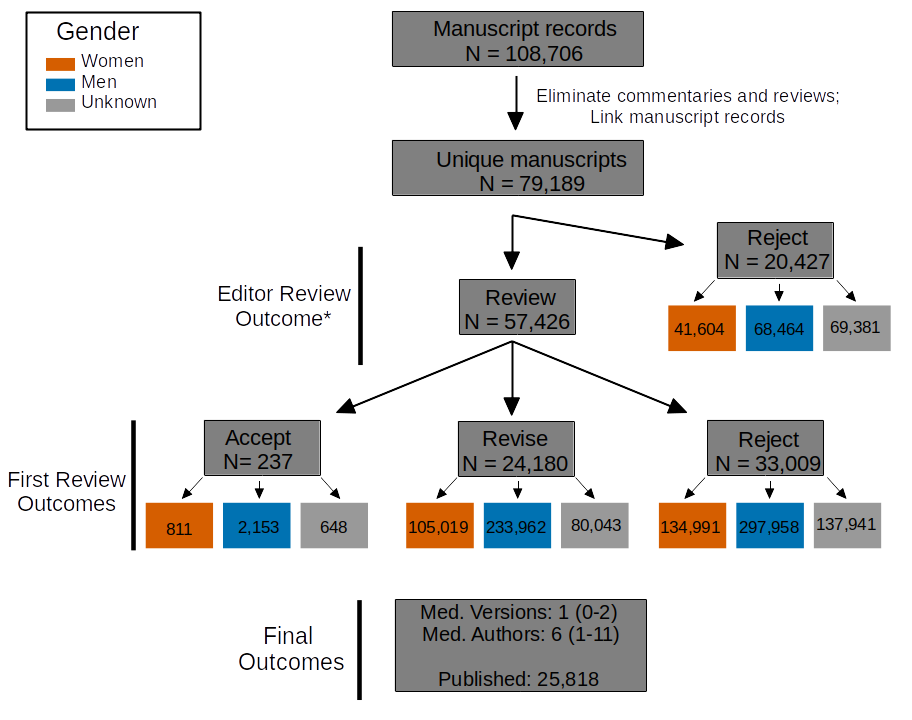
\includegraphics{population_diagram.png} \textbf{Figure 1. Overview of
manuscript outcomes.} Over 100,000 manuscript records were obtained for
the period between January 2012 and August 2018. After eliminating
non-primary research articles and linking records for resubmitted
articles, there were 81,897 unique manuscripts processed. The median
number of versions was 1 (iqr=1) with a median of 6 (iqr=5) authors per
manuscript. 34,196 of these were published as of August 2018. Over 1,000
of the manuscripts were accepted without revisions at their first
submission and there were 4,337 women (orange), 10,152 men (blue), and
3,037 unknown gendered individuals associated with their records (e.g.,
author, editor, reviewer). Revisions were requested for 26,016
manuscripts and 54,389 manuscripts were rejected at their first
submission.

\newpage

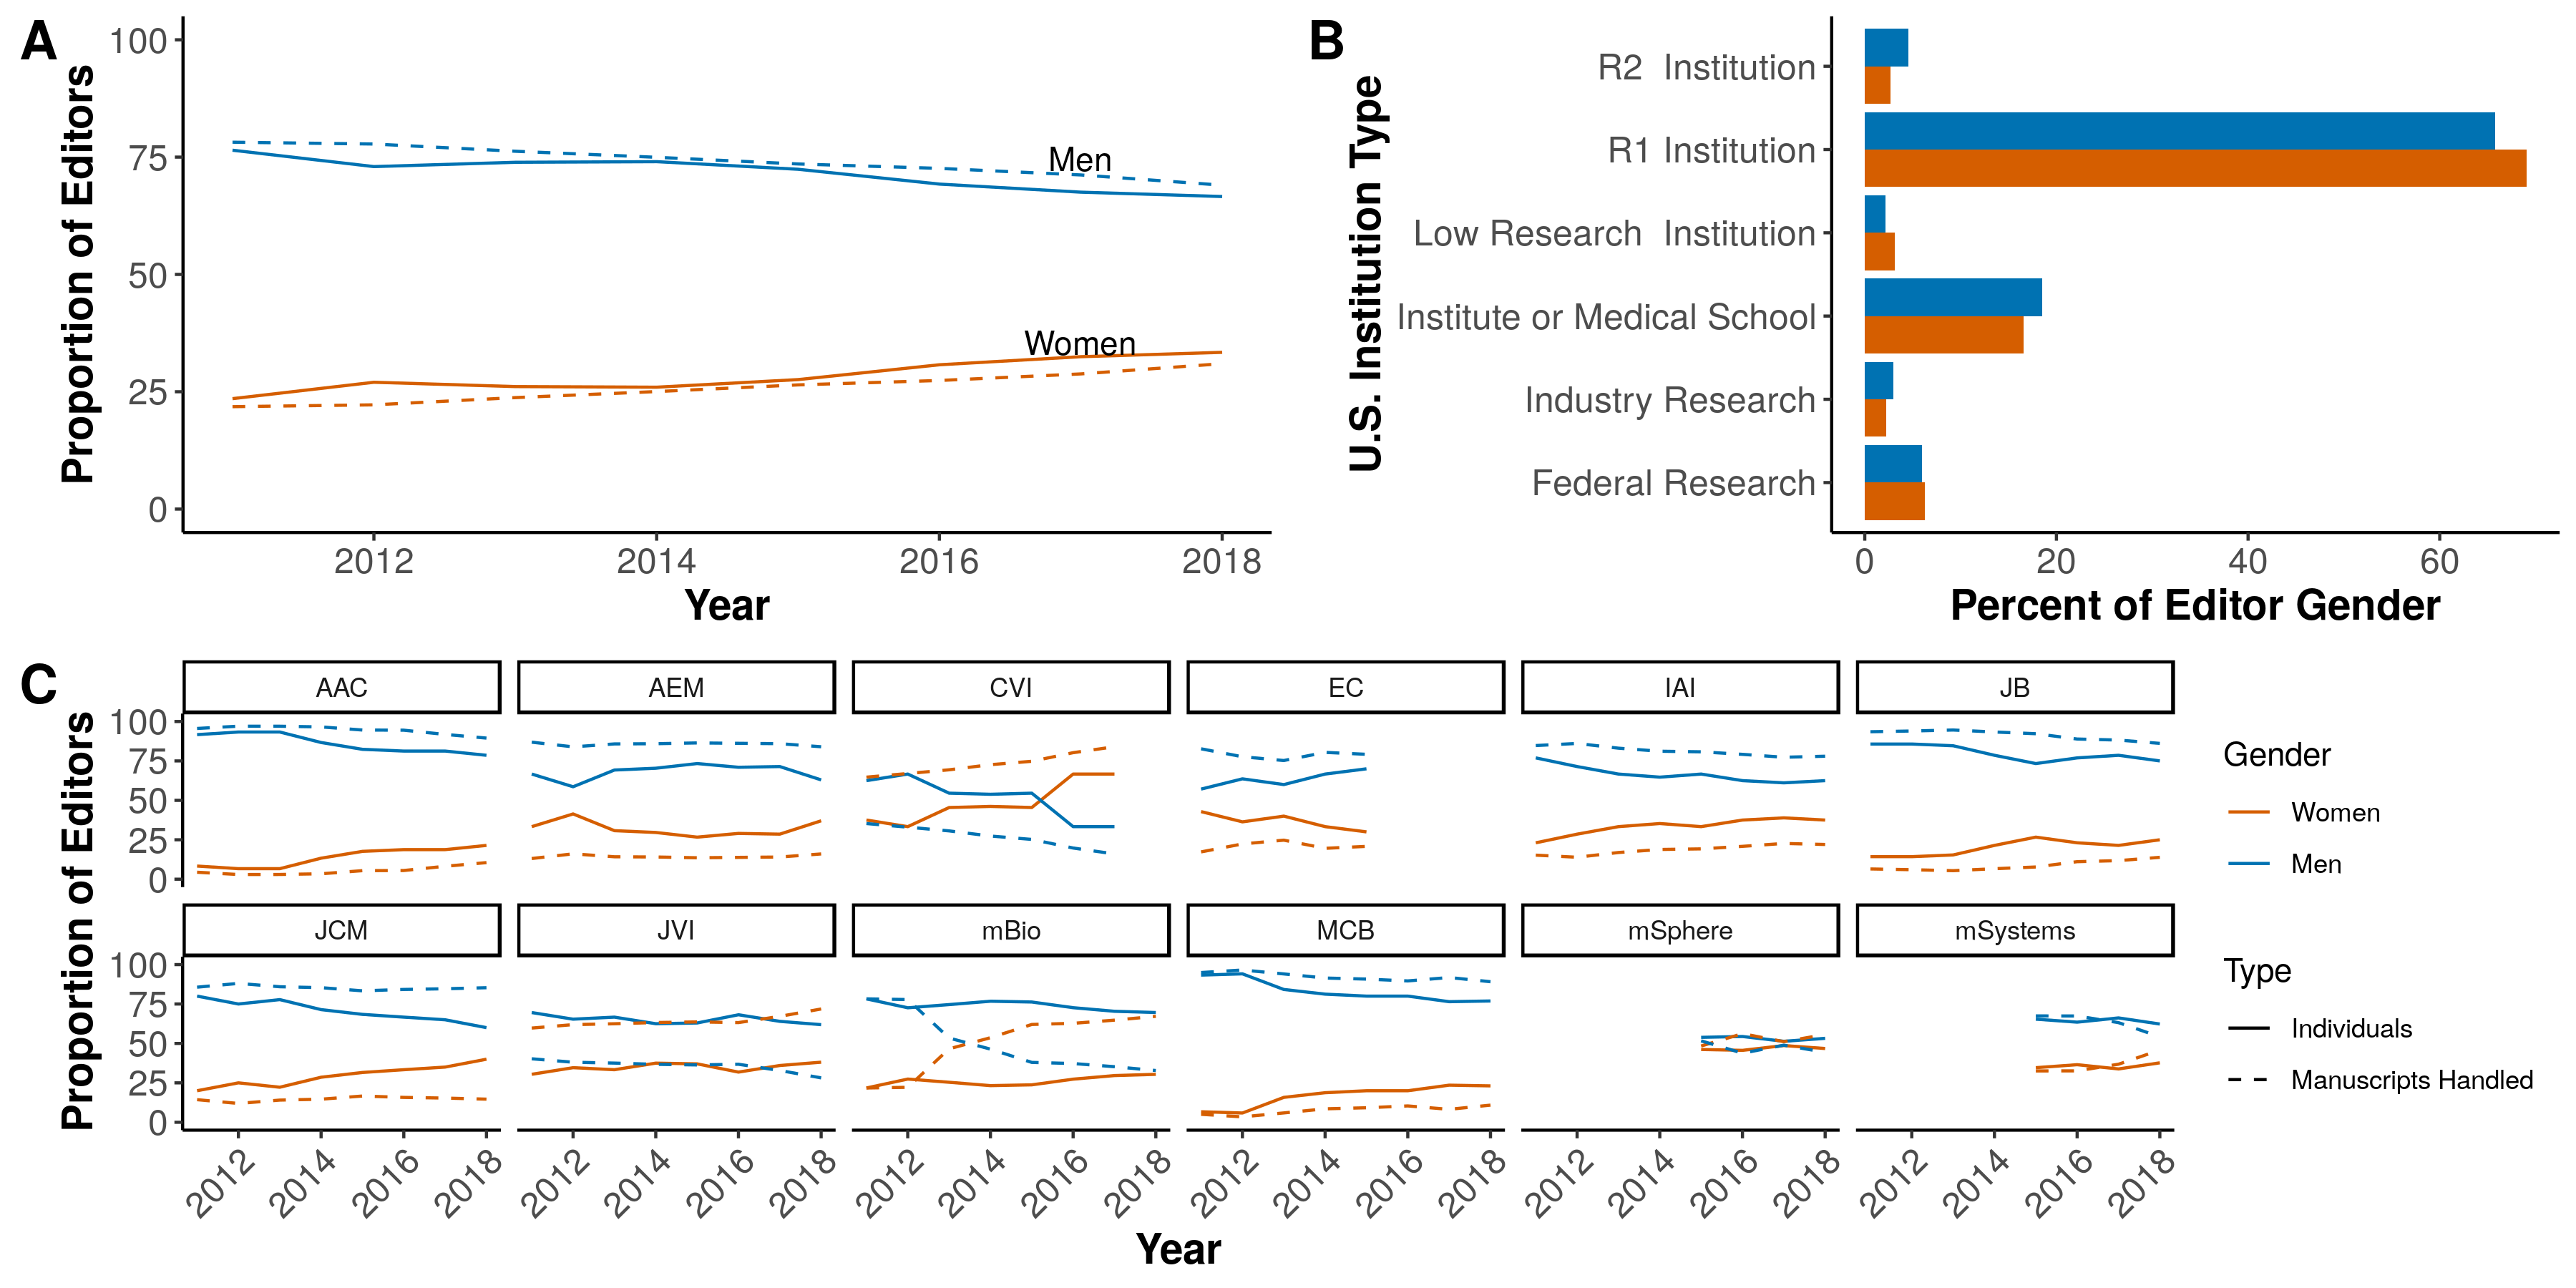
\includegraphics{Figure_1.png} \textbf{Figure 2. Gendered representation
among gatekeepers.} Proportion of editors from (A) institution types and
(B) over time from 2012 to 2018. Editors and senior editors are pooled
together. Proportion of reviewers from (C) institution types and (D)
over time from 2012 to 2018. (A,C) Each gender equals 100\% when all
instiutions are summed.(B,D) Each individual was counted once per
calendar year, proportions of each gender add to 100\% per year.

\newpage

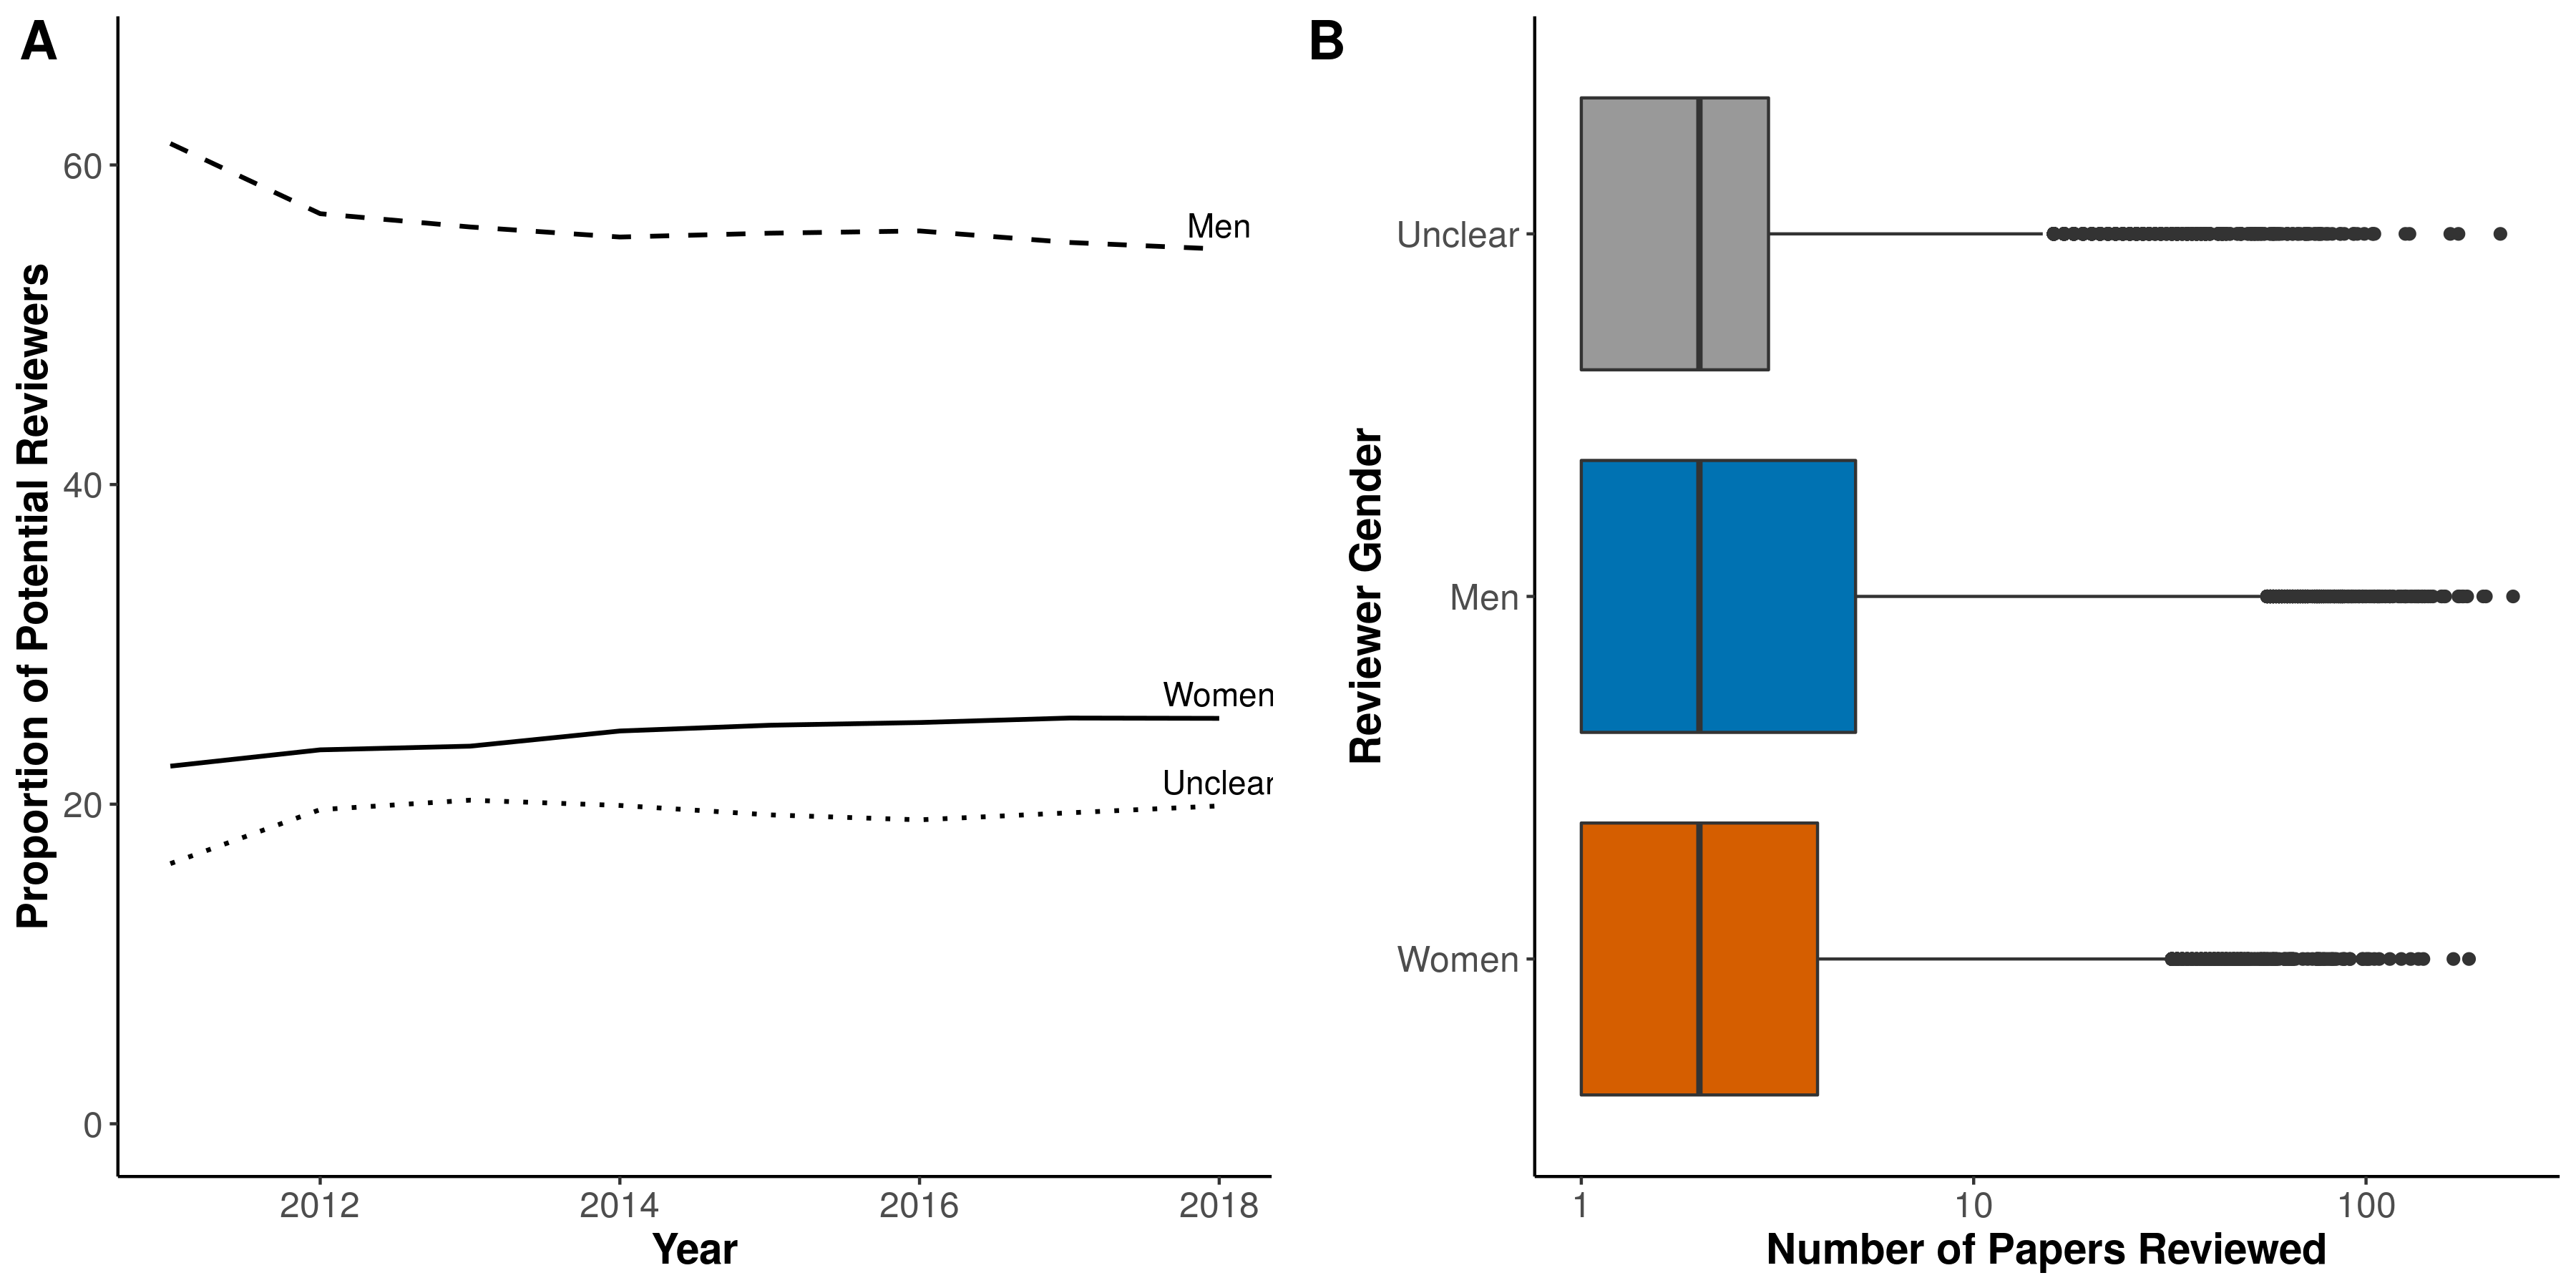
\includegraphics{Figure_2.png} \textbf{Figure 3. Gatekeeper workload and
response to requests to review.} (A) Proportion of manuscript workloads
by men and women editors, editorial rejections excluded. (B) Box plot
comparison of all manuscripts reviewed by individuals according to
gender. (C) The percent of reviewers by gender that either accepted the
opportunity to review or did not respond to a request to review, split
according to the editor's gender. (D) Percent of each potential reviewer
gender contacted to review, according to the editor's gender.

\newpage

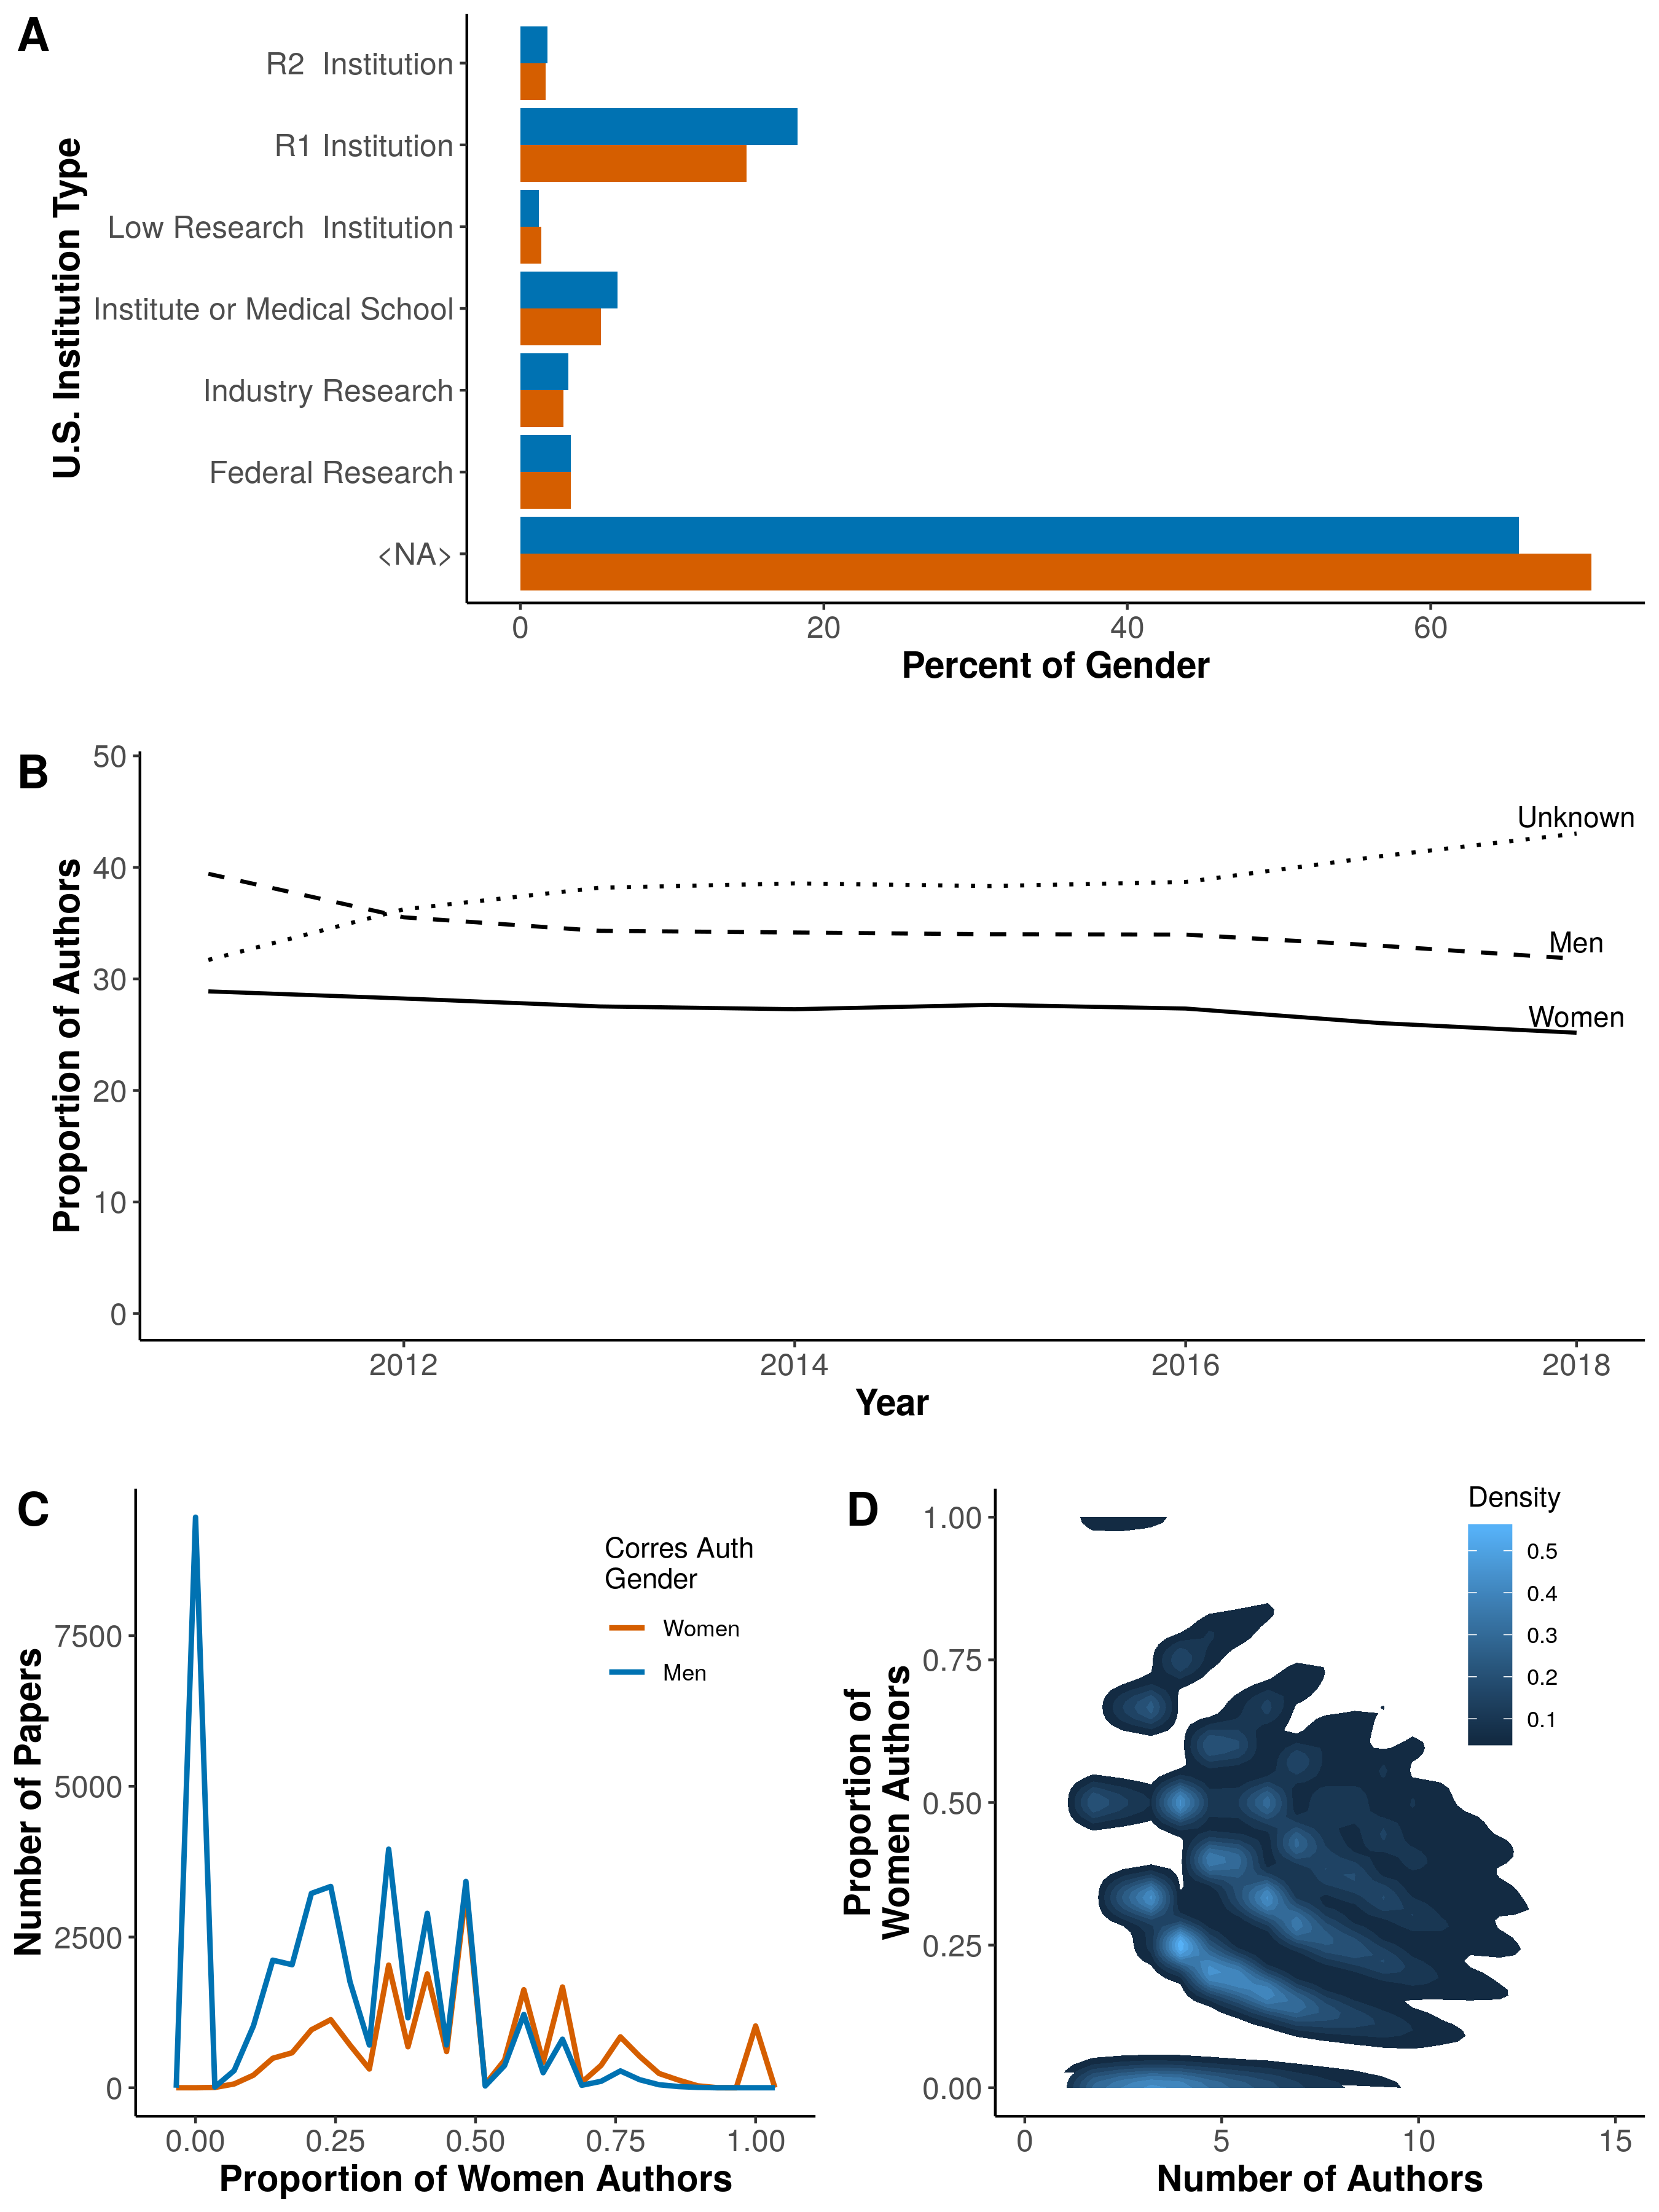
\includegraphics{Figure_3.png} \textbf{Figure 4. Author representation
by gender.} The proportion of (A) men and women authors from each
institution type, (B) men, women, and unknown authors from 2012 - 2018.
Each individual was counted once per calendar year. The proportion of
(C) first authors and (D) corresponding authors from 2012 - 2018 on
submitted (dashed) and published (solid) manuscripts.

\newpage

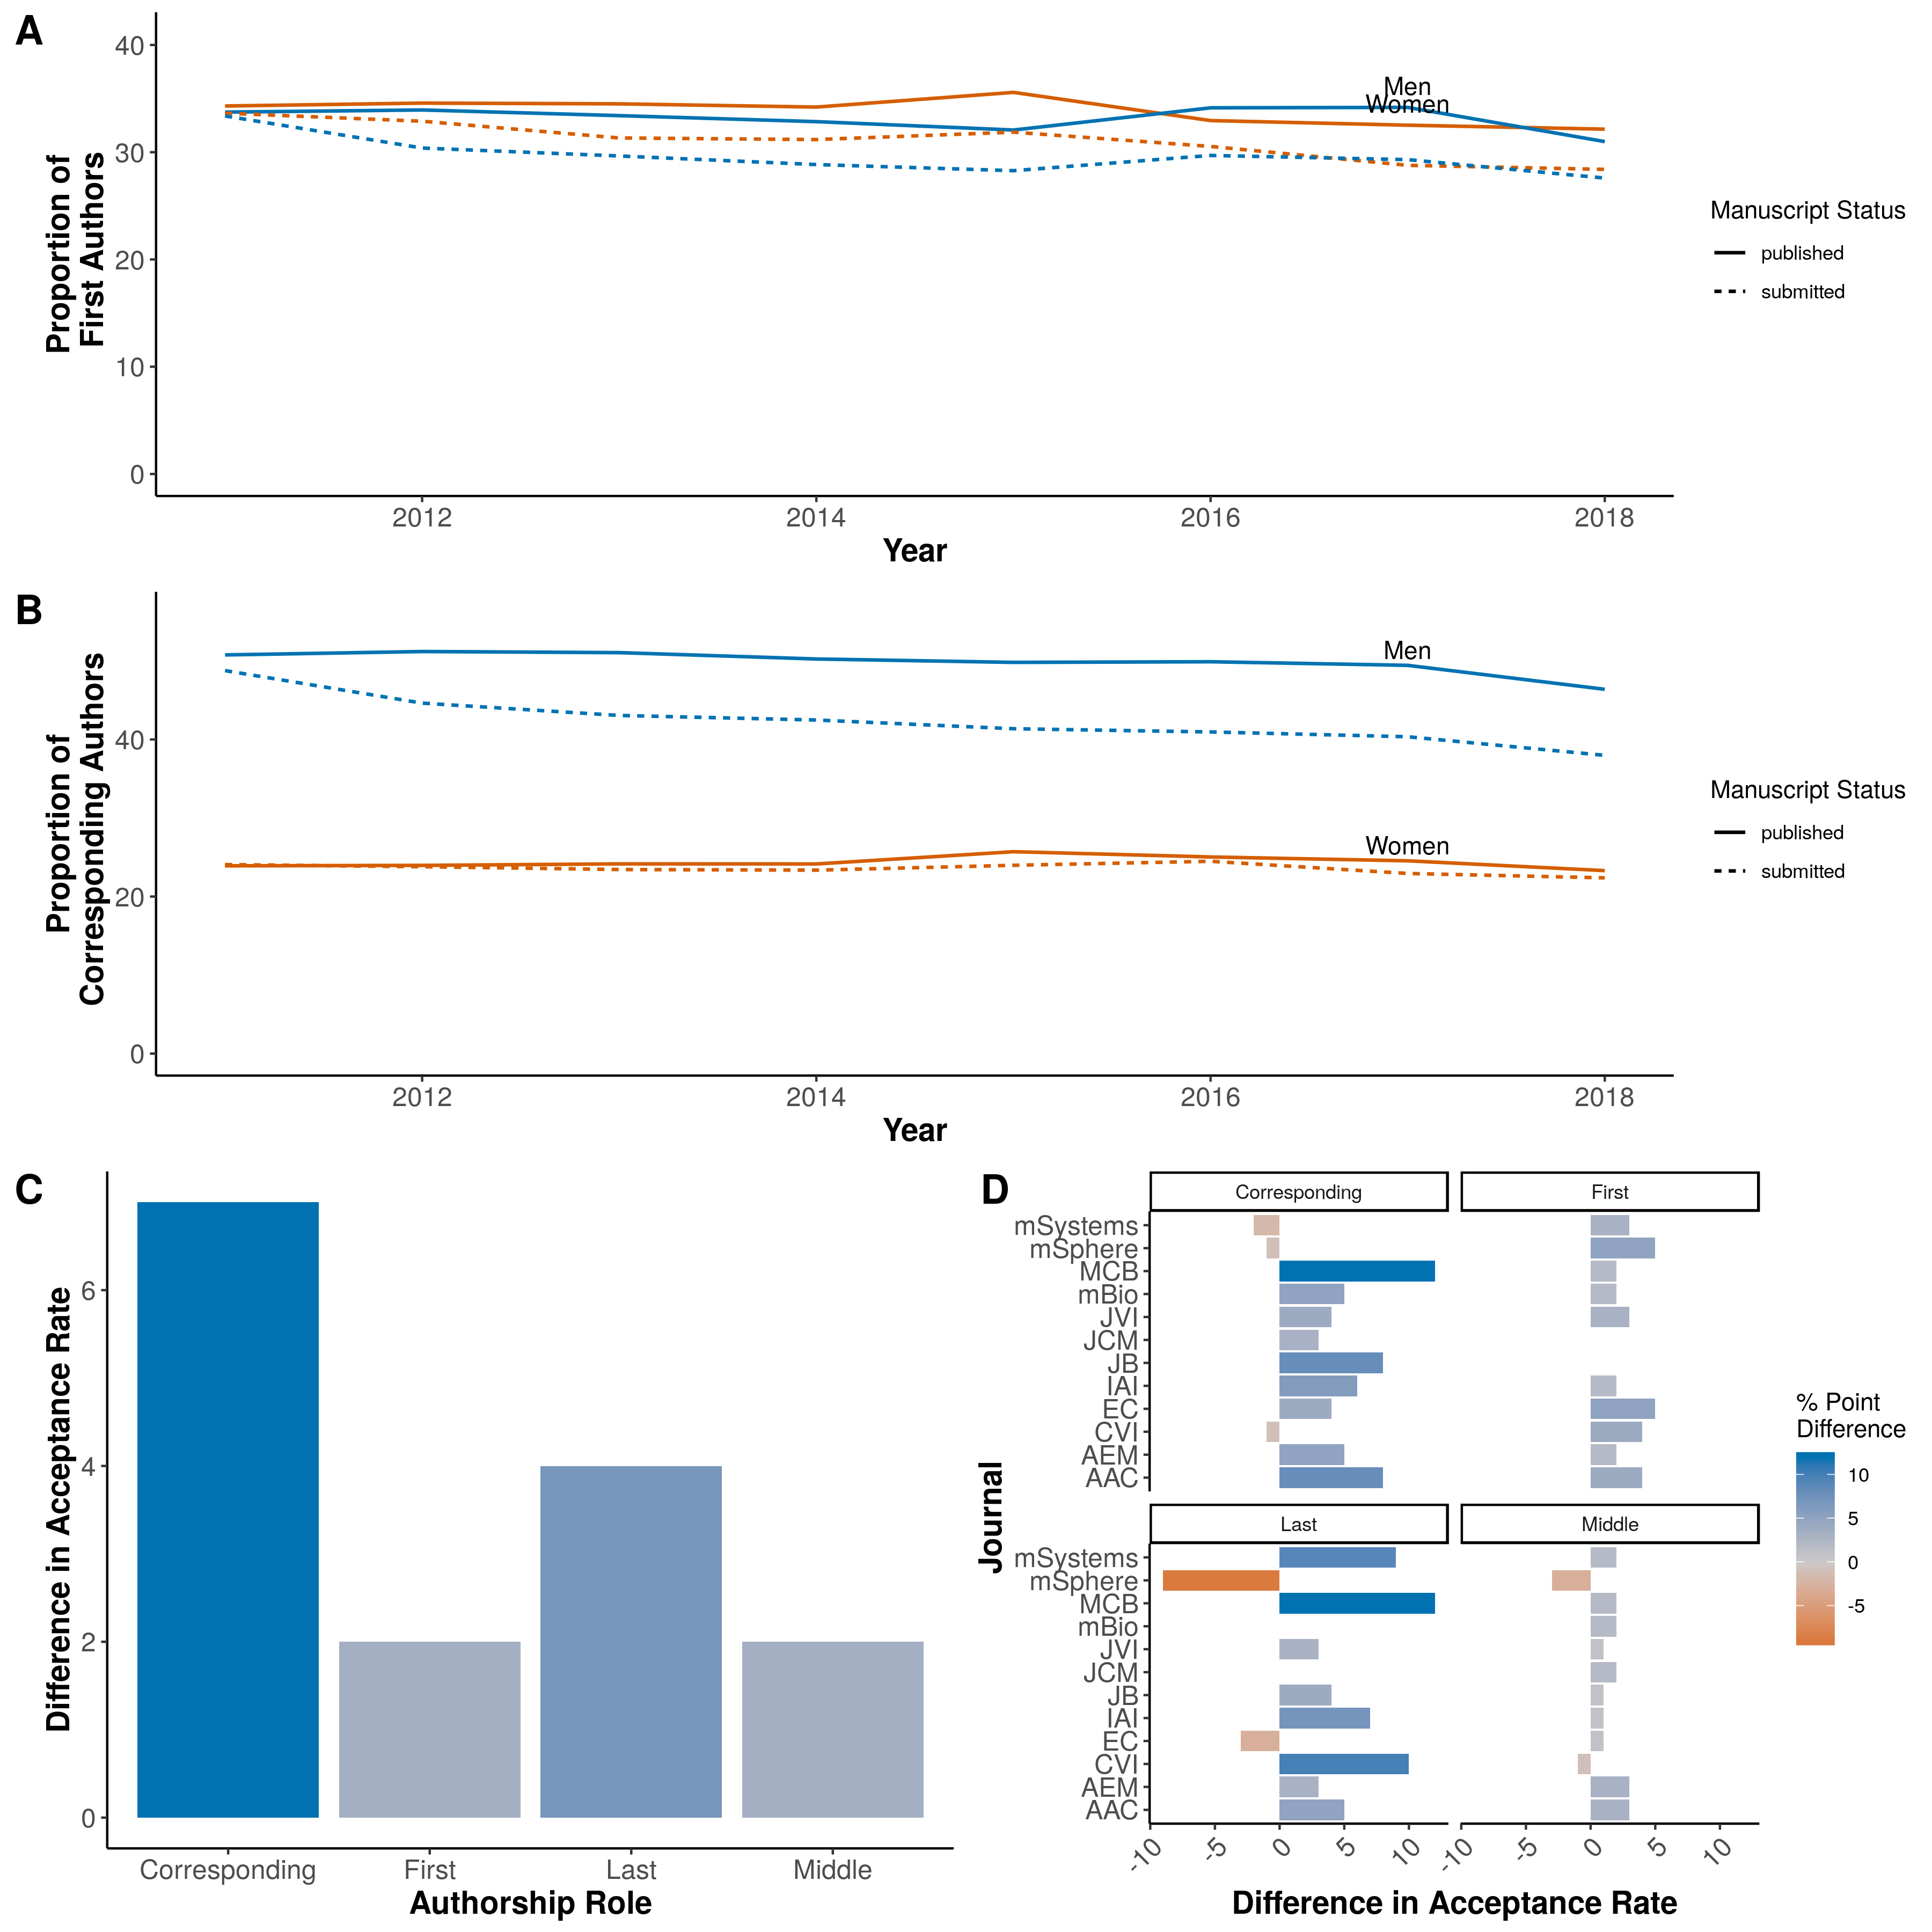
\includegraphics{Figure_4.png} \textbf{Figure 5. Difference in rejection
rates by corresponding author gender.} The percent of manuscripts
rejected by author gender and type (e.g., corresponding, first, last,
middle) at (A) all journals combined where 0 corresponds to equal rates
of rejection (the variation from parity is shown). (B) The difference in
percent editorial rejection rates for corresponding authors at each
journal, vertical line indicates the difference for all journals
combined. (D) The difference in percentage points between each decision
type for corresponding authors following the first peer review, vertical
lines indicate the difference value for all journals combined. Absence
of a bar indicates parity.

\newpage

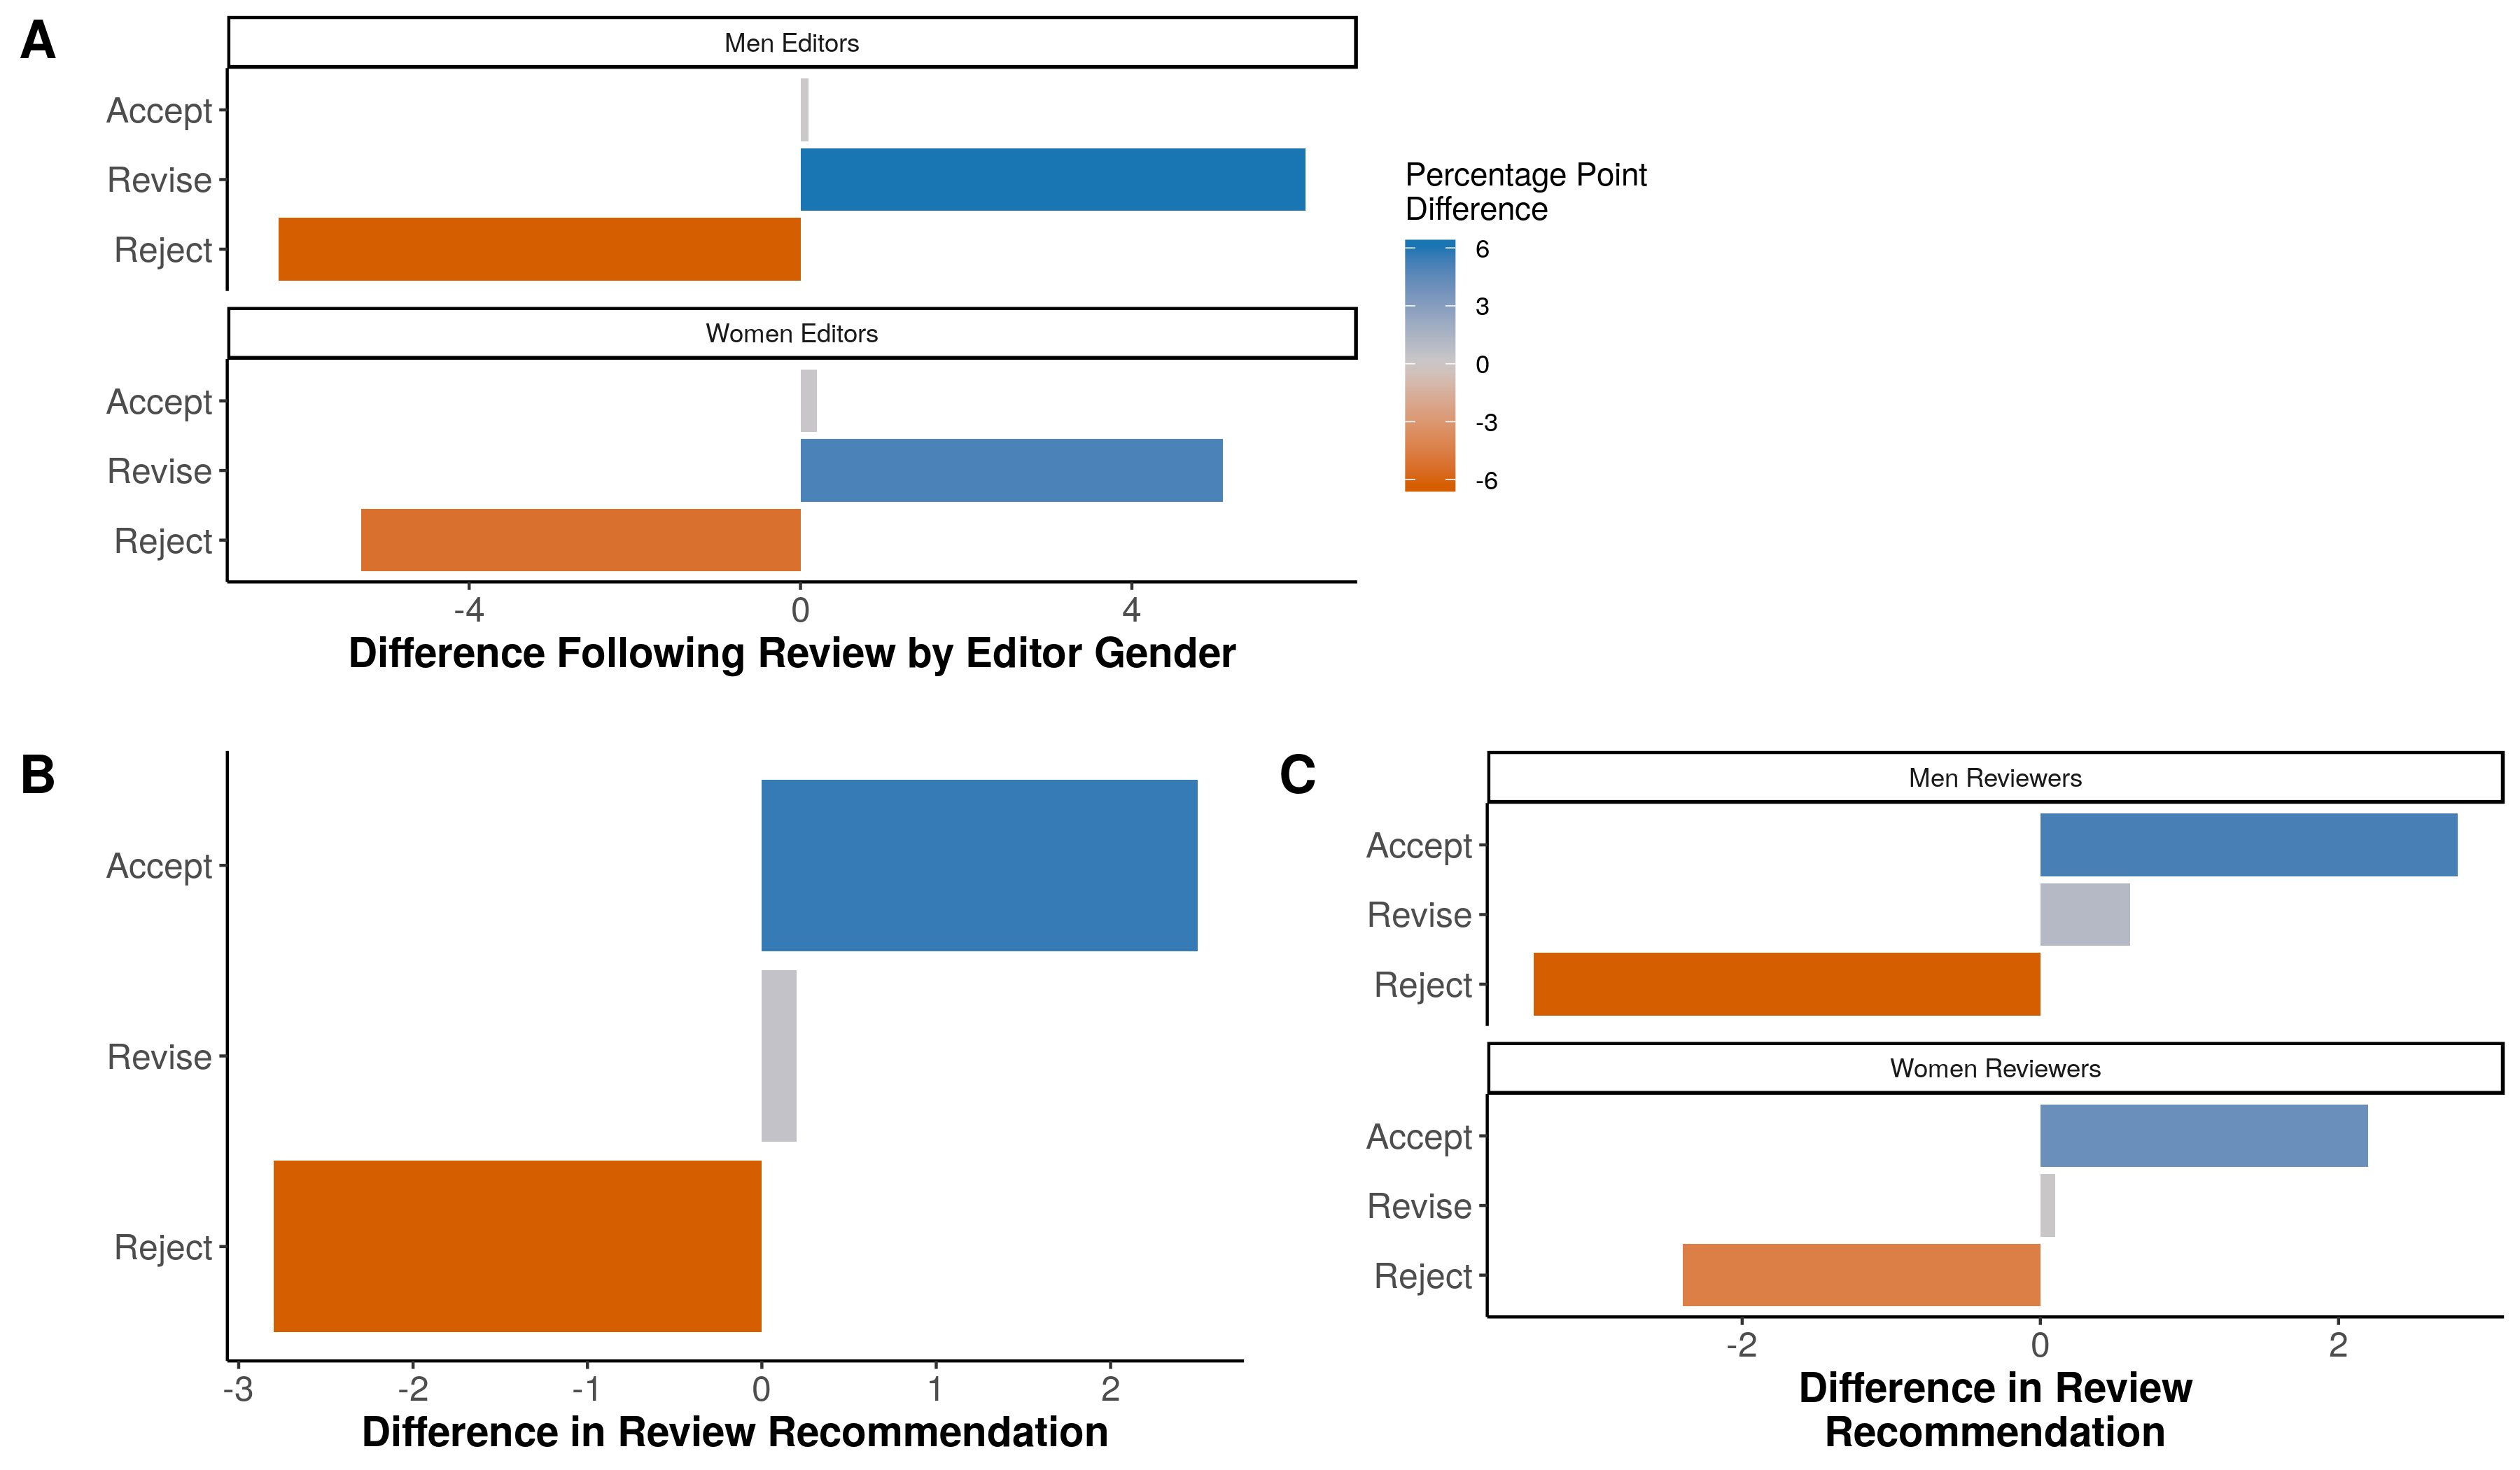
\includegraphics{Figure_5.png} \textbf{Figure 6. Difference in decisions
or recomendations according to the gatekeeper gender.} (A) Effect of
editor gender on the difference in percentage points for decisions
following review. (B) Difference in percentage points for review
recommendations and (C) how that is affected by reviewer gender. (A-C)
All journals combined.

\newpage

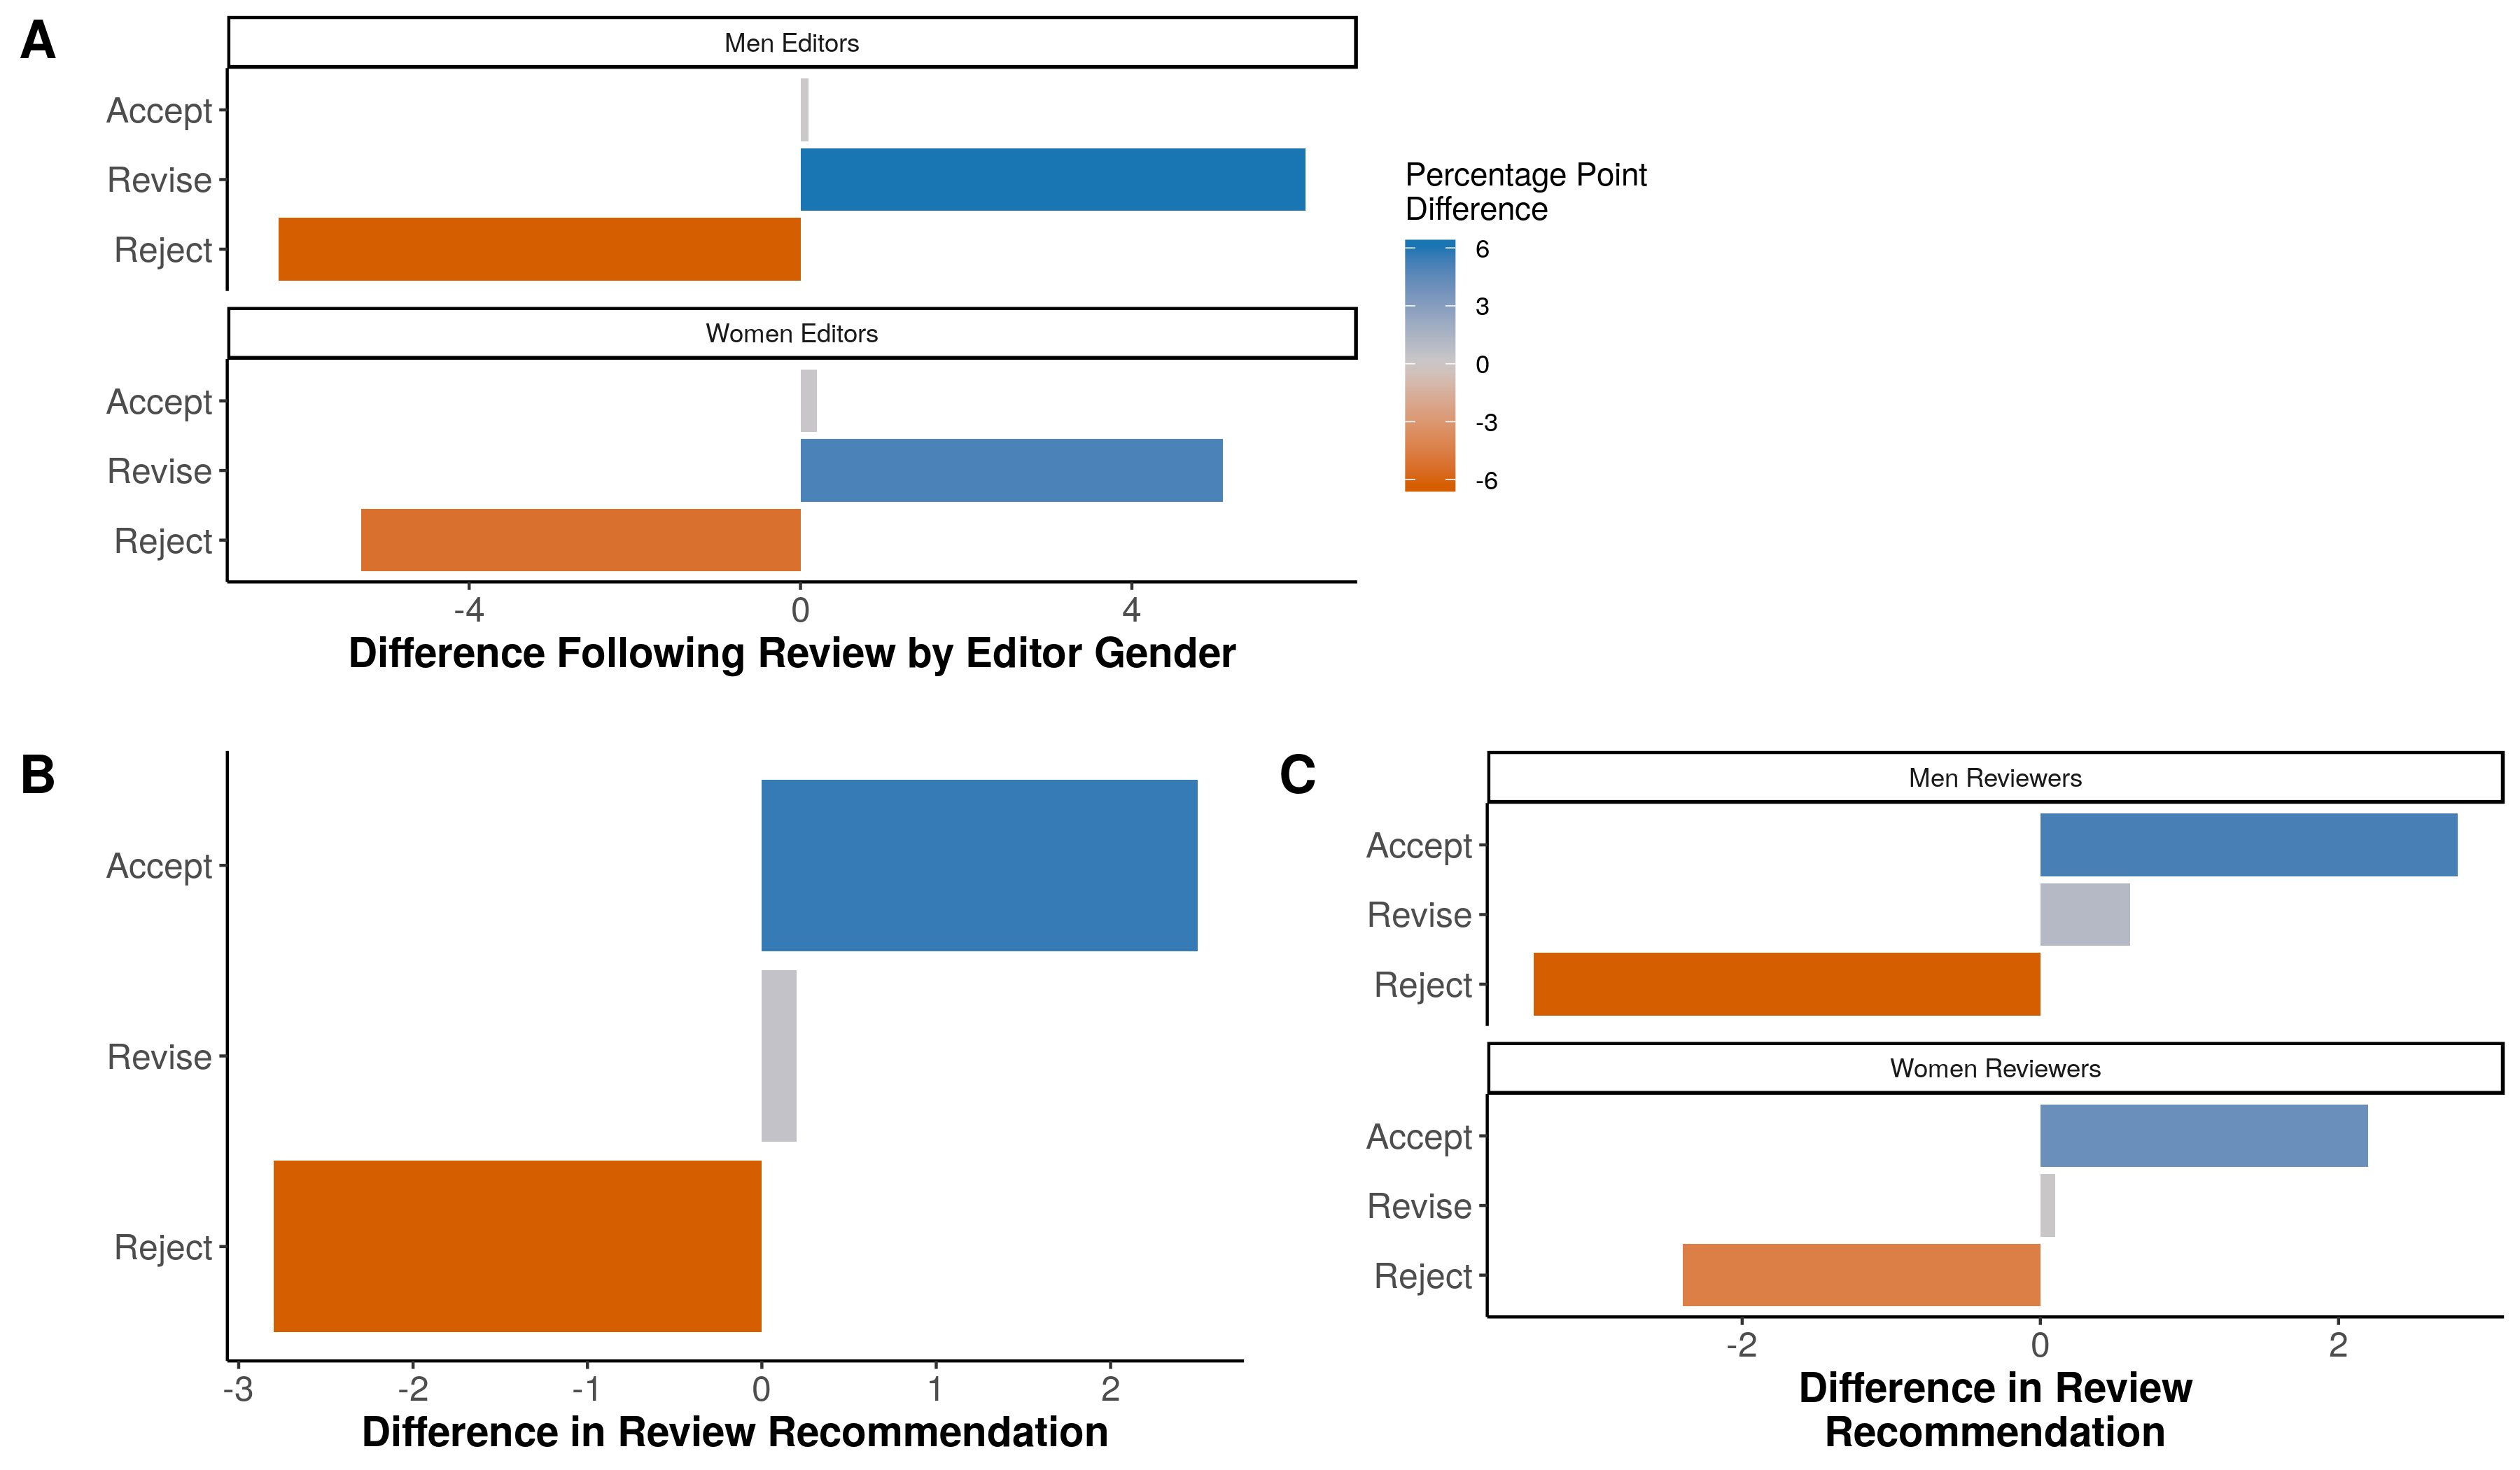
\includegraphics{Figure_6.png} \textbf{Figure 7. Impact of origin and
U.S. institution type on manuscript decisions by gender.} Difference in
percentage points for (A) editorial rejections and (B) following first
review of manuscripts submitted by US-based corresponding authors.
Vertical line indicates value for all ASM journals combined. (C)
Difference in percentage points for acceptance and editorial rejections
according to institution types and (D) acceptance decisions by to editor
gender and institution types.

\newpage

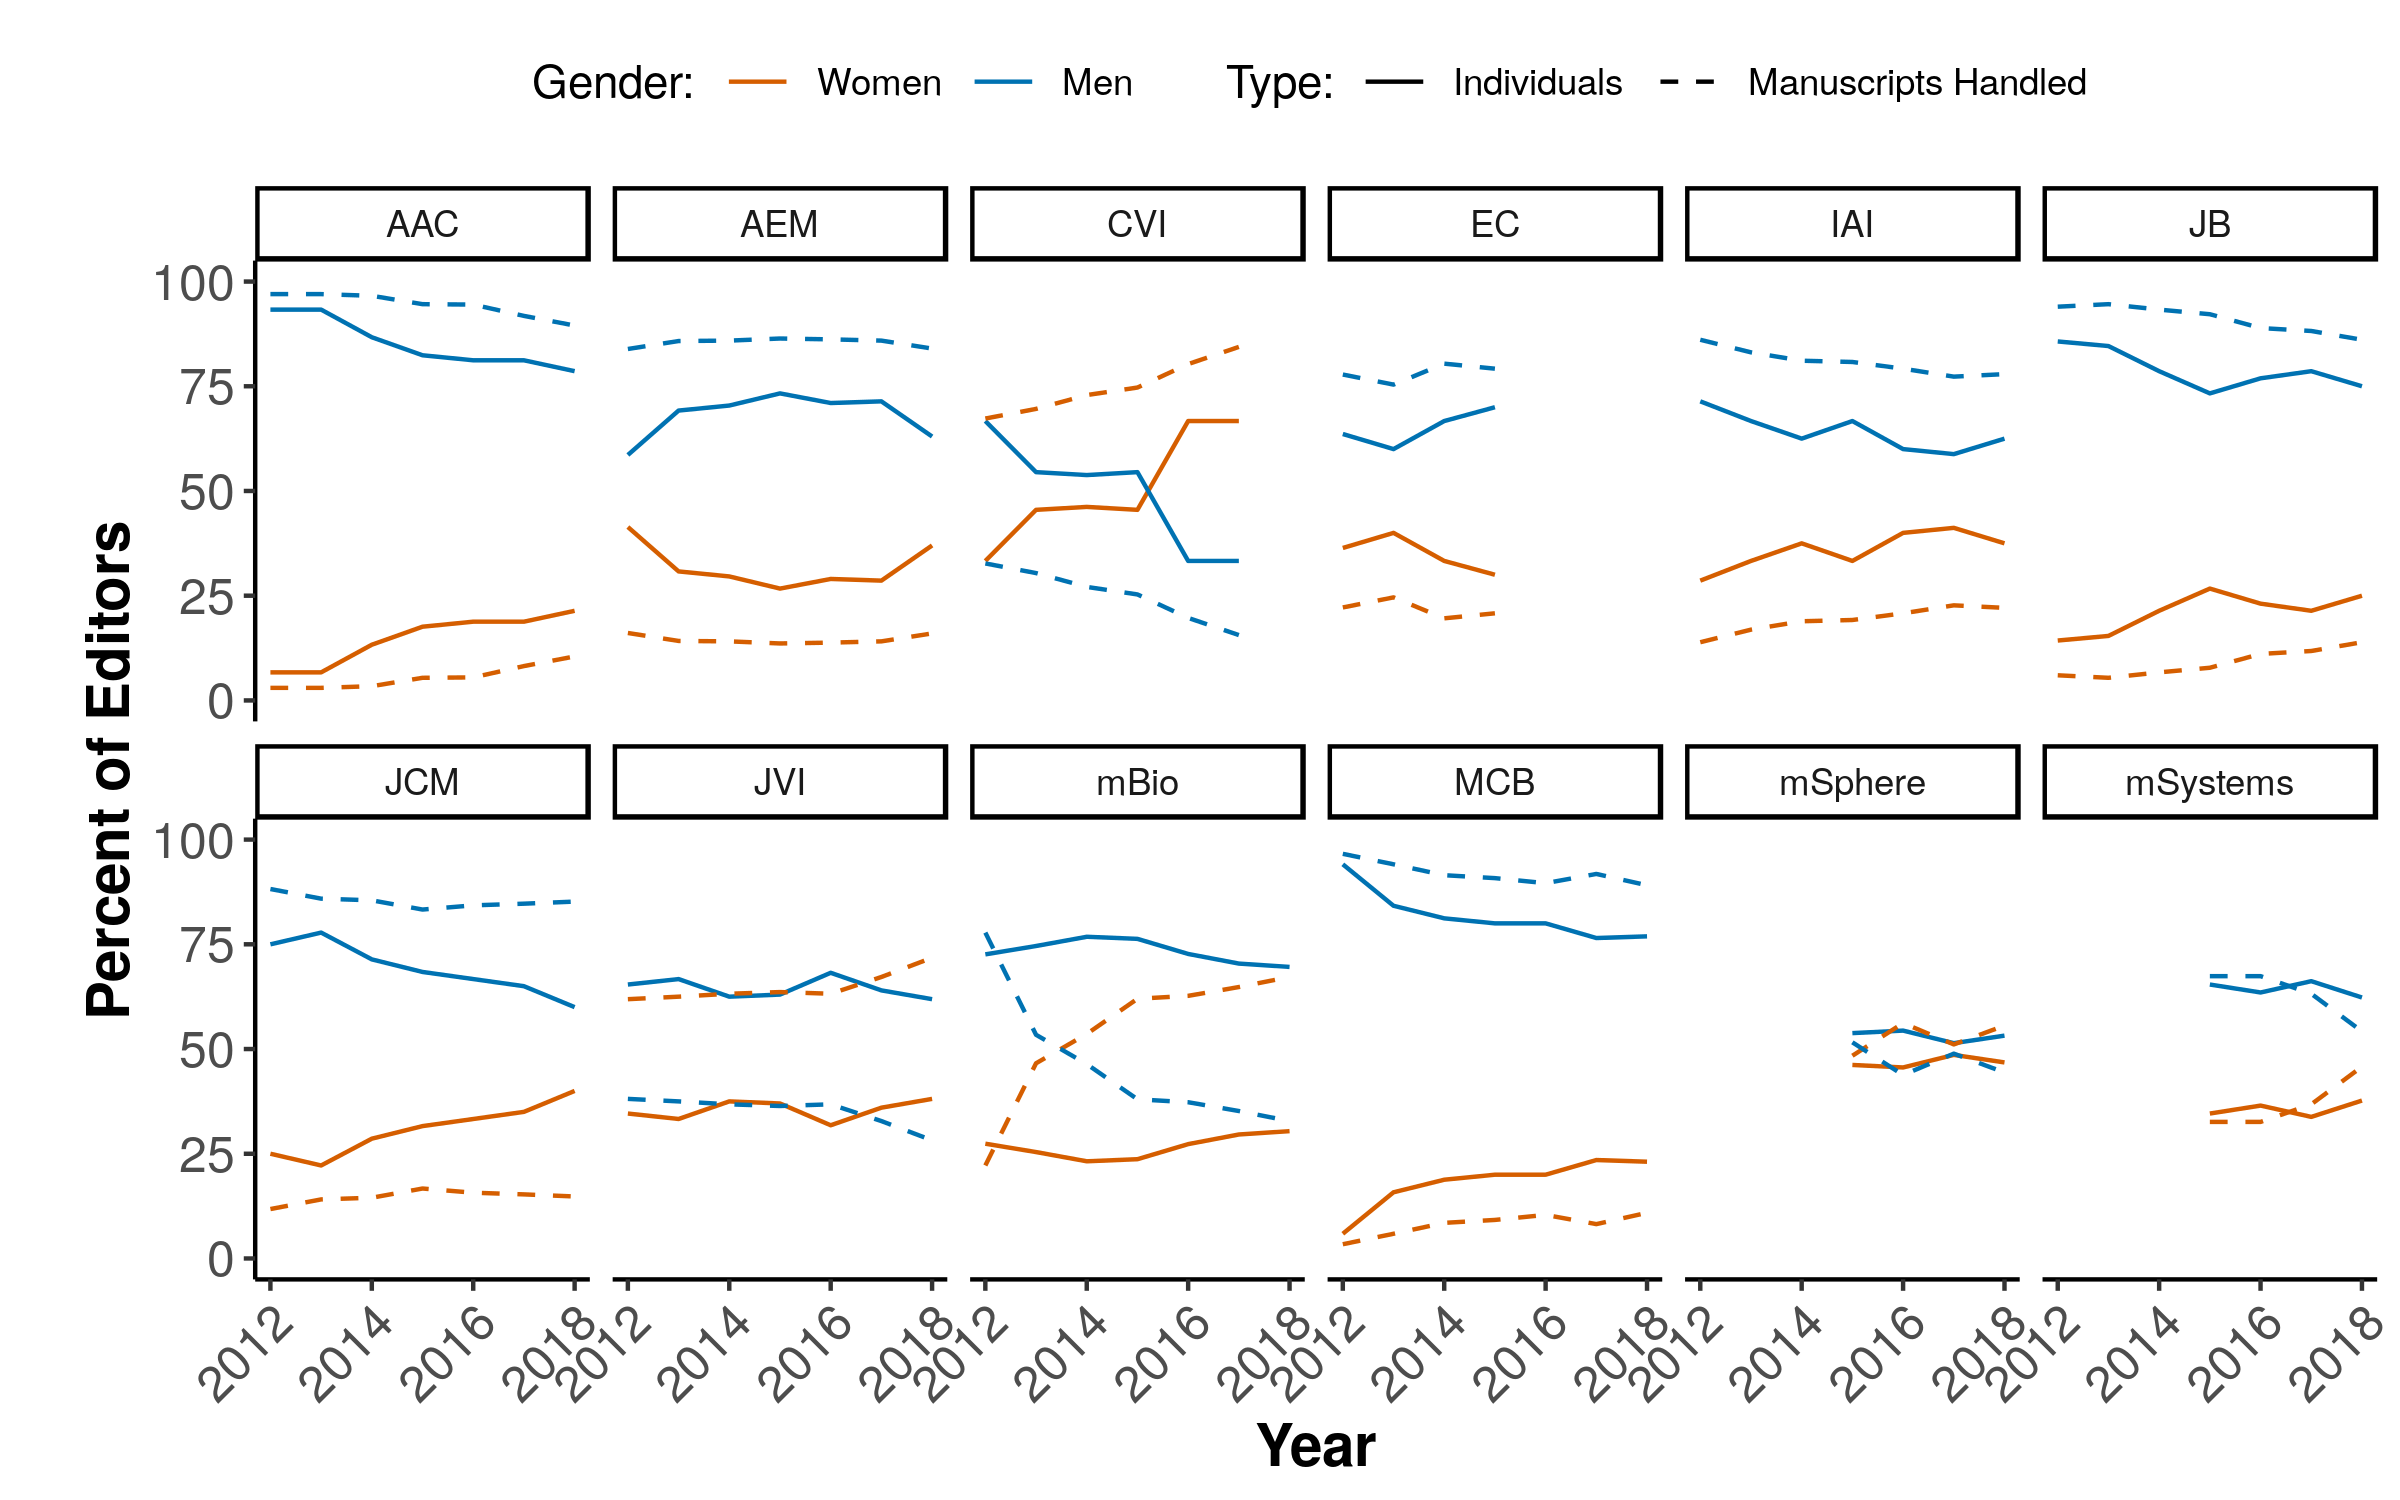
\includegraphics{Figure_S1.png} Figure S1. The proportion of editors
(solid line) and their workloads (dashed line) at each ASM journal from
2012 to 2018.

\newpage

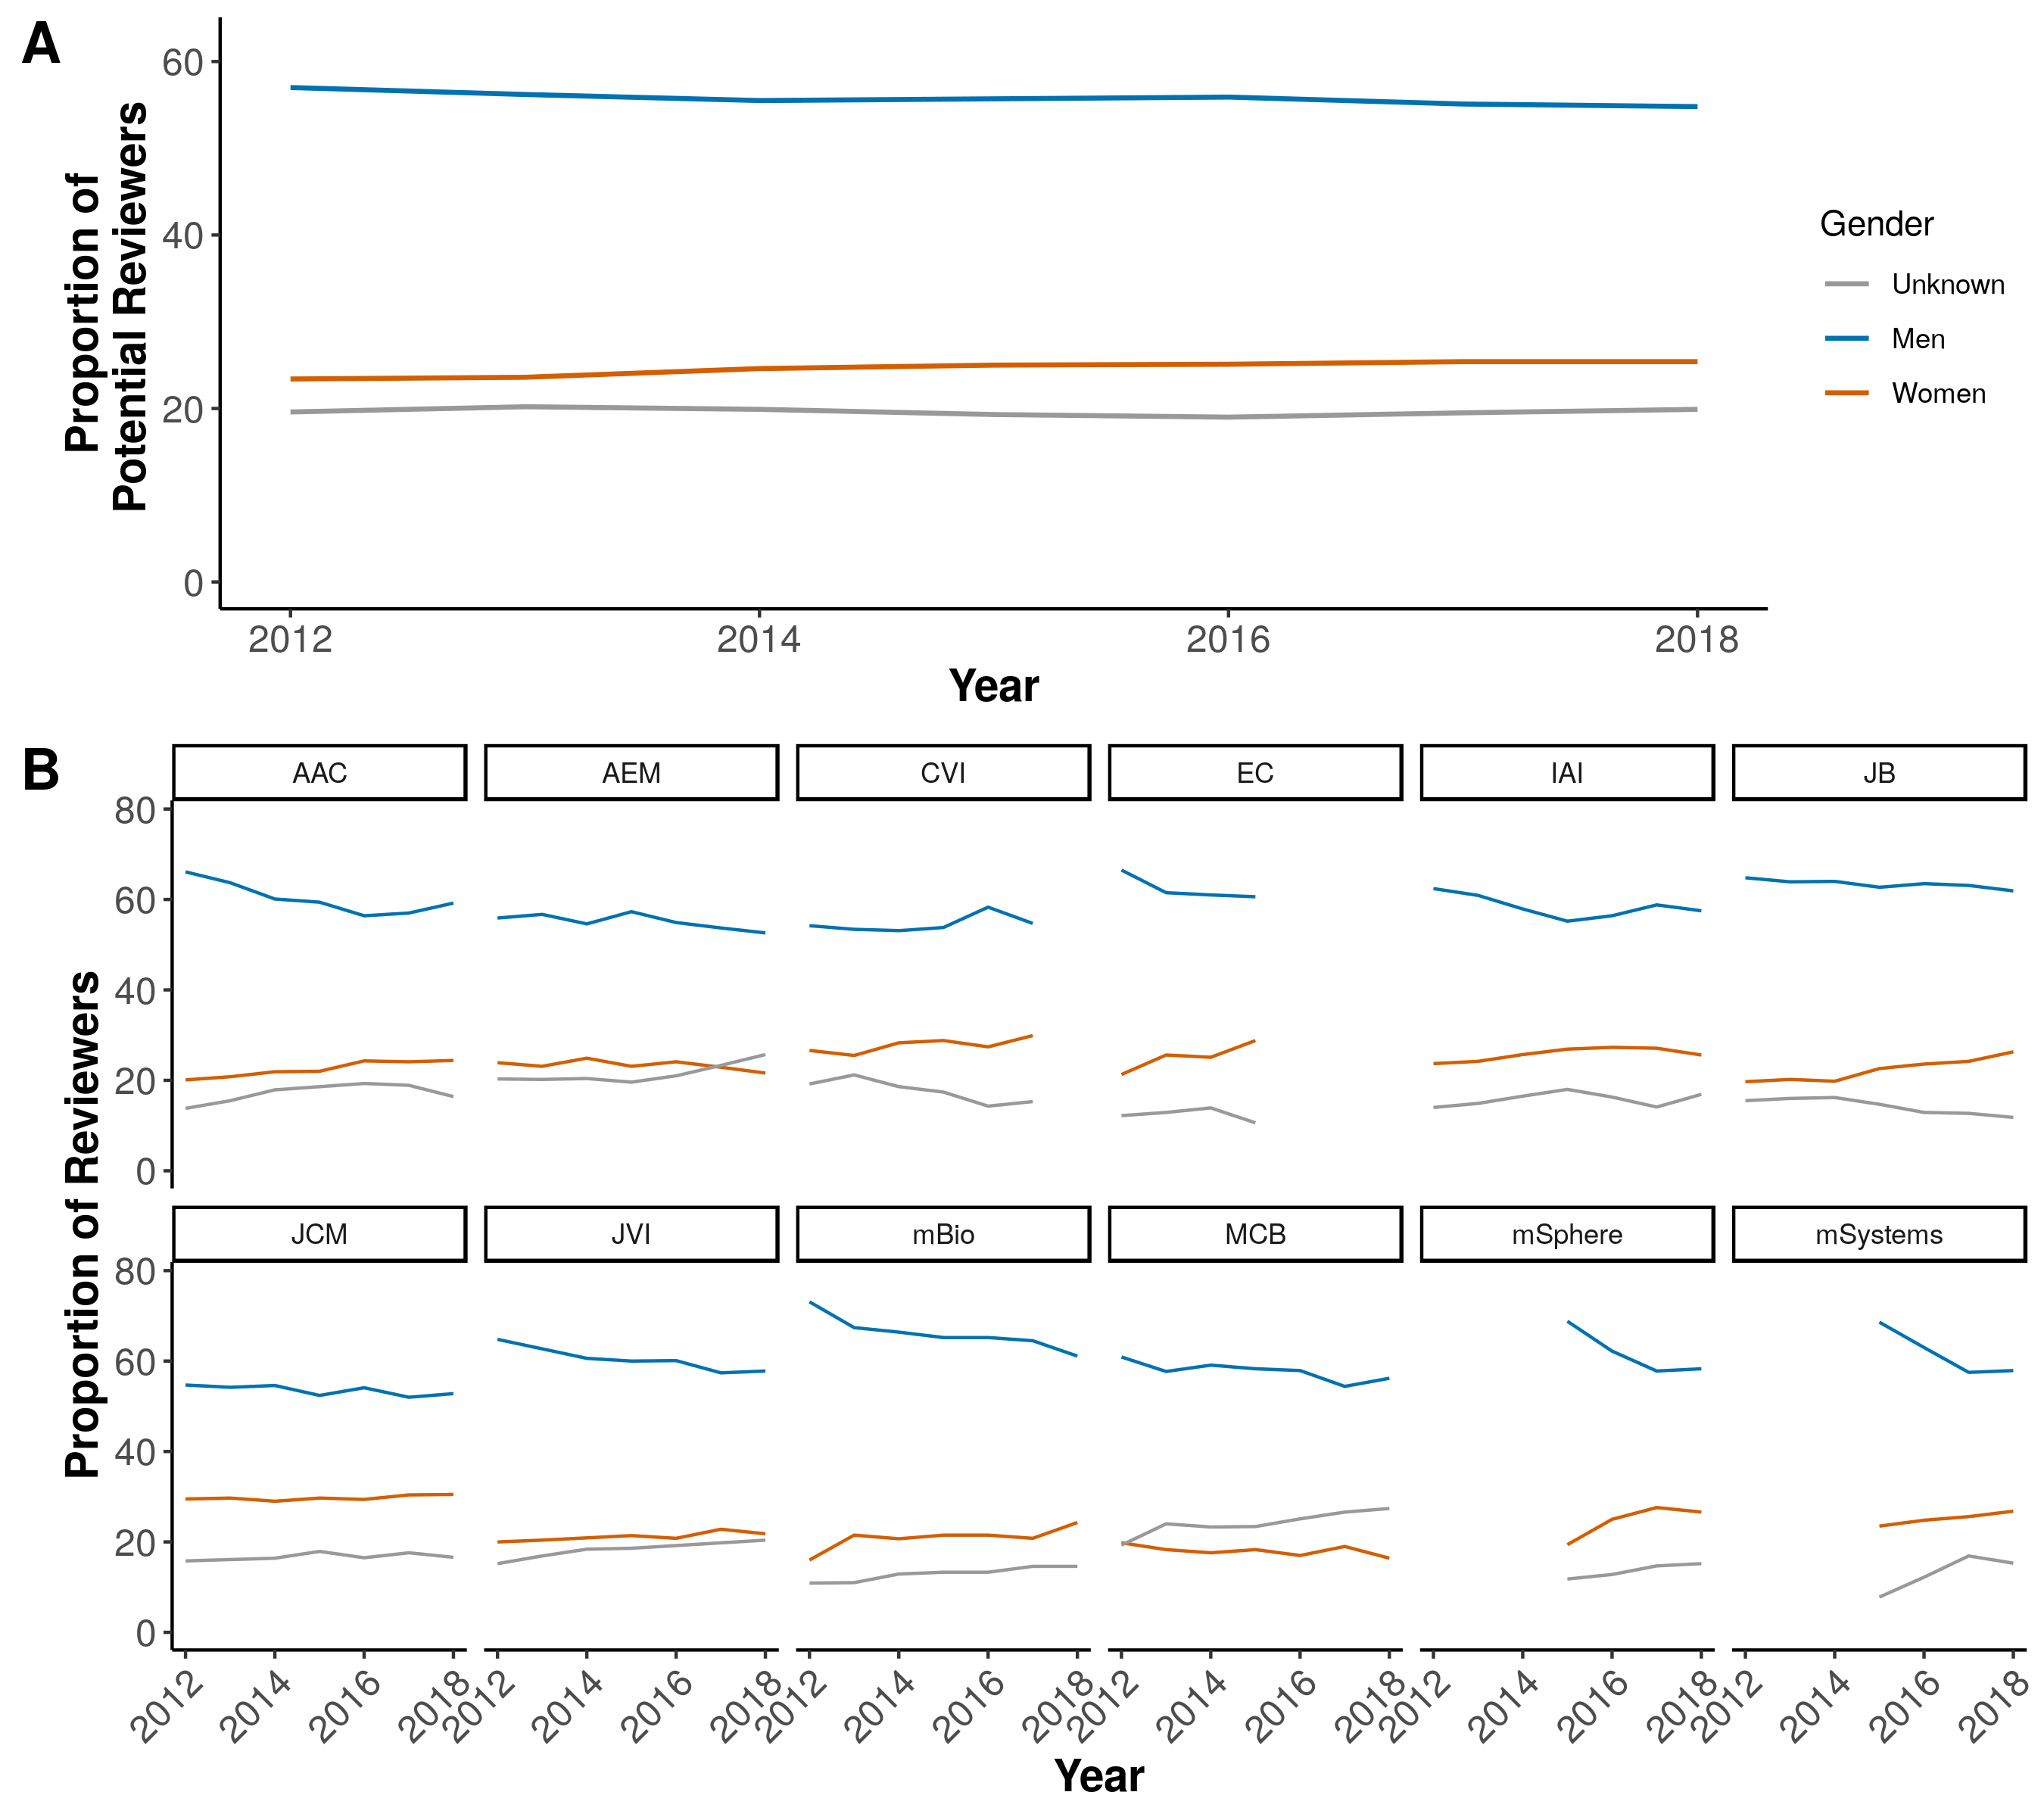
\includegraphics{Figure_S2.png} Figure S2. The proportion of (A)
potential reviewers at all ASM journals combined, (B) reviewers at each
ASM journal.

\newpage

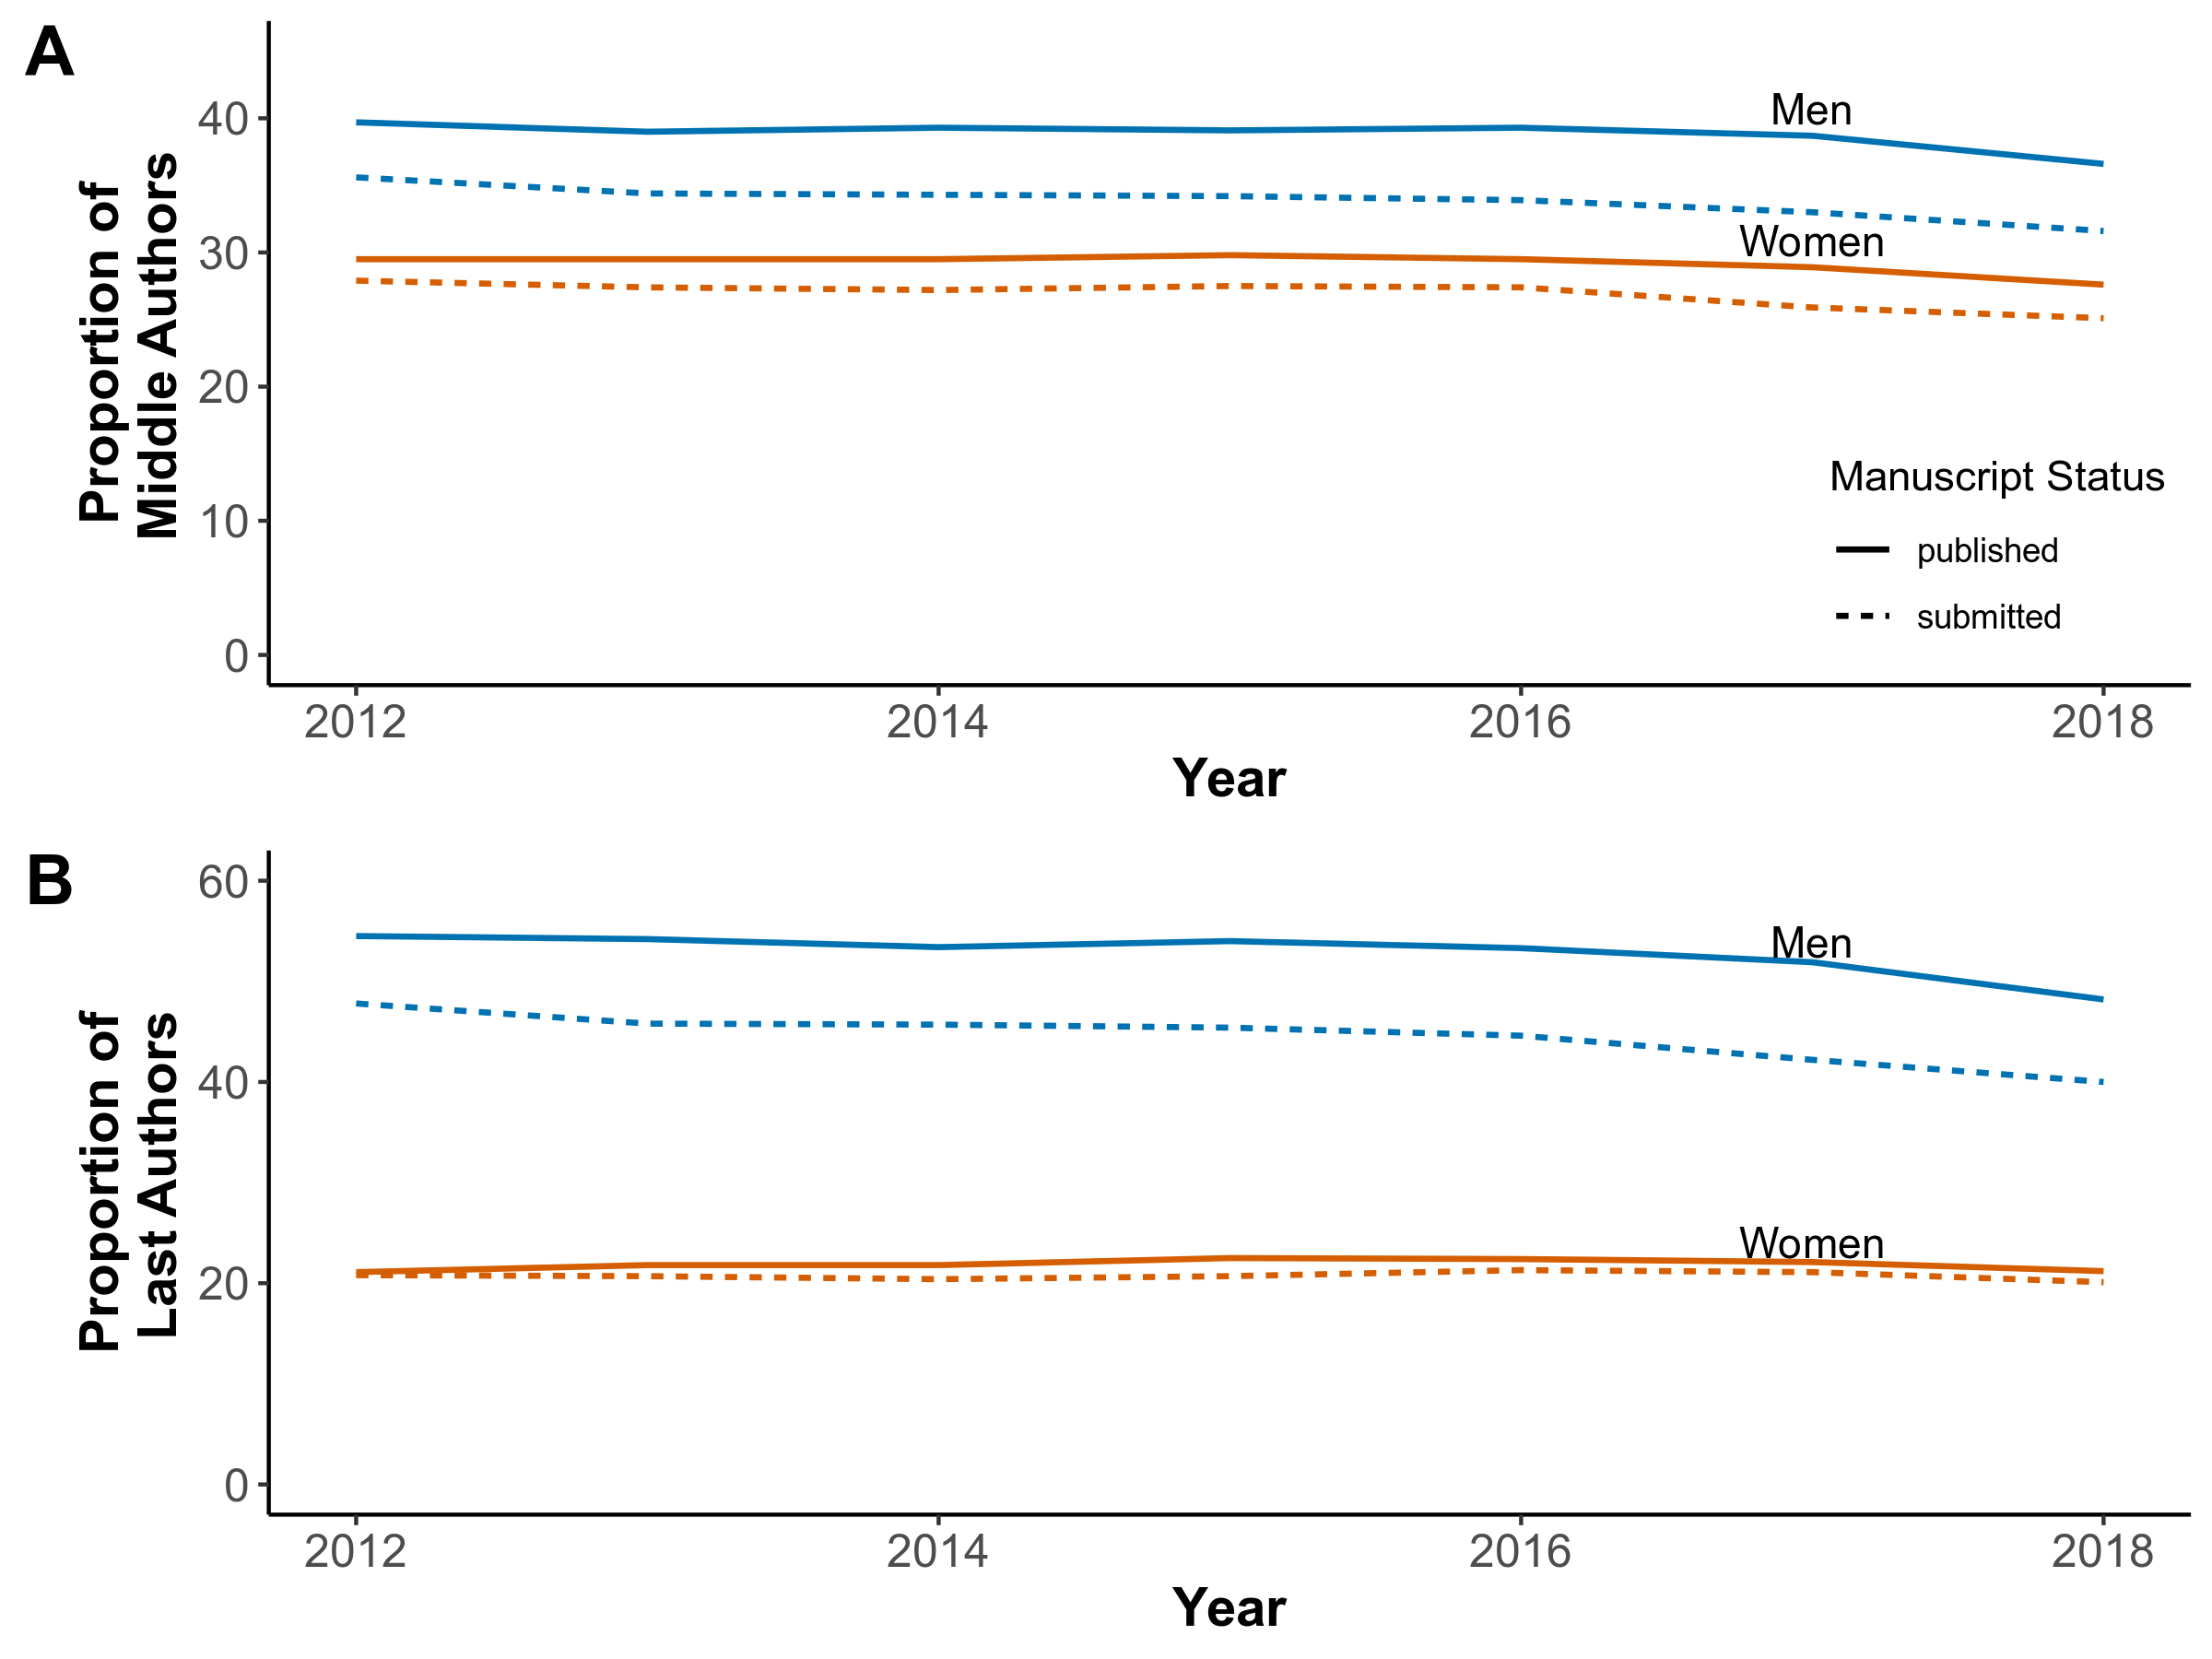
\includegraphics{Figure_S3.png} Figure S3. The proportion of all
submitting (dashed line) and publishing (solid line) (A) middle and (B)
last authors by gender at each ASM journal.

\newpage

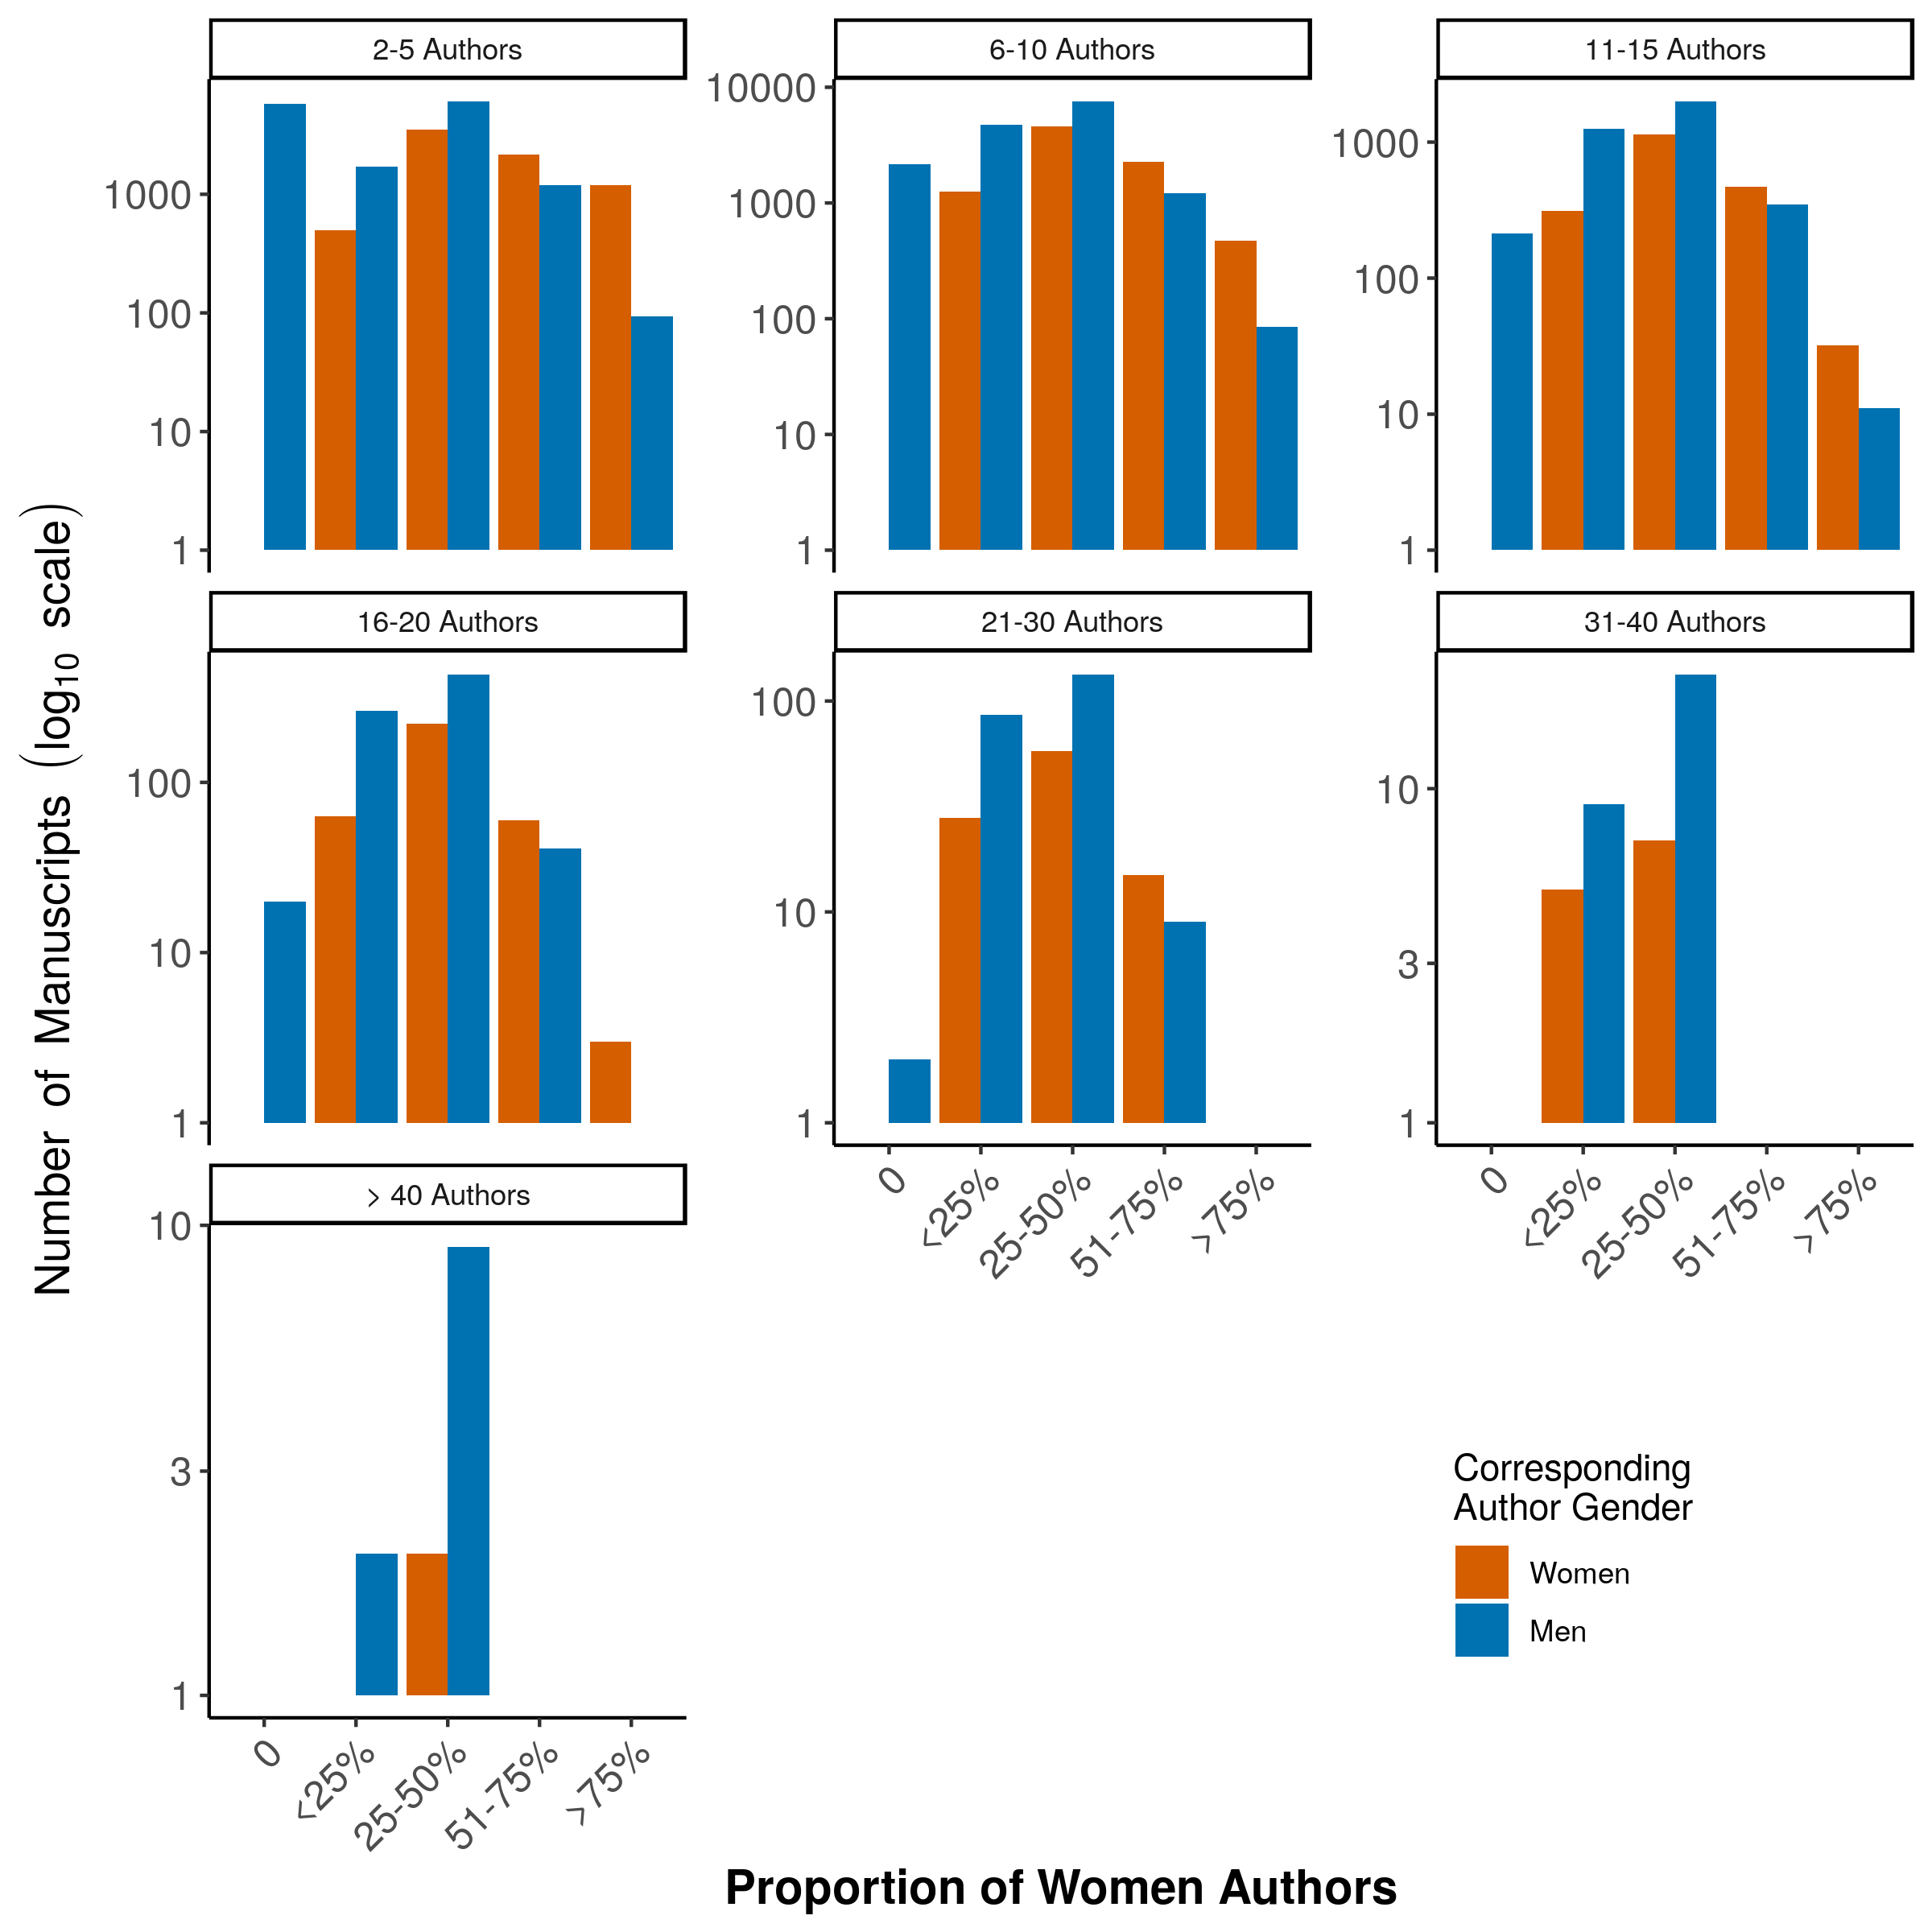
\includegraphics{Figure_S4.png} Figure S4. The proportion of women
authors on submitted manuscripts according to the number of authors and
the gender of the corresponding author.

\newpage

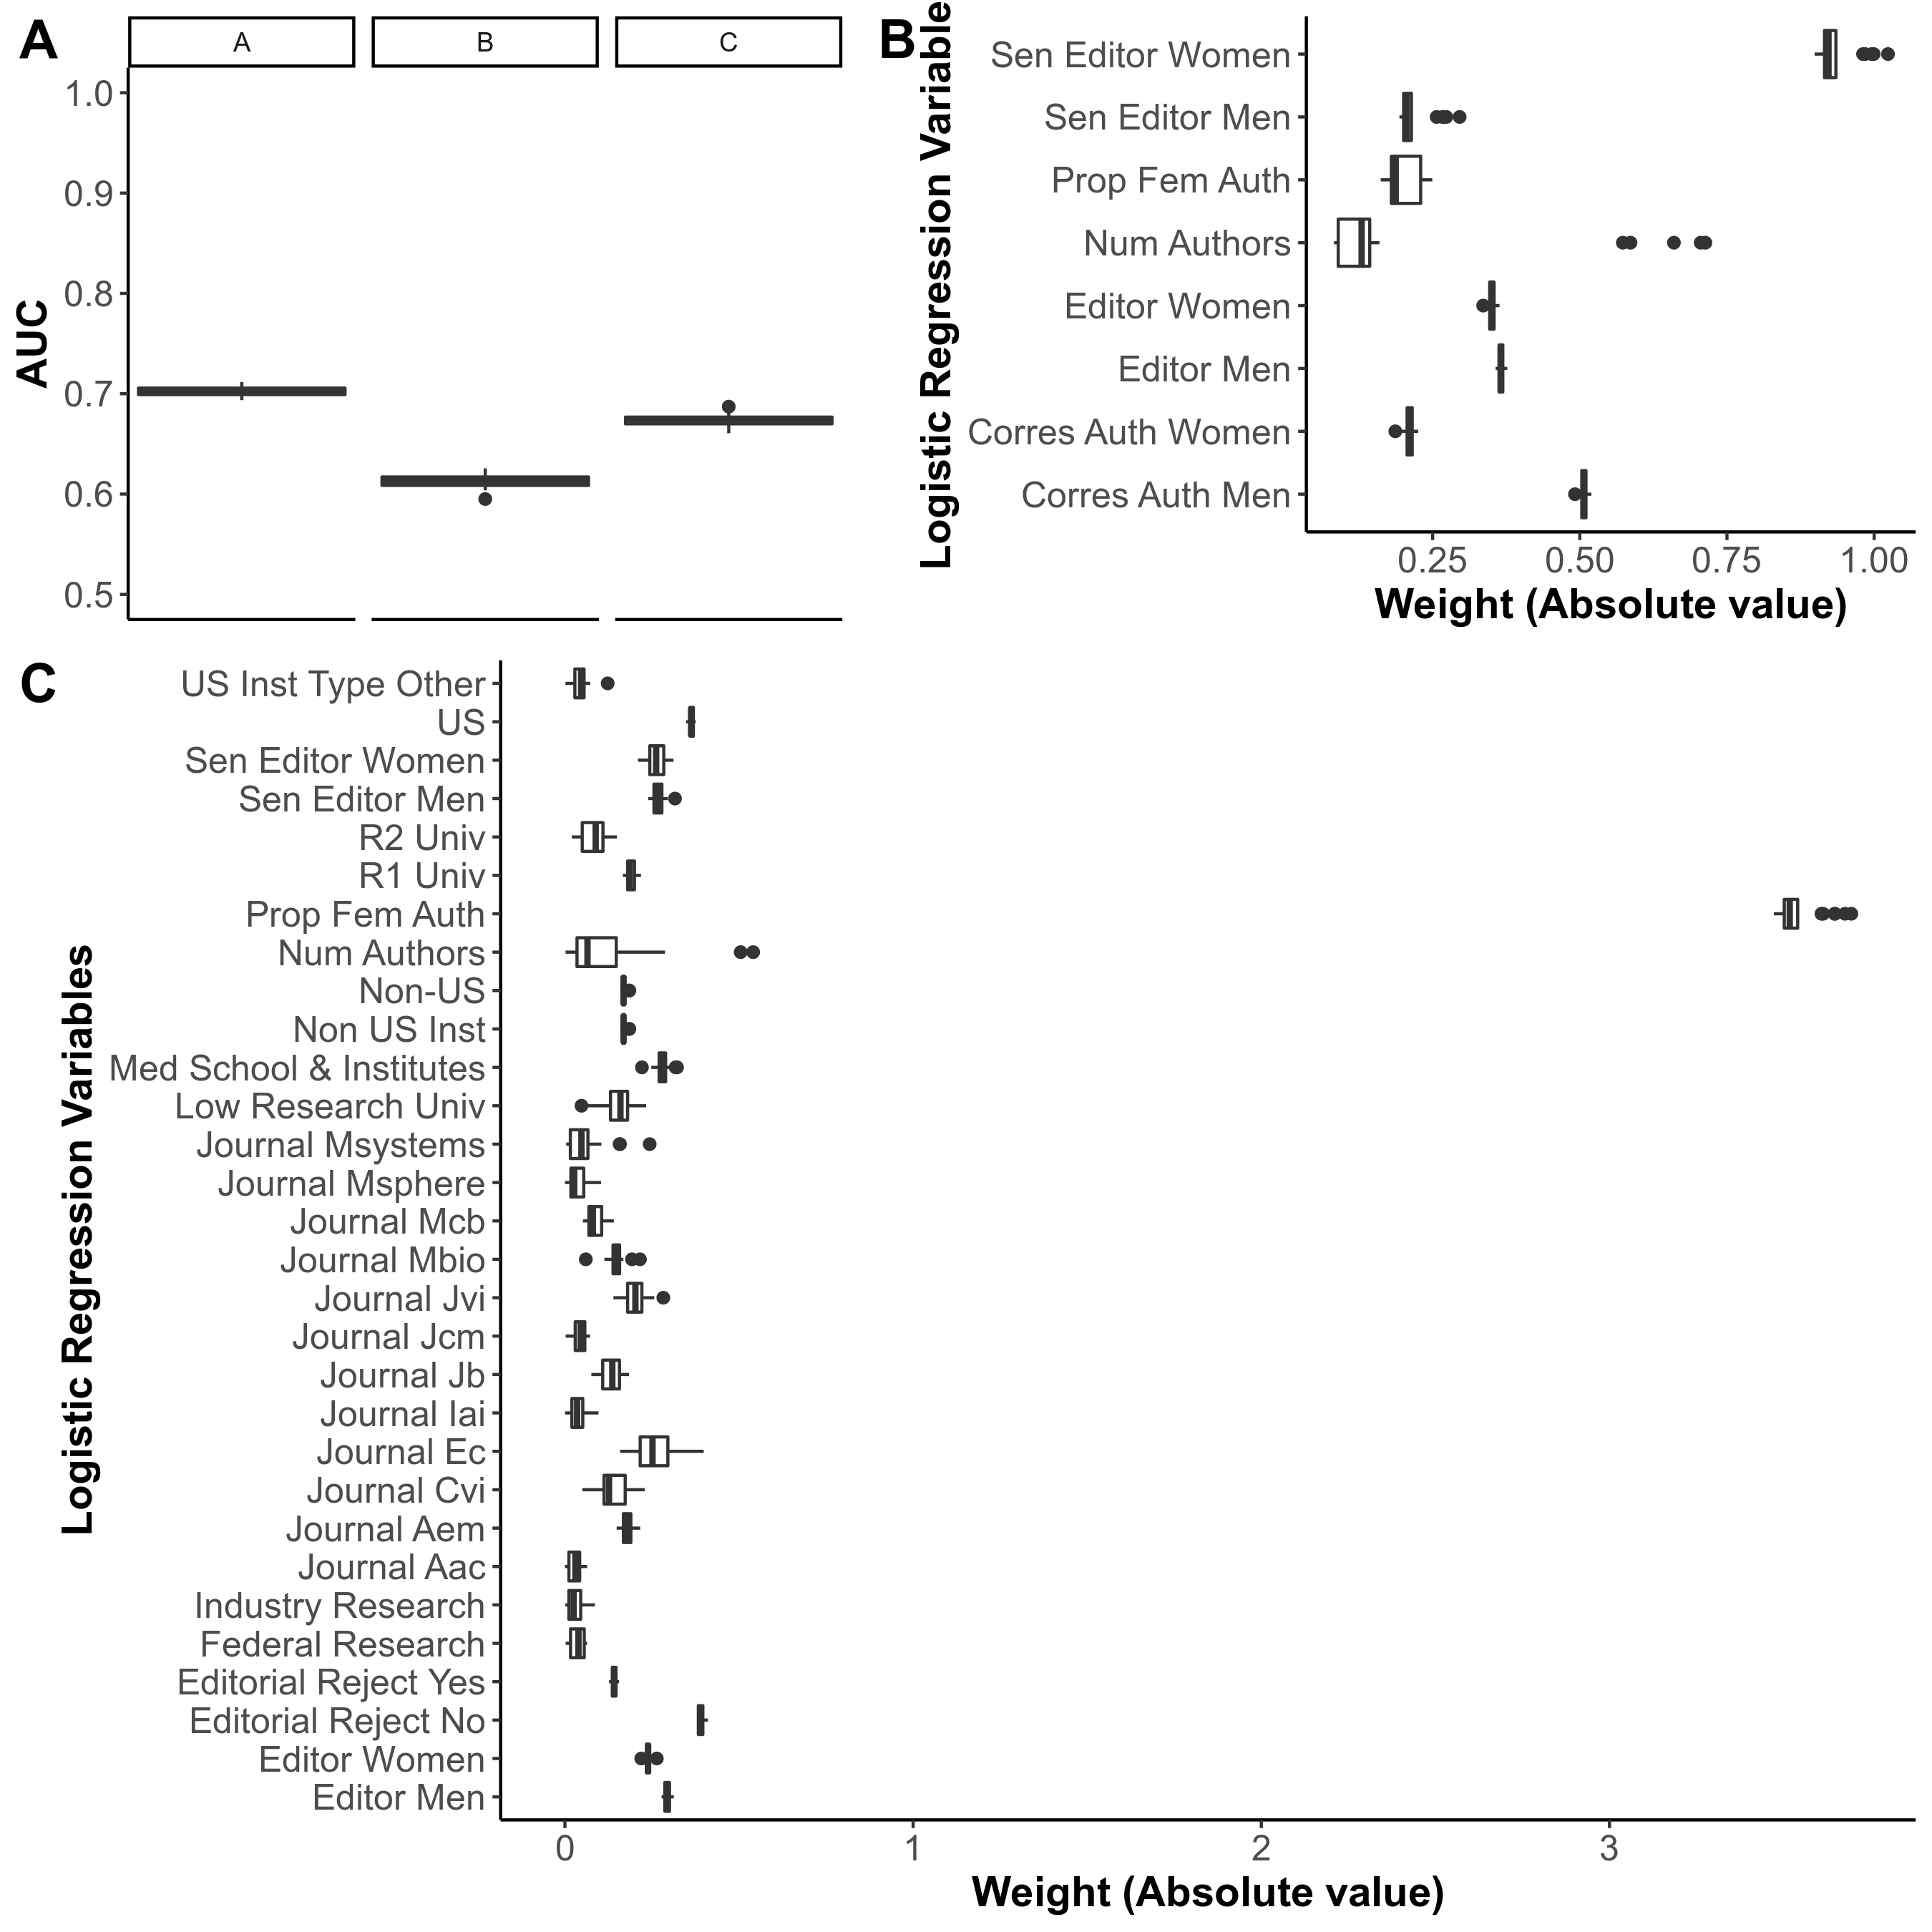
\includegraphics{Figure_S5.png} Figure S5. Comparison of time to final
decision and impact by gender. The number days (A) between when a
manuscript is initially submitted then finally published and (B) that a
manuscript spends in the ASM peer review system. How the impact of
papers published by men (blue) versus women (orange) vary according to
(C) cites and (D) total reads. Citation data includes articles published
between 36 and 48 months prior to August 2018. Total reads includes both
HTML and PDF online views for articles published between 12 and 24
months prior to August 2018. Impact data are divided by the number of
months published.

\newpage

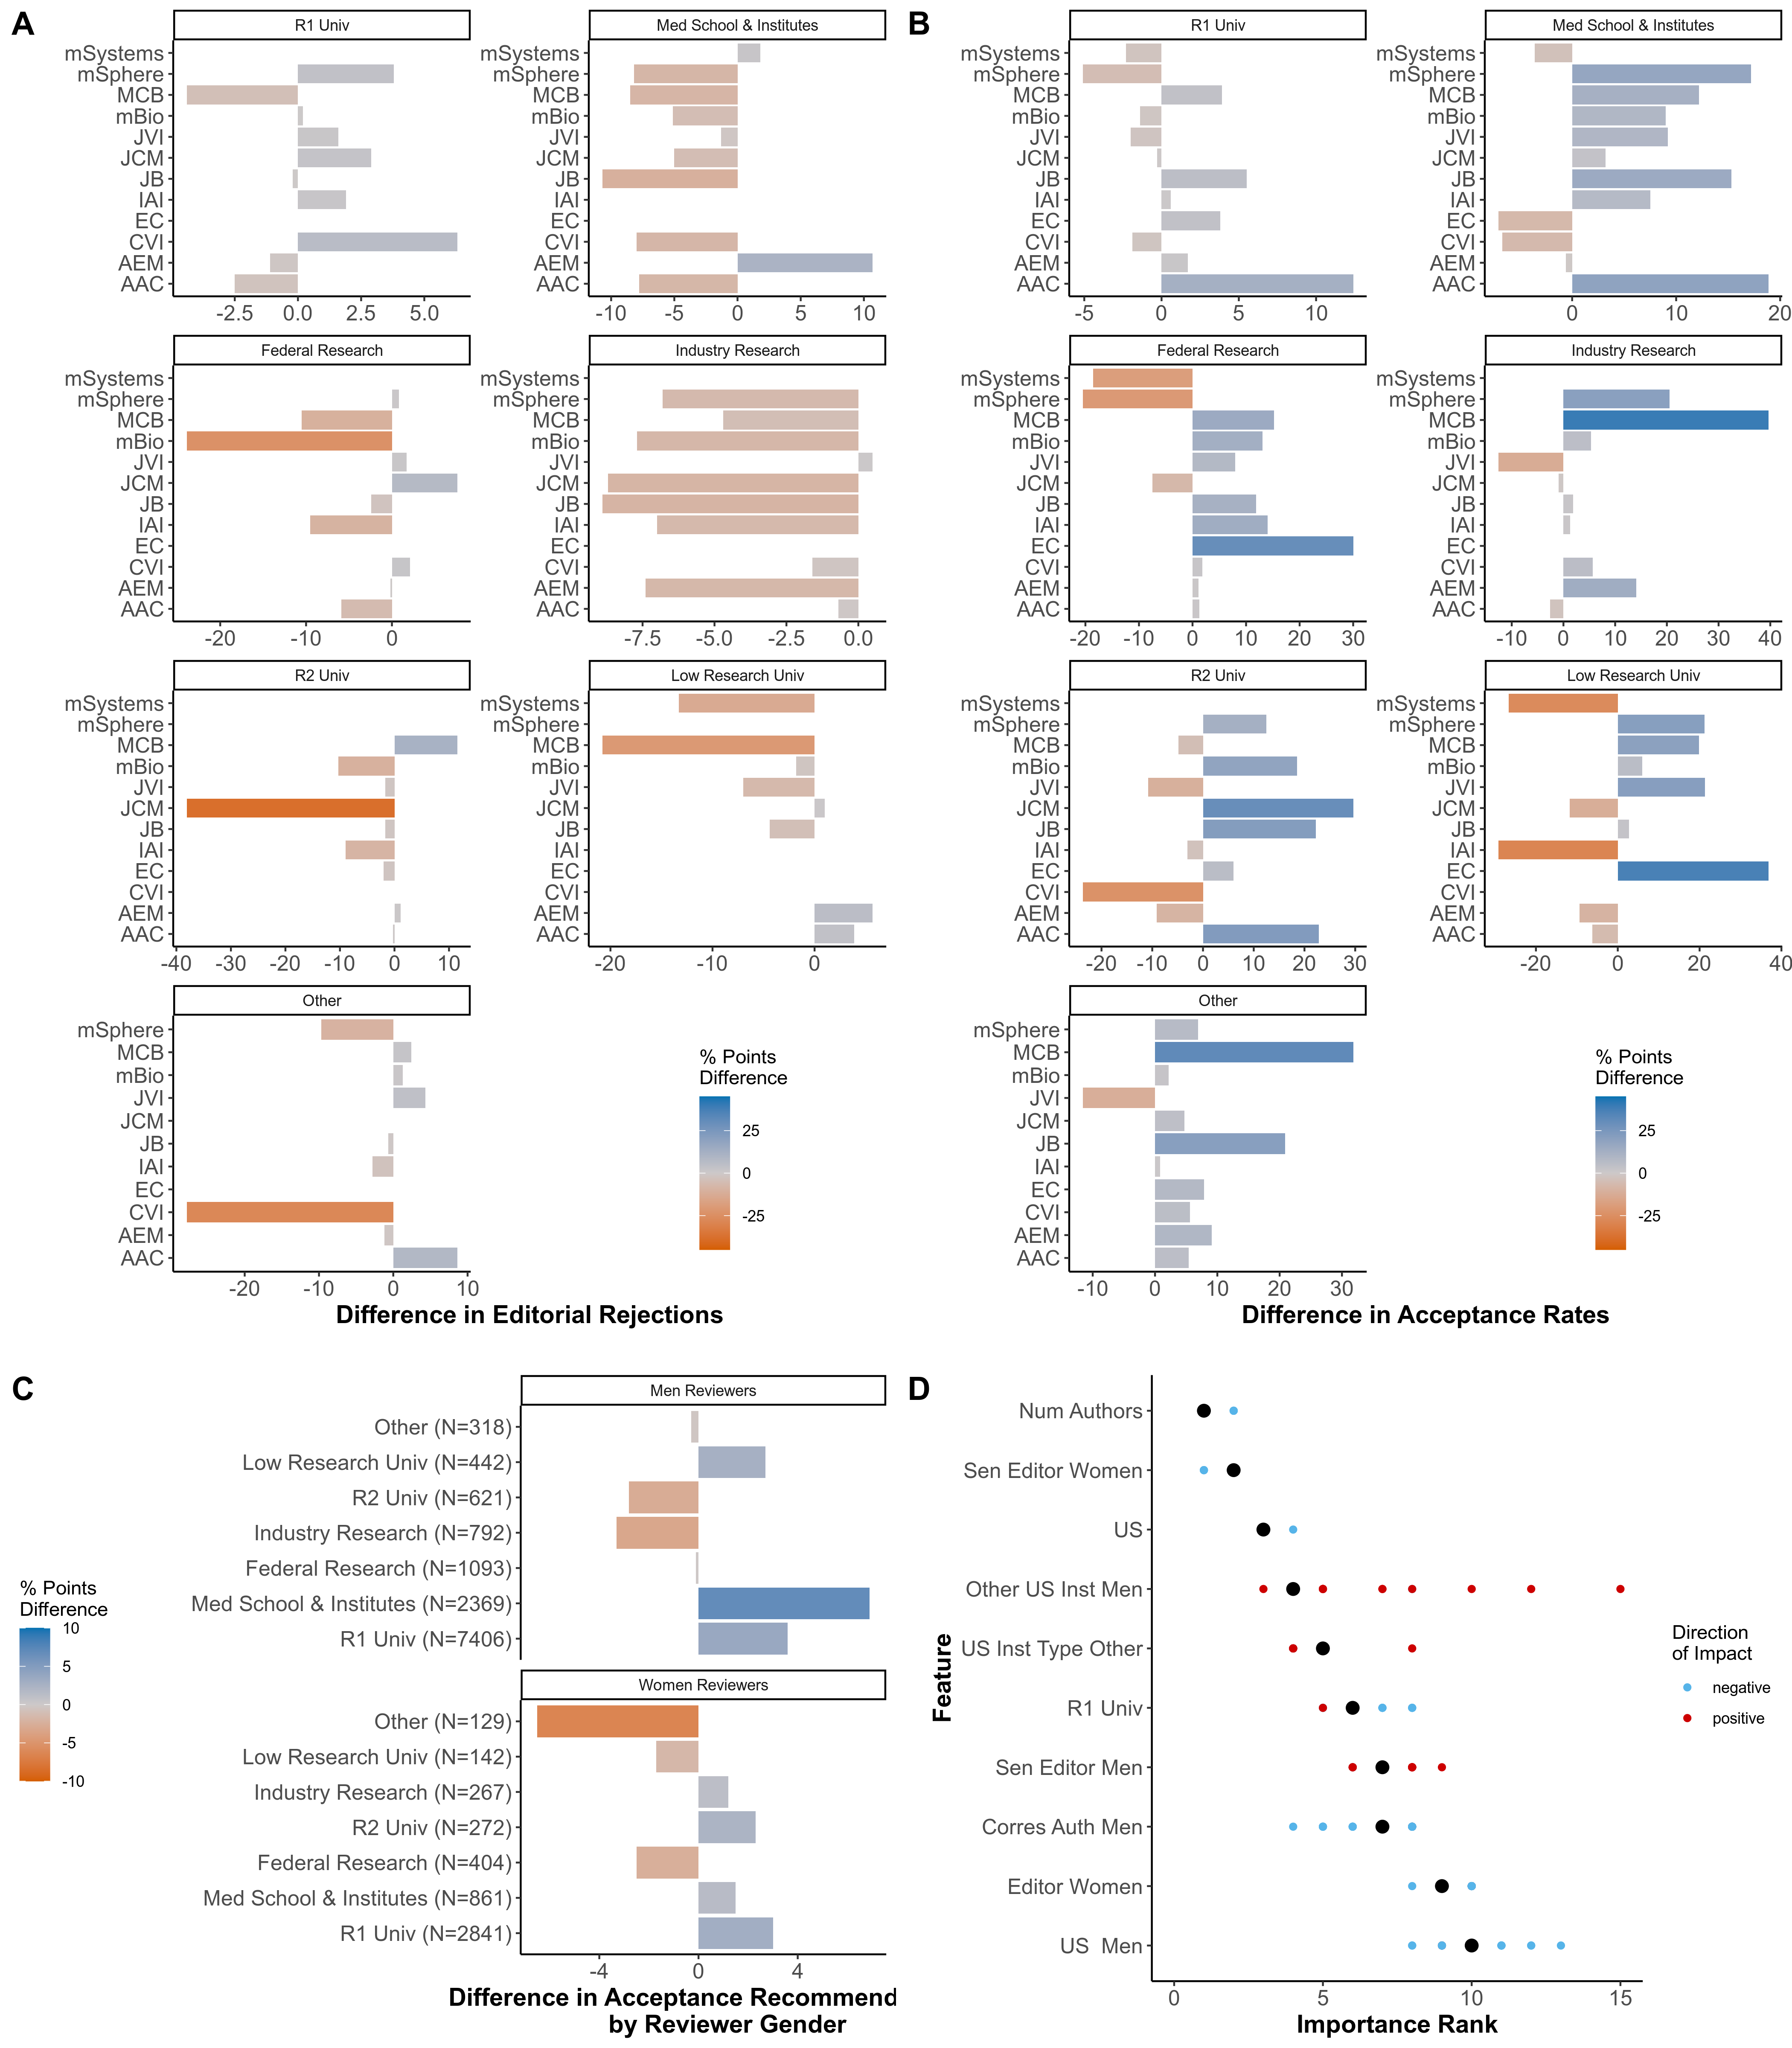
\includegraphics{Figure_S6.png} Figure S6. Difference in acceptance and
rejections by institution type.

\newpage

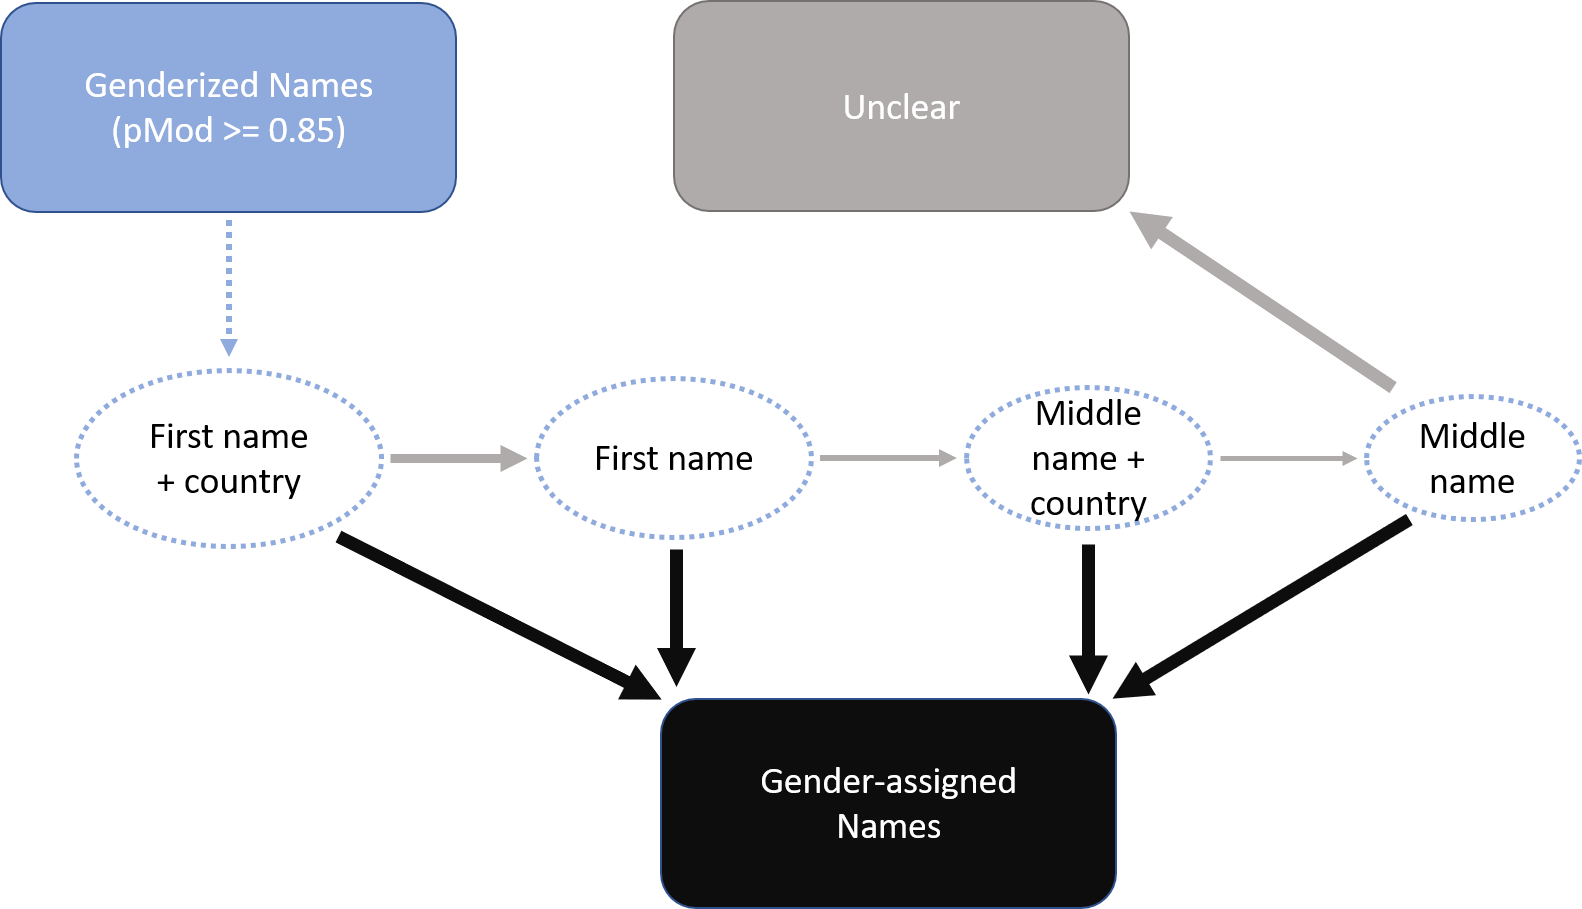
\includegraphics{genderize_method.png} Figure S7. Schematic of gender
prediction and assignment.

\newpage

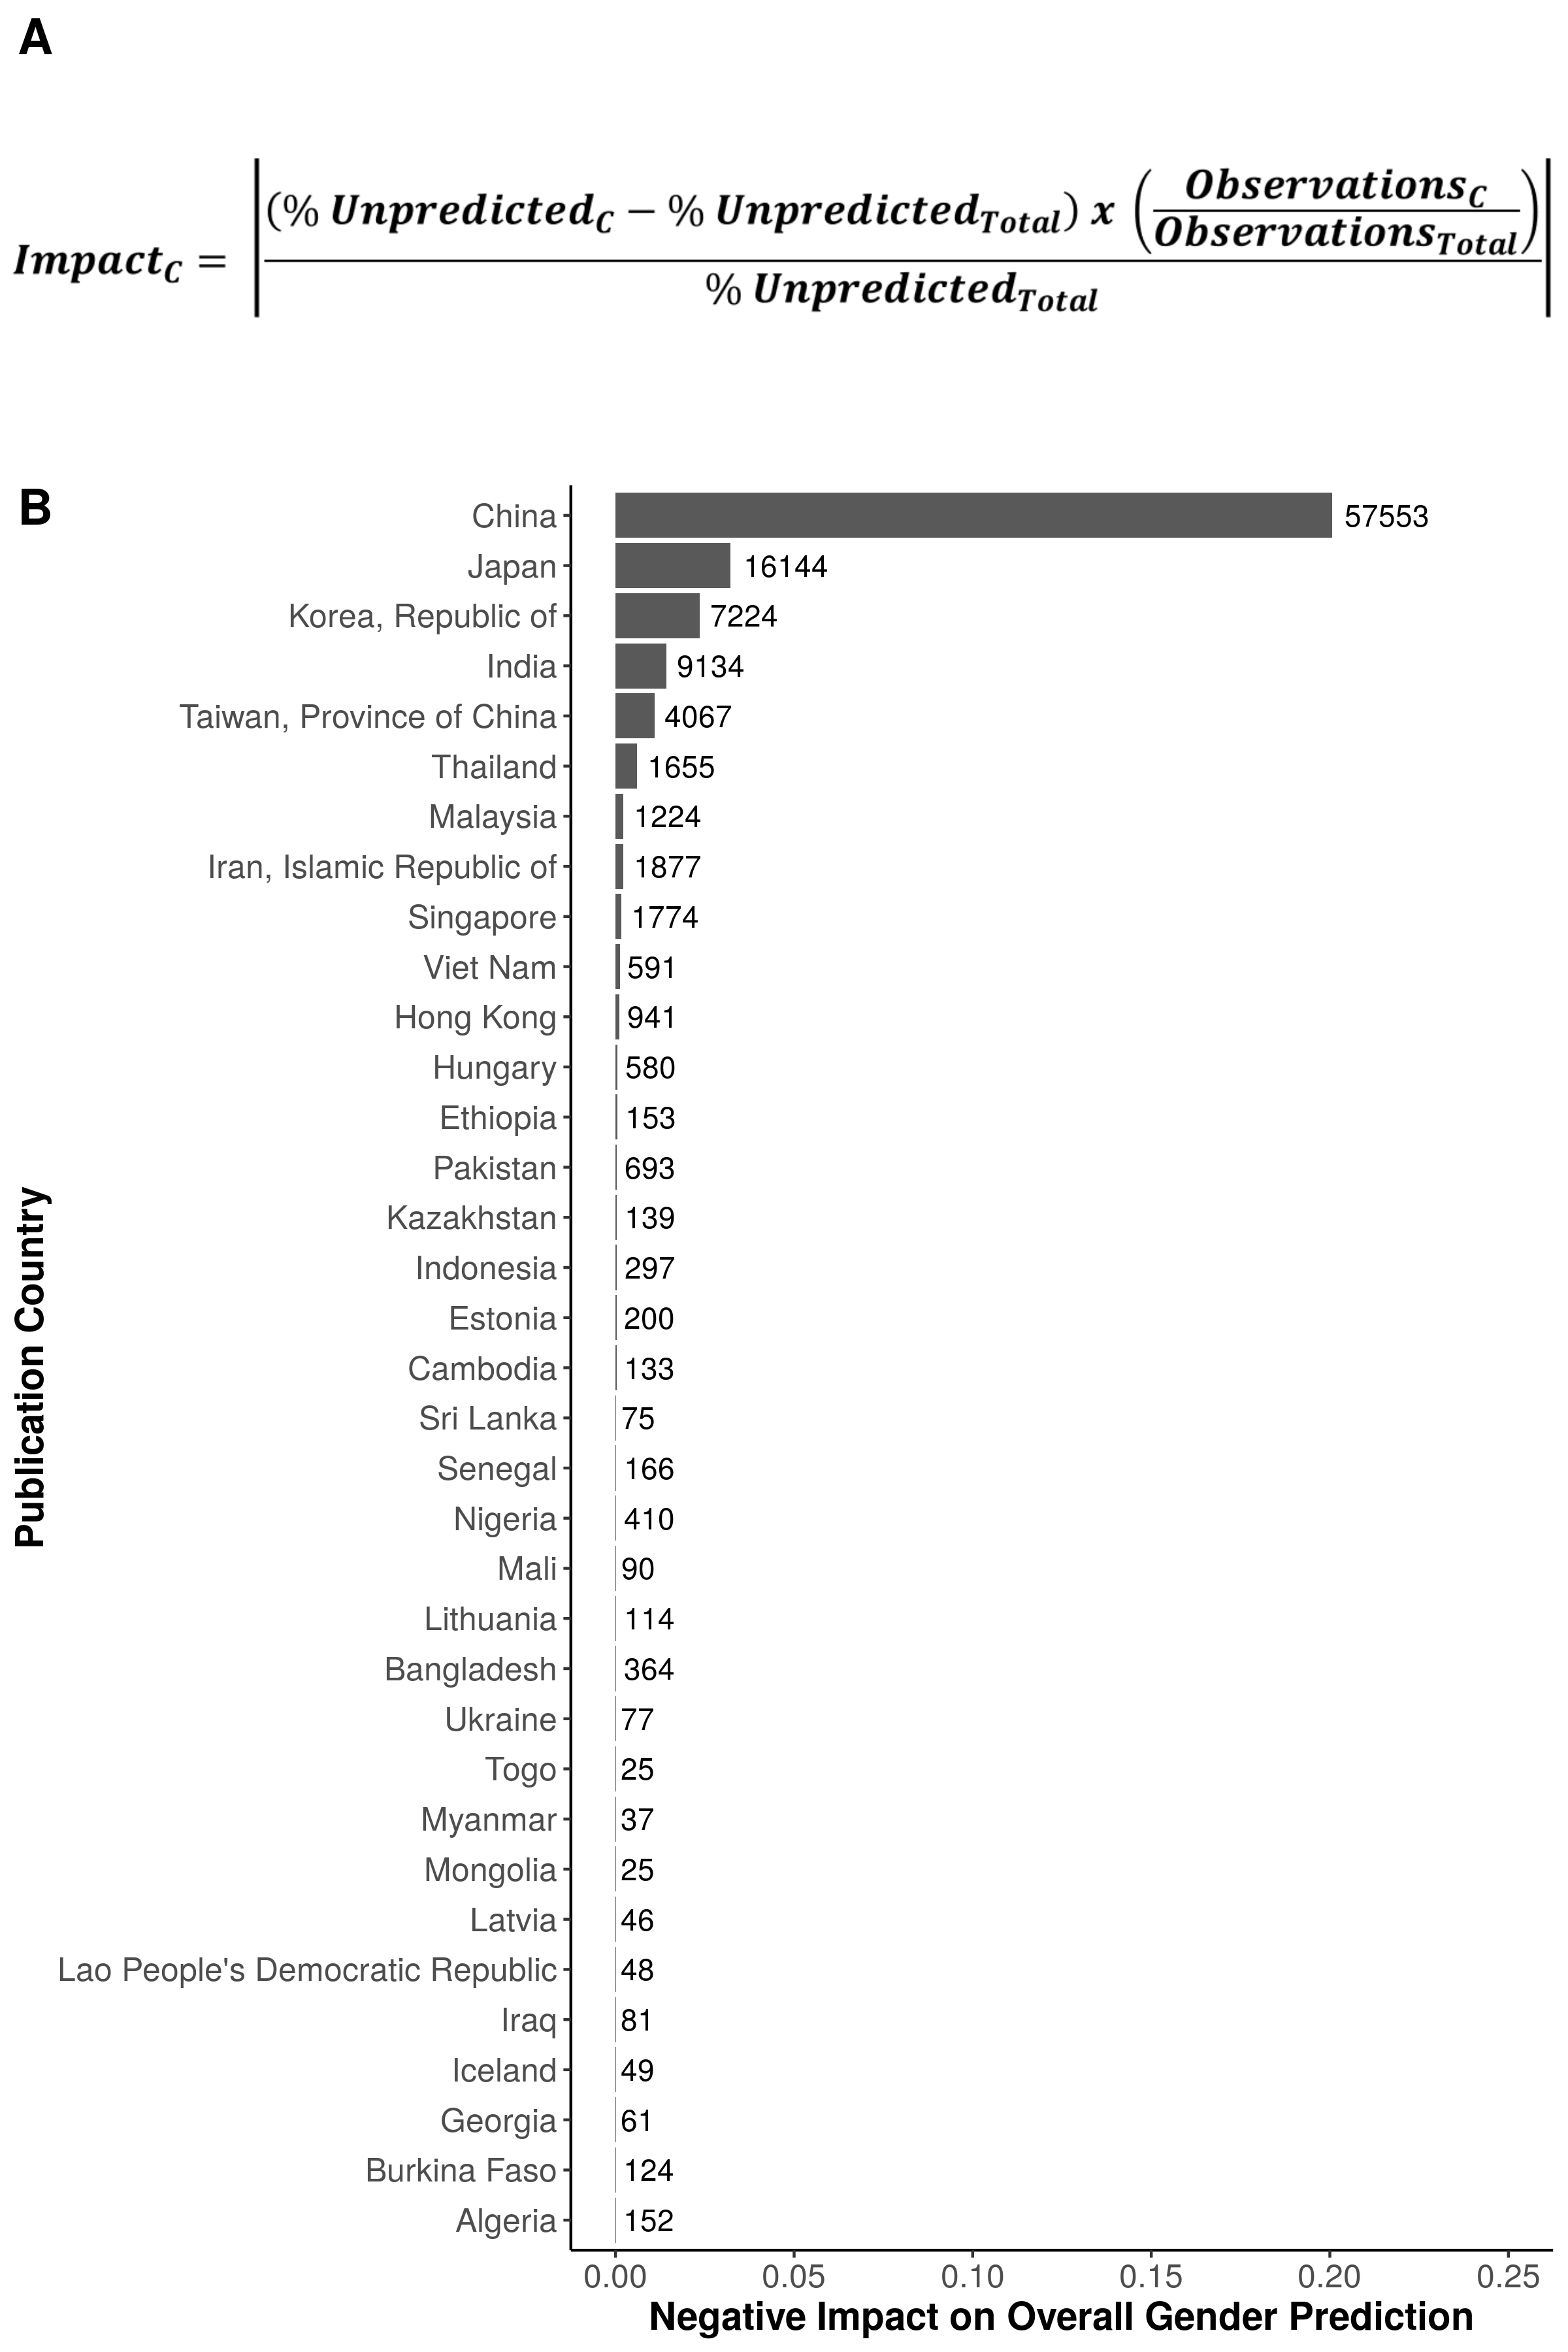
\includegraphics{Figure_S8.png} Figure S8. (A) Equation for calculating
negative bias by genderize. C indicates a country. (B) The negative
impact of each country on the overall gender prediction of the full
data-set. Number is the total n of names associated with each country.

\newpage

\subsection*{References}\label{references}
\addcontentsline{toc}{subsection}{References}

\hypertarget{refs}{}
\hypertarget{ref-sheltzer_elite_2014}{}
1. \textbf{Sheltzer JM}, \textbf{Smith JC}. 2014. Elite male faculty in
the life sciences employ fewer women. Proceedings of the National
Academy of Sciences \textbf{111}:10107--10112.
doi:\href{https://doi.org/10.1073/pnas.1403334111}{10.1073/pnas.1403334111}.

\hypertarget{ref-NCES_condition_2011}{}
2. The condition of education 2012 (NCES 2012-045, Indicator 47) 2012.
U.S. Department of Education, National Center for Education Statistics.

\hypertarget{ref-NCES_full-time_2011}{}
3. Full-time instructional faculty in degree-granting postsecondary
institutions, by race/ethnicity, sex, and academic rank: Fall 2007, fall
2009, and fall 2011. 2013. U.S. Department of Education, National Center
for Education Statistics.

\hypertarget{ref-potvin_diversity_2018}{}
4. \textbf{Potvin DA}, \textbf{Burdfield-Steel E}, \textbf{Potvin JM},
\textbf{Heap SM}. 2018. Diversity begets diversity: A global perspective
on gender equality in scientific society leadership. PLOS ONE
\textbf{13}:e0197280.
doi:\href{https://doi.org/10.1371/journal.pone.0197280}{10.1371/journal.pone.0197280}.

\hypertarget{ref-moss-racusin_science_2012}{}
5. \textbf{Moss-Racusin CA}, \textbf{Dovidio JF}, \textbf{Brescoll VL},
\textbf{Graham MJ}, \textbf{Handelsman J}. 2012. Science faculty's
subtle gender biases favor male students. Proceedings of the National
Academy of Sciences \textbf{109}:16474--16479.
doi:\href{https://doi.org/10.1073/pnas.1211286109}{10.1073/pnas.1211286109}.

\hypertarget{ref-aakhus_gender_2018}{}
6. \textbf{Aakhus E}, \textbf{Mitra N}, \textbf{Lautenbach E},
\textbf{Joffe S}. 2018. Gender and Byline Placement of Co-first Authors
in Clinical and Basic Science Journals With High Impact Factors. JAMA
\textbf{319}:610.
doi:\href{https://doi.org/10.1001/jama.2017.18672}{10.1001/jama.2017.18672}.

\hypertarget{ref-broderick_gender_2019}{}
7. \textbf{Broderick NA}, \textbf{Casadevall A}. 2019. Gender
inequalities among authors who contributed equally. eLife
\textbf{8}:e36399.
doi:\href{https://doi.org/10.7554/eLife.36399}{10.7554/eLife.36399}.

\hypertarget{ref-BlairLoy2017}{}
8. \textbf{Blair-Loy M}, \textbf{Rogers L}, \textbf{Glaser D},
\textbf{Wong Y}, \textbf{Abraham D}, \textbf{Cosman P}. 2017. Gender in
engineering departments: Are there gender differences in interruptions
of academic job talks? Social Sciences \textbf{6}:29.
doi:\href{https://doi.org/10.3390/socsci6010029}{10.3390/socsci6010029}.

\hypertarget{ref-symonds_gender_2006}{}
9. \textbf{Symonds MR}, \textbf{Gemmell NJ}, \textbf{Braisher TL},
\textbf{Gorringe KL}, \textbf{Elgar MA}. 2006. Gender Differences in
Publication Output: Towards an Unbiased Metric of Research Performance.
PLoS ONE \textbf{1}:e127.
doi:\href{https://doi.org/10.1371/journal.pone.0000127}{10.1371/journal.pone.0000127}.

\hypertarget{ref-diprete_cumulative_2006}{}
10. \textbf{DiPrete TA}, \textbf{Eirich GM}. 2006. Cumulative Advantage
as a Mechanism for Inequality: A Review of Theoretical and Empirical
Developments. Annual Review of Sociology \textbf{32}:271--297.
doi:\href{https://doi.org/10.1146/annurev.soc.32.061604.123127}{10.1146/annurev.soc.32.061604.123127}.

\hypertarget{ref-thebaud_segregation_2018}{}
11. \textbf{Thébaud S}, \textbf{Charles M}. 2018. Segregation,
Stereotypes, and STEM. Social Sciences \textbf{7}:111.
doi:\href{https://doi.org/10.3390/socsci7070111}{10.3390/socsci7070111}.

\hypertarget{ref-lerback_journals_2017}{}
12. \textbf{Lerback J}, \textbf{Hanson B}. 2017. Journals invite too few
women to referee. Nature \textbf{541}:455--457.
doi:\href{https://doi.org/10.1038/541455a}{10.1038/541455a}.

\hypertarget{ref-fox_editor_2016}{}
13. \textbf{Fox CW}, \textbf{Burns CS}, \textbf{Meyer JA}. 2016. Editor
and reviewer gender influence the peer review process but not peer
review outcomes at an ecology journal. Functional Ecology
\textbf{30}:140--153.
doi:\href{https://doi.org/10.1111/1365-2435.12529}{10.1111/1365-2435.12529}.

\hypertarget{ref-ceci_understanding_2011}{}
14. \textbf{Ceci SJ}, \textbf{Williams WM}. 2011. Understanding current
causes of women's underrepresentation in science. Proceedings of the
National Academy of Sciences \textbf{108}:3157--3162.
doi:\href{https://doi.org/10.1073/pnas.1014871108}{10.1073/pnas.1014871108}.

\hypertarget{ref-handley_examination_2015}{}
15. \textbf{Handley G}, \textbf{Frantz CM}, \textbf{Kocovsky PM},
\textbf{DeVries DR}, \textbf{Cooke SJ}, \textbf{Claussen J}. 2015. An
Examination of Gender Differences in the American Fisheries Society
Peer-Review Process. Fisheries \textbf{40}:442--451.
doi:\href{https://doi.org/10.1080/03632415.2015.1059824}{10.1080/03632415.2015.1059824}.

\hypertarget{ref-edwards_gender_2018}{}
16. \textbf{Edwards HA}, \textbf{Schroeder J}, \textbf{Dugdale HL}.
2018. Gender differences in authorships are not associated with
publication bias in an evolutionary journal. PLOS ONE
\textbf{13}:e0201725.
doi:\href{https://doi.org/10.1371/journal.pone.0201725}{10.1371/journal.pone.0201725}.

\hypertarget{ref-buckley_is_2014}{}
17. \textbf{Buckley HL}, \textbf{Sciligo AR}, \textbf{Adair KL},
\textbf{Case BS}, \textbf{Monks JM}. 2014. Is there gender bias in
reviewer selection and publication success rates for the. New Zealand
Journal of Ecology \textbf{38}:5.

\hypertarget{ref-Murray400515}{}
18. \textbf{Murray D}, \textbf{Siler K}, \textbf{Larivière V},
\textbf{Chan WM}, \textbf{Collings AM}, \textbf{Raymond J},
\textbf{Sugimoto CR}. 2019. Author-reviewer homophily in peer review.
bioRxiv. doi:\href{https://doi.org/10.1101/400515}{10.1101/400515}.

\hypertarget{ref-fox_gender_2019}{}
19. \textbf{Fox CW}, \textbf{Paine CET}. 2019. Gender differences in
peer review outcomes and manuscript impact at six journals of ecology
and evolution. Ecology and Evolution \textbf{9}:3599--3619.
doi:\href{https://doi.org/10.1002/ece3.4993}{10.1002/ece3.4993}.

\hypertarget{ref-allagnat_gender_2017}{}
20. \textbf{Allagnat L}, \textbf{Berghmans S}, \textbf{Falk-Krzesinski
HJ}, \textbf{Hanafi S}, \textbf{Herbert R}, \textbf{Huggett S},
\textbf{Tobin S}. 2017. Gender in the global research landscape.

\hypertarget{ref-erin_hengel_publishing_2017}{}
21. \textbf{Erin Hengel}. 2017. Publishing while female 1--64.
doi:\href{https://doi.org/10.17863/CAM.17548}{10.17863/CAM.17548}.

\hypertarget{ref-weeden_degrees_2017}{}
22. \textbf{Weeden K}, \textbf{Thébaud S}, \textbf{Gelbgiser D}. 2017.
Degrees of Difference: Gender Segregation of U.S. Doctorates by Field
and Program Prestige. Sociological Science \textbf{4}:123--150.
doi:\href{https://doi.org/10.15195/v4.a6}{10.15195/v4.a6}.

\hypertarget{ref-Martinez2007}{}
23. \textbf{Martinez ED}, \textbf{Botos J}, \textbf{Dohoney KM},
\textbf{Geiman TM}, \textbf{Kolla SS}, \textbf{Olivera A}, \textbf{Qiu
Y}, \textbf{Rayasam GV}, \textbf{Stavreva DA}, \textbf{Cohen-Fix O}.
2007. Falling off the academic bandwagon. women are more likely to quit
at the postdoc to principal investigator transition. EMBO reports
\textbf{8}:977--981.
doi:\href{https://doi.org/10.1038/sj.embor.7401110}{10.1038/sj.embor.7401110}.

\hypertarget{ref-debarre_gender_2018}{}
24. \textbf{Débarre F}, \textbf{Rode NO}, \textbf{Ugelvig LV}. 2018.
Gender equity at scientific events. Evolution Letters
\textbf{2}:148--158.
doi:\href{https://doi.org/10.1002/evl3.49}{10.1002/evl3.49}.

\hypertarget{ref-sardelis_not_2016}{}
25. \textbf{Sardelis S}, \textbf{Drew JA}. 2016. Not ``Pulling up the
Ladder'': Women Who Organize Conference Symposia Provide Greater
Opportunities for Women to Speak at Conservation Conferences. PLOS ONE
\textbf{11}:e0160015.
doi:\href{https://doi.org/10.1371/journal.pone.0160015}{10.1371/journal.pone.0160015}.

\hypertarget{ref-casadevall_presence_2014}{}
26. \textbf{Casadevall A}, \textbf{Handelsman J}. 2014. The Presence of
Female Conveners Correlates with a Higher Proportion of Female Speakers
at Scientific Symposia. mBio \textbf{5}:e00846--13--e00846--13.
doi:\href{https://doi.org/10.1128/mBio.00846-13}{10.1128/mBio.00846-13}.

\hypertarget{ref-guarino_faculty_2017}{}
27. \textbf{Guarino CM}, \textbf{Borden VMH}. 2017. Faculty Service
Loads and Gender: Are Women Taking Care of the Academic Family? Research
in Higher Education \textbf{58}:672--694.
doi:\href{https://doi.org/10.1007/s11162-017-9454-2}{10.1007/s11162-017-9454-2}.

\hypertarget{ref-Dotson2012}{}
28. \textbf{Dotson K}. 2012. HOW IS THIS PAPER PHILOSOPHY? Comparative
Philosophy: An International Journal of Constructive Engagement of
Distinct Approaches toward World Philosophy \textbf{3}.
doi:\href{https://doi.org/10.31979/2151-6014(2012).030105}{10.31979/2151-6014(2012).030105}.

\hypertarget{ref-Dotson2014}{}
29. \textbf{Dotson K}. 2014. Conceptualizing epistemic oppression.
Social Epistemology \textbf{28}:115--138.
doi:\href{https://doi.org/10.1080/02691728.2013.782585}{10.1080/02691728.2013.782585}.

\hypertarget{ref-settles_epistemic_2019}{}
30. \textbf{Settles I}, \textbf{Jones M}, \textbf{Buchanan N},
\textbf{Dotson K}. 2019. Epistemic exclusion: Gatekeeping that
marginalizes faculty of color. Working Paper.

\hypertarget{ref-macaluso_is_2016}{}
31. \textbf{Macaluso B}, \textbf{Larivière V}, \textbf{Sugimoto T},
\textbf{Sugimoto CR}. 2016. Is Science Built on the Shoulders of Women?
A Study of Gender Differences in Contributorship: Academic Medicine
\textbf{91}:1136--1142.
doi:\href{https://doi.org/10.1097/ACM.0000000000001261}{10.1097/ACM.0000000000001261}.

\hypertarget{ref-gilbert_is_1994}{}
32. \textbf{Gilbert JR}, \textbf{Williams ES}. 1994. Is There Gender
Bias in JAMA's Peer Review Process? 4.

\hypertarget{ref-holman_researchers_2019}{}
33. \textbf{Holman L}, \textbf{Morandin C}. 2019. Researchers
collaborate with same-gendered colleagues more often than expected
across the life sciences. PLOS ONE \textbf{14}:e0216128.
doi:\href{https://doi.org/10.1371/journal.pone.0216128}{10.1371/journal.pone.0216128}.

\hypertarget{ref-fox_citations_2016}{}
34. \textbf{Fox CW}, \textbf{Paine CET}, \textbf{Sauterey B}. 2016.
Citations increase with manuscript length, author number, and references
cited in ecology journals. Ecology and Evolution \textbf{6}:7717--7726.
doi:\href{https://doi.org/10.1002/ece3.2505}{10.1002/ece3.2505}.

\hypertarget{ref-wiedman_rewarding_2019}{}
35. \textbf{Wiedman C}. 2019. Rewarding Collaborative Research: Role
Congruity Bias and the Gender Pay Gap in Academe. Journal of Business
Ethics.
doi:\href{https://doi.org/10.1007/s10551-019-04165-0}{10.1007/s10551-019-04165-0}.

\hypertarget{ref-berg_examining_2019}{}
36. \textbf{Berg J}. 2019. Examining author gender data. Science
\textbf{363}:7--7.
doi:\href{https://doi.org/10.1126/science.aaw4633}{10.1126/science.aaw4633}.

\hypertarget{ref-conley_call_2012-1}{}
37. \textbf{Conley D}, \textbf{Stadmark J}. 2012. A call to commission
more women writers. Nature \textbf{488}:590--590.
doi:\href{https://doi.org/10.1038/488590a}{10.1038/488590a}.

\hypertarget{ref-bendels_gender_2018}{}
38. \textbf{Bendels MHK}, \textbf{Müller R}, \textbf{Brueggmann D},
\textbf{Groneberg DA}. 2018. Gender disparities in high-quality research
revealed by Nature Index journals. PLOS ONE \textbf{13}:e0189136.
doi:\href{https://doi.org/10.1371/journal.pone.0189136}{10.1371/journal.pone.0189136}.

\hypertarget{ref-Shen275362}{}
39. \textbf{Shen YA}, \textbf{Webster JM}, \textbf{Shoda Y},
\textbf{Fine I}. 2018. Persistent underrepresentation of womens science
in high profile journals. bioRxiv.
doi:\href{https://doi.org/10.1101/275362}{10.1101/275362}.

\hypertarget{ref-Kaatz2014}{}
40. \textbf{Kaatz A}, \textbf{Gutierrez B}, \textbf{Carnes M}. 2014.
Threats to objectivity in peer review: The case of gender. Trends in
Pharmacological Sciences \textbf{35}:371--373.
doi:\href{https://doi.org/10.1016/j.tips.2014.06.005}{10.1016/j.tips.2014.06.005}.

\hypertarget{ref-Carnes2005}{}
41. \textbf{Carnes M}, \textbf{Geller S}, \textbf{Fine E},
\textbf{Sheridan J}, \textbf{Handelsman J}. 2005. NIH directors pioneer
awards: Could the selection process be biased against women? Journal of
Womens Health \textbf{14}:684--691.
doi:\href{https://doi.org/10.1089/jwh.2005.14.684}{10.1089/jwh.2005.14.684}.

\hypertarget{ref-babcock_women_2003}{}
42. \textbf{Babcock L}, \textbf{Laschever S}. 2003. Women don't ask:
Negotiation and the gender divide. Princeton University Press,
Princeton, N.J.

\hypertarget{ref-MILLER1992}{}
43. \textbf{MILLER LC}, \textbf{COOKE L}, \textbf{TSANG J},
\textbf{MORGAN F}. 1992. Should i brag? Nature and impact of positive
and boastful disclosures for women and men. Human Communication Research
\textbf{18}:364--399.
doi:\href{https://doi.org/10.1111/j.1468-2958.1992.tb00557.x}{10.1111/j.1468-2958.1992.tb00557.x}.

\hypertarget{ref-Kolev2019}{}
44. \textbf{Kolev J}, \textbf{Fuentes-Medel Y}, \textbf{Murray F}. 2019.
Is blinded review enough? How gendered outcomes arise even under
anonymous evaluation. National Bureau of Economic Research.

\hypertarget{ref-Hagan_2019}{}
45. \textbf{Hagan \textnormal{Ada K.}}, \textbf{Pollet RM},
\textbf{Libertucci J}. 2019. Policy should change to improve invited
speaker diversity and reflect trainee diversity. bioRxiv.

\hypertarget{ref-fox_gender_2016}{}
46. \textbf{Fox CW}, \textbf{Burns CS}, \textbf{Muncy AD}, \textbf{Meyer
JA}. 2016. Gender differences in patterns of authorship do not affect
peer review outcomes at an ecology journal. Functional Ecology
\textbf{30}:126--139.
doi:\href{https://doi.org/10.1111/1365-2435.12587}{10.1111/1365-2435.12587}.

\hypertarget{ref-cox_case_2018}{}
47. \textbf{Cox AR}, \textbf{Montgomerie R}. 2018. The Case For and
Against Double-blind Reviews. preprint, Scientific Communication;
Education.

\hypertarget{ref-applebaum_remediating_2019}{}
48. \textbf{Applebaum B}. 2019. Remediating Campus Climate: Implicit
Bias Training is Not Enough. Studies in Philosophy and Education
\textbf{38}:129--141.
doi:\href{https://doi.org/10.1007/s11217-018-9644-1}{10.1007/s11217-018-9644-1}.

\hypertarget{ref-Holmes2011}{}
49. \textbf{Holmes MA}, \textbf{Asher P}, \textbf{Farrington J},
\textbf{Fine R}, \textbf{Leinen MS}, \textbf{LeBoy P}. 2011. Does gender
bias influence awards given by societies? Eos, Transactions American
Geophysical Union \textbf{92}:421--422.
doi:\href{https://doi.org/10.1029/2011eo470002}{10.1029/2011eo470002}.

\hypertarget{ref-Malouff2016}{}
50. \textbf{Malouff JM}, \textbf{Thorsteinsson EB}. 2016. Bias in
grading: A meta-analysis of experimental research findings. Australian
Journal of Education \textbf{60}:245--256.
doi:\href{https://doi.org/10.1177/0004944116664618}{10.1177/0004944116664618}.

\hypertarget{ref-Reddy2010}{}
51. \textbf{Reddy YM}, \textbf{Andrade H}. 2010. A review of rubric use
in higher education. Assessment \& Evaluation in Higher Education
\textbf{35}:435--448.
doi:\href{https://doi.org/10.1080/02602930902862859}{10.1080/02602930902862859}.

\hypertarget{ref-Rezaei2010}{}
52. \textbf{Rezaei AR}, \textbf{Lovorn M}. 2010. Reliability and
validity of rubrics for assessment through writing. Assessing Writing
\textbf{15}:18--39.
doi:\href{https://doi.org/10.1016/j.asw.2010.01.003}{10.1016/j.asw.2010.01.003}.

\hypertarget{ref-R_software_2017}{}
53. \textbf{R Core Team}. 2017. R: A language and environment for
statistical computing. R Foundation for Statistical Computing, Vienna,
Austria.

\hypertarget{ref-wickham_tidyverse_2017}{}
54. \textbf{Wickham H}. 2017. Tidyverse: Easily Install and Load the
'Tidyverse'.

\hypertarget{ref-duncan_xml_2018}{}
55. \textbf{CRAN Team DTL and the}. 2018. XML: Tools for Parsing and
Generating XML Within R and S-Plus.

\hypertarget{ref-wickham_xml2_2018}{}
56. \textbf{Wickham H}, \textbf{Hester J}, \textbf{Ooms J}. 2018. Xml2:
Parse XML.

\hypertarget{ref-grolemund_dates_2011}{}
57. \textbf{Grolemund G}, \textbf{Wickham H}. 2011. Dates and Times Made
Easy with lubridate. Journal of Statistical Software \textbf{40}:1--25.

\hypertarget{ref-wickham_scales_2018}{}
58. \textbf{Wickham H}. 2018. Scales: Scale Functions for Visualization.

\hypertarget{ref-neuwirth_rcolorbrewer_2014}{}
59. \textbf{Neuwirth E}. 2014. RColorBrewer: ColorBrewer Palettes.

\hypertarget{ref-cowplot}{}
60. \textbf{Wilke CO}. 2019. Cowplot: Streamlined plot theme and plot
annotations for 'ggplot2'.

\hypertarget{ref-rlang}{}
61. \textbf{Henry L}, \textbf{Wickham H}. 2019. Rlang: Functions for
base types and core r and 'tidyverse' features.

\hypertarget{ref-formattable}{}
62. \textbf{Ren K}, \textbf{Russell K}. 2016. Formattable: Create
'formattable' data structures.

\hypertarget{ref-knitr_2018}{}
63. \textbf{Xie Y}. 2018. Knitr: A general-purpose package for dynamic
report generation in r.

\hypertarget{ref-knitr_2014}{}
64. \textbf{Xie Y}. 2014. Knitr: A comprehensive tool for reproducible
research in R. \emph{In} Stodden, V, Leisch, F, Peng, RD (eds.),
Implementing reproducible computational research. Chapman; Hall/CRC.

\hypertarget{ref-rmd_rstudio}{}
65. \textbf{Allaire J}, \textbf{Xie Y}, \textbf{McPherson J},
\textbf{Luraschi J}, \textbf{Ushey K}, \textbf{Atkins A},
\textbf{Wickham H}, \textbf{Cheng J}, \textbf{Chang W}, \textbf{Iannone
R}. 2018. Rmarkdown: Dynamic documents for r.

\hypertarget{ref-rmd_book}{}
66. \textbf{Xie Y}, \textbf{Allaire J}, \textbf{Grolemund G}. 2018. R
markdown: The definitive guide. Chapman; Hall/CRC, Boca Raton, Florida.

\hypertarget{ref-markdown}{}
67. \textbf{Allaire J}, \textbf{Horner J}, \textbf{Xie Y}, \textbf{Marti
V}, \textbf{Porte N}. 2018. Markdown: 'Markdown' rendering for r.

\hypertarget{ref-Carnegie2018}{}
68. \textbf{Postsecondary Research IUC for}. 2018. Carnegie
classification of institutions of higher education.

\hypertarget{ref-caddigan_genderguesser}{}
69. \textbf{Caddigan E}. GenderGuesser: Guess the gender of a name.

\hypertarget{ref-khun_caret_2018}{}
70. \textbf{Khun M}. 2018. Caret: Classification and Regression
Training. R package version 6.0-81.


\end{document}
